\documentclass[twoside]{book}

% Packages required by doxygen
\usepackage{fixltx2e}
\usepackage{calc}
\usepackage{doxygen}
\usepackage[export]{adjustbox} % also loads graphicx
\usepackage{graphicx}
\usepackage[utf8]{inputenc}
\usepackage{makeidx}
\usepackage{multicol}
\usepackage{multirow}
\PassOptionsToPackage{warn}{textcomp}
\usepackage{textcomp}
\usepackage[nointegrals]{wasysym}
\usepackage[table]{xcolor}

% Font selection
\usepackage[T1]{fontenc}
\usepackage[scaled=.90]{helvet}
\usepackage{courier}
\usepackage{amssymb}
\usepackage{sectsty}
\renewcommand{\familydefault}{\sfdefault}
\allsectionsfont{%
  \fontseries{bc}\selectfont%
  \color{darkgray}%
}
\renewcommand{\DoxyLabelFont}{%
  \fontseries{bc}\selectfont%
  \color{darkgray}%
}
\newcommand{\+}{\discretionary{\mbox{\scriptsize$\hookleftarrow$}}{}{}}

% Page & text layout
\usepackage{geometry}
\geometry{%
  a4paper,%
  top=2.5cm,%
  bottom=2.5cm,%
  left=2.5cm,%
  right=2.5cm%
}
\tolerance=750
\hfuzz=15pt
\hbadness=750
\setlength{\emergencystretch}{15pt}
\setlength{\parindent}{0cm}
\setlength{\parskip}{3ex plus 2ex minus 2ex}
\makeatletter
\renewcommand{\paragraph}{%
  \@startsection{paragraph}{4}{0ex}{-1.0ex}{1.0ex}{%
    \normalfont\normalsize\bfseries\SS@parafont%
  }%
}
\renewcommand{\subparagraph}{%
  \@startsection{subparagraph}{5}{0ex}{-1.0ex}{1.0ex}{%
    \normalfont\normalsize\bfseries\SS@subparafont%
  }%
}
\makeatother

% Headers & footers
\usepackage{fancyhdr}
\pagestyle{fancyplain}
\fancyhead[LE]{\fancyplain{}{\bfseries\thepage}}
\fancyhead[CE]{\fancyplain{}{}}
\fancyhead[RE]{\fancyplain{}{\bfseries\leftmark}}
\fancyhead[LO]{\fancyplain{}{\bfseries\rightmark}}
\fancyhead[CO]{\fancyplain{}{}}
\fancyhead[RO]{\fancyplain{}{\bfseries\thepage}}
\fancyfoot[LE]{\fancyplain{}{}}
\fancyfoot[CE]{\fancyplain{}{}}
\fancyfoot[RE]{\fancyplain{}{\bfseries\scriptsize Generated by Doxygen }}
\fancyfoot[LO]{\fancyplain{}{\bfseries\scriptsize Generated by Doxygen }}
\fancyfoot[CO]{\fancyplain{}{}}
\fancyfoot[RO]{\fancyplain{}{}}
\renewcommand{\footrulewidth}{0.4pt}
\renewcommand{\chaptermark}[1]{%
  \markboth{#1}{}%
}
\renewcommand{\sectionmark}[1]{%
  \markright{\thesection\ #1}%
}

% Indices & bibliography
\usepackage{natbib}
\usepackage[titles]{tocloft}
\setcounter{tocdepth}{3}
\setcounter{secnumdepth}{5}
\makeindex

% Hyperlinks (required, but should be loaded last)
\usepackage{ifpdf}
\ifpdf
  \usepackage[pdftex,pagebackref=true]{hyperref}
\else
  \usepackage[ps2pdf,pagebackref=true]{hyperref}
\fi
\hypersetup{%
  colorlinks=true,%
  linkcolor=blue,%
  citecolor=blue,%
  unicode%
}

% Custom commands
\newcommand{\clearemptydoublepage}{%
  \newpage{\pagestyle{empty}\cleardoublepage}%
}

\usepackage{caption}
\captionsetup{labelsep=space,justification=centering,font={bf},singlelinecheck=off,skip=4pt,position=top}

%===== C O N T E N T S =====

\begin{document}

% Titlepage & ToC
\hypersetup{pageanchor=false,
             bookmarksnumbered=true,
             pdfencoding=unicode
            }
\pagenumbering{alph}
\begin{titlepage}
\vspace*{7cm}
\begin{center}%
{\Large uwrt\+\_\+arm }\\
\vspace*{1cm}
{\large Generated by Doxygen 1.8.13}\\
\end{center}
\end{titlepage}
\clearemptydoublepage
\pagenumbering{roman}
\tableofcontents
\clearemptydoublepage
\pagenumbering{arabic}
\hypersetup{pageanchor=true}

%--- Begin generated contents ---
\chapter{uwrt\+\_\+arm\+\_\+description}
\label{md_uwrt_arm_description__r_e_a_d_m_e}
\Hypertarget{md_uwrt_arm_description__r_e_a_d_m_e}
This package contains the urdf, meshes and launch files for configuring the robot\+\_\+description

\subsection*{Launch Files}

\subsubsection*{description.\+launch}

This loads the {\ttfamily robot\+\_\+description} parameter into the parameter server by parsing the urdf, and launches the {\ttfamily robot\+\_\+state\+\_\+publisher} (to publish the TF tree), and optionally, the {\ttfamily joint\+\_\+state\+\_\+publisher} (to publish joint states). Note that if using {\ttfamily ros\+\_\+control}, the controller manager is responsible for publish joint states and the {\ttfamily joint\+\_\+state\+\_\+publisher} should be disabled in that case.

\paragraph*{Arguments}


\begin{DoxyItemize}
\item {\ttfamily publish\+\_\+joint\+\_\+states}\+: Publish joint states using default R\+OS mechanism. {\bfseries Default\+:} {\ttfamily true}
\item {\ttfamily use\+\_\+joint\+\_\+states\+\_\+gui}\+: Run joint states G\+UI for default R\+OS mechanism. {\bfseries Default\+:} {\ttfamily false}
\item {\ttfamily urdf\+\_\+file}\+: The U\+R\+DF file to parse for the {\ttfamily robot\+\_\+description}. {\bfseries Default\+:} {\ttfamily urdf/uwrt\+\_\+arm.\+urdf.\+xacro}
\end{DoxyItemize}

\subsection*{F\+A\+Qs}


\begin{DoxyEnumerate}
\item The following type of errors may be observed when using the {\ttfamily launch/description.\+launch} launch file\+: \begin{DoxyVerb} [ERROR] [1549875853.096599133, 0.167000000]: No p gain specified for pid. Namespace: /gazebo_ros_control/pid_gains/<joint_name>
\end{DoxyVerb}


The error is due to an upstream bug (\href{https://github.com/ros-simulation/gazebo_ros_pkgs/issues/886}{\tt https\+://github.\+com/ros-\/simulation/gazebo\+\_\+ros\+\_\+pkgs/issues/886}) and it does not affect the operability in any way. 
\end{DoxyEnumerate}
\chapter{R\+E\+A\+D\+ME}
\label{md_uwrt_arm_hw__r_e_a_d_m_e}
\Hypertarget{md_uwrt_arm_hw__r_e_a_d_m_e}
\input{md_uwrt_arm_hw__r_e_a_d_m_e}
\chapter{Namespace Index}
\section{Namespace List}
Here is a list of all namespaces with brief descriptions\+:\begin{DoxyCompactList}
\item\contentsline{section}{\hyperlink{namespacehardware__interface}{hardware\+\_\+interface} }{\pageref{namespacehardware__interface}}{}
\item\contentsline{section}{\hyperlink{namespaceuwrt}{uwrt} }{\pageref{namespaceuwrt}}{}
\item\contentsline{section}{\hyperlink{namespaceuwrt_1_1arm}{uwrt\+::arm} }{\pageref{namespaceuwrt_1_1arm}}{}
\item\contentsline{section}{\hyperlink{namespaceuwrt_1_1arm_1_1can__id}{uwrt\+::arm\+::can\+\_\+id} }{\pageref{namespaceuwrt_1_1arm_1_1can__id}}{}
\item\contentsline{section}{\hyperlink{namespacevoltage__controllers}{voltage\+\_\+controllers} }{\pageref{namespacevoltage__controllers}}{}
\end{DoxyCompactList}

\chapter{Hierarchical Index}
\section{Class Hierarchy}
This inheritance list is sorted roughly, but not completely, alphabetically\+:\begin{DoxyCompactList}
\item \contentsline{section}{uwrt\+:\+:arm\+:\+:Arm\+Control\+Loop}{\pageref{classuwrt_1_1arm_1_1_arm_control_loop}}{}
\begin{DoxyCompactList}
\item \contentsline{section}{uwrt\+:\+:arm\+:\+:Gazebo\+Arm\+Control\+Plugin}{\pageref{classuwrt_1_1arm_1_1_gazebo_arm_control_plugin}}{}
\item \contentsline{section}{uwrt\+:\+:arm\+:\+:Real\+Arm\+Control}{\pageref{classuwrt_1_1arm_1_1_real_arm_control}}{}
\end{DoxyCompactList}
\item \contentsline{section}{uwrt\+:\+:arm\+:\+:can\+\_\+id\+:\+:Calibrate}{\pageref{structuwrt_1_1arm_1_1can__id_1_1_calibrate}}{}
\item \contentsline{section}{uwrt\+:\+:arm\+:\+:Delta\+Joint\+Publisher}{\pageref{classuwrt_1_1arm_1_1_delta_joint_publisher}}{}
\item \contentsline{section}{uwrt\+:\+:arm\+:\+:can\+\_\+id\+:\+:Get}{\pageref{structuwrt_1_1arm_1_1can__id_1_1_get}}{}
\item Joint\+Command\+Interface\begin{DoxyCompactList}
\item \contentsline{section}{hardware\+\_\+interface\+:\+:Voltage\+Joint\+Interface}{\pageref{classhardware__interface_1_1_voltage_joint_interface}}{}
\end{DoxyCompactList}
\item Model\+Plugin\begin{DoxyCompactList}
\item \contentsline{section}{uwrt\+:\+:arm\+:\+:Gazebo\+Arm\+Control\+Plugin}{\pageref{classuwrt_1_1arm_1_1_gazebo_arm_control_plugin}}{}
\end{DoxyCompactList}
\item Robot\+HW\begin{DoxyCompactList}
\item \contentsline{section}{uwrt\+:\+:arm\+:\+:Arm\+HW}{\pageref{classuwrt_1_1arm_1_1_arm_h_w}}{}
\begin{DoxyCompactList}
\item \contentsline{section}{uwrt\+:\+:arm\+:\+:Arm\+H\+W\+Real}{\pageref{classuwrt_1_1arm_1_1_arm_h_w_real}}{}
\item \contentsline{section}{uwrt\+:\+:arm\+:\+:Arm\+H\+W\+Sim}{\pageref{classuwrt_1_1arm_1_1_arm_h_w_sim}}{}
\end{DoxyCompactList}
\end{DoxyCompactList}
\item \contentsline{section}{uwrt\+:\+:arm\+:\+:can\+\_\+id\+:\+:Set}{\pageref{structuwrt_1_1arm_1_1can__id_1_1_set}}{}
\end{DoxyCompactList}

\chapter{Class Index}
\section{Class List}
Here are the classes, structs, unions and interfaces with brief descriptions\+:\begin{DoxyCompactList}
\item\contentsline{section}{\hyperlink{classuwrt_1_1arm_1_1_arm_control_loop}{uwrt\+::arm\+::\+Arm\+Control\+Loop} }{\pageref{classuwrt_1_1arm_1_1_arm_control_loop}}{}
\item\contentsline{section}{\hyperlink{classuwrt_1_1arm_1_1_arm_h_w}{uwrt\+::arm\+::\+Arm\+HW} }{\pageref{classuwrt_1_1arm_1_1_arm_h_w}}{}
\item\contentsline{section}{\hyperlink{classuwrt_1_1arm_1_1_arm_h_w_real}{uwrt\+::arm\+::\+Arm\+H\+W\+Real} }{\pageref{classuwrt_1_1arm_1_1_arm_h_w_real}}{}
\item\contentsline{section}{\hyperlink{classuwrt_1_1arm_1_1_arm_h_w_sim}{uwrt\+::arm\+::\+Arm\+H\+W\+Sim} }{\pageref{classuwrt_1_1arm_1_1_arm_h_w_sim}}{}
\item\contentsline{section}{\hyperlink{structuwrt_1_1arm_1_1can__id_1_1_calibrate}{uwrt\+::arm\+::can\+\_\+id\+::\+Calibrate} }{\pageref{structuwrt_1_1arm_1_1can__id_1_1_calibrate}}{}
\item\contentsline{section}{\hyperlink{classuwrt_1_1arm_1_1_delta_joint_publisher}{uwrt\+::arm\+::\+Delta\+Joint\+Publisher} }{\pageref{classuwrt_1_1arm_1_1_delta_joint_publisher}}{}
\item\contentsline{section}{\hyperlink{classuwrt_1_1arm_1_1_gazebo_arm_control_plugin}{uwrt\+::arm\+::\+Gazebo\+Arm\+Control\+Plugin} }{\pageref{classuwrt_1_1arm_1_1_gazebo_arm_control_plugin}}{}
\item\contentsline{section}{\hyperlink{structuwrt_1_1arm_1_1can__id_1_1_get}{uwrt\+::arm\+::can\+\_\+id\+::\+Get} }{\pageref{structuwrt_1_1arm_1_1can__id_1_1_get}}{}
\item\contentsline{section}{\hyperlink{classuwrt_1_1arm_1_1_real_arm_control}{uwrt\+::arm\+::\+Real\+Arm\+Control} }{\pageref{classuwrt_1_1arm_1_1_real_arm_control}}{}
\item\contentsline{section}{\hyperlink{structuwrt_1_1arm_1_1can__id_1_1_set}{uwrt\+::arm\+::can\+\_\+id\+::\+Set} }{\pageref{structuwrt_1_1arm_1_1can__id_1_1_set}}{}
\item\contentsline{section}{\hyperlink{classhardware__interface_1_1_voltage_joint_interface}{hardware\+\_\+interface\+::\+Voltage\+Joint\+Interface} \\*Joint\+Command\+Interface for commanding voltage-\/based joints }{\pageref{classhardware__interface_1_1_voltage_joint_interface}}{}
\end{DoxyCompactList}

\chapter{File Index}
\section{File List}
Here is a list of all files with brief descriptions\+:\begin{DoxyCompactList}
\item\contentsline{section}{uwrt\+\_\+arm\+\_\+control/include/uwrt\+\_\+arm\+\_\+control/\hyperlink{delta__joint__publisher_8h}{delta\+\_\+joint\+\_\+publisher.\+h} }{\pageref{delta__joint__publisher_8h}}{}
\item\contentsline{section}{uwrt\+\_\+arm\+\_\+control/src/\hyperlink{delta__joint__publisher_8cpp}{delta\+\_\+joint\+\_\+publisher.\+cpp} }{\pageref{delta__joint__publisher_8cpp}}{}
\item\contentsline{section}{uwrt\+\_\+arm\+\_\+control/src/\hyperlink{delta__joint__publisher__node_8cpp}{delta\+\_\+joint\+\_\+publisher\+\_\+node.\+cpp} }{\pageref{delta__joint__publisher__node_8cpp}}{}
\item\contentsline{section}{uwrt\+\_\+arm\+\_\+hw/include/uwrt\+\_\+arm\+\_\+hw/\hyperlink{arm__control__loop_8h}{arm\+\_\+control\+\_\+loop.\+h} }{\pageref{arm__control__loop_8h}}{}
\item\contentsline{section}{uwrt\+\_\+arm\+\_\+hw/include/uwrt\+\_\+arm\+\_\+hw/\hyperlink{arm__hw_8h}{arm\+\_\+hw.\+h} }{\pageref{arm__hw_8h}}{}
\item\contentsline{section}{uwrt\+\_\+arm\+\_\+hw/include/uwrt\+\_\+arm\+\_\+hw/\hyperlink{arm__hw__real_8h}{arm\+\_\+hw\+\_\+real.\+h} }{\pageref{arm__hw__real_8h}}{}
\item\contentsline{section}{uwrt\+\_\+arm\+\_\+hw/include/uwrt\+\_\+arm\+\_\+hw/\hyperlink{arm__hw__sim_8h}{arm\+\_\+hw\+\_\+sim.\+h} }{\pageref{arm__hw__sim_8h}}{}
\item\contentsline{section}{uwrt\+\_\+arm\+\_\+hw/include/uwrt\+\_\+arm\+\_\+hw/\hyperlink{can__config_8h}{can\+\_\+config.\+h} }{\pageref{can__config_8h}}{}
\item\contentsline{section}{uwrt\+\_\+arm\+\_\+hw/include/uwrt\+\_\+arm\+\_\+hw/\hyperlink{gazebo__arm__control__plugin_8h}{gazebo\+\_\+arm\+\_\+control\+\_\+plugin.\+h} }{\pageref{gazebo__arm__control__plugin_8h}}{}
\item\contentsline{section}{uwrt\+\_\+arm\+\_\+hw/include/uwrt\+\_\+arm\+\_\+hw/\hyperlink{joint__group__voltage__controller_8h}{joint\+\_\+group\+\_\+voltage\+\_\+controller.\+h} }{\pageref{joint__group__voltage__controller_8h}}{}
\item\contentsline{section}{uwrt\+\_\+arm\+\_\+hw/include/uwrt\+\_\+arm\+\_\+hw/\hyperlink{joint__voltage__controller_8h}{joint\+\_\+voltage\+\_\+controller.\+h} }{\pageref{joint__voltage__controller_8h}}{}
\item\contentsline{section}{uwrt\+\_\+arm\+\_\+hw/include/uwrt\+\_\+arm\+\_\+hw/\hyperlink{real__arm__control_8h}{real\+\_\+arm\+\_\+control.\+h} }{\pageref{real__arm__control_8h}}{}
\item\contentsline{section}{uwrt\+\_\+arm\+\_\+hw/include/uwrt\+\_\+arm\+\_\+hw/\hyperlink{voltage__joint__interface_8h}{voltage\+\_\+joint\+\_\+interface.\+h} }{\pageref{voltage__joint__interface_8h}}{}
\item\contentsline{section}{uwrt\+\_\+arm\+\_\+hw/src/\hyperlink{arm__control__loop_8cpp}{arm\+\_\+control\+\_\+loop.\+cpp} }{\pageref{arm__control__loop_8cpp}}{}
\item\contentsline{section}{uwrt\+\_\+arm\+\_\+hw/src/\hyperlink{arm__hw_8cpp}{arm\+\_\+hw.\+cpp} }{\pageref{arm__hw_8cpp}}{}
\item\contentsline{section}{uwrt\+\_\+arm\+\_\+hw/src/\hyperlink{arm__hw__real_8cpp}{arm\+\_\+hw\+\_\+real.\+cpp} }{\pageref{arm__hw__real_8cpp}}{}
\item\contentsline{section}{uwrt\+\_\+arm\+\_\+hw/src/\hyperlink{arm__hw__real__node_8cpp}{arm\+\_\+hw\+\_\+real\+\_\+node.\+cpp} }{\pageref{arm__hw__real__node_8cpp}}{}
\item\contentsline{section}{uwrt\+\_\+arm\+\_\+hw/src/\hyperlink{arm__hw__sim_8cpp}{arm\+\_\+hw\+\_\+sim.\+cpp} }{\pageref{arm__hw__sim_8cpp}}{}
\item\contentsline{section}{uwrt\+\_\+arm\+\_\+hw/src/\hyperlink{gazebo__arm__control__plugin_8cpp}{gazebo\+\_\+arm\+\_\+control\+\_\+plugin.\+cpp} }{\pageref{gazebo__arm__control__plugin_8cpp}}{}
\item\contentsline{section}{uwrt\+\_\+arm\+\_\+hw/src/\hyperlink{gripper__voltage__controller_8cpp}{gripper\+\_\+voltage\+\_\+controller.\+cpp} }{\pageref{gripper__voltage__controller_8cpp}}{}
\item\contentsline{section}{uwrt\+\_\+arm\+\_\+hw/src/\hyperlink{joint__group__voltage__controller_8cpp}{joint\+\_\+group\+\_\+voltage\+\_\+controller.\+cpp} }{\pageref{joint__group__voltage__controller_8cpp}}{}
\item\contentsline{section}{uwrt\+\_\+arm\+\_\+hw/src/\hyperlink{joint__voltage__controller_8cpp}{joint\+\_\+voltage\+\_\+controller.\+cpp} }{\pageref{joint__voltage__controller_8cpp}}{}
\item\contentsline{section}{uwrt\+\_\+arm\+\_\+hw/src/\hyperlink{real__arm__control_8cpp}{real\+\_\+arm\+\_\+control.\+cpp} }{\pageref{real__arm__control_8cpp}}{}
\end{DoxyCompactList}

\chapter{Namespace Documentation}
\hypertarget{namespacehardware__interface}{}\section{hardware\+\_\+interface Namespace Reference}
\label{namespacehardware__interface}\index{hardware\+\_\+interface@{hardware\+\_\+interface}}
\subsection*{Classes}
\begin{DoxyCompactItemize}
\item 
class \hyperlink{classhardware__interface_1_1_voltage_joint_interface}{Voltage\+Joint\+Interface}
\begin{DoxyCompactList}\small\item\em Joint\+Command\+Interface for commanding voltage-\/based joints. \end{DoxyCompactList}\end{DoxyCompactItemize}


\subsection{Detailed Description}
Copyright (c) 2020 Somesh Daga \href{mailto:s2daga@uwaterloo.ca}{\tt s2daga@uwaterloo.\+ca}

Permission is hereby granted, free of charge, to any person obtaining a copy of this software and associated documentation files (the \char`\"{}\+Software\char`\"{}), to deal in the Software without restriction, including without limitation the rights to use, copy, modify, merge, publish, distribute, sublicense, and/or sell copies of the Software, and to permit persons to whom the Software is furnished to do so, subject to the following conditions\+:

The above copyright notice and this permission notice shall be included in all copies or substantial portions of the Software.

T\+HE S\+O\+F\+T\+W\+A\+RE IS P\+R\+O\+V\+I\+D\+ED \char`\"{}\+A\+S I\+S\char`\"{}, W\+I\+T\+H\+O\+UT W\+A\+R\+R\+A\+N\+TY OF A\+NY K\+I\+ND, E\+X\+P\+R\+E\+SS OR I\+M\+P\+L\+I\+ED, I\+N\+C\+L\+U\+D\+I\+NG B\+UT N\+OT L\+I\+M\+I\+T\+ED TO T\+HE W\+A\+R\+R\+A\+N\+T\+I\+ES OF M\+E\+R\+C\+H\+A\+N\+T\+A\+B\+I\+L\+I\+TY, F\+I\+T\+N\+E\+SS F\+OR A P\+A\+R\+T\+I\+C\+U\+L\+AR P\+U\+R\+P\+O\+SE A\+ND N\+O\+N\+I\+N\+F\+R\+I\+N\+G\+E\+M\+E\+NT. IN NO E\+V\+E\+NT S\+H\+A\+LL T\+HE A\+U\+T\+H\+O\+RS OR C\+O\+P\+Y\+R\+I\+G\+HT H\+O\+L\+D\+E\+RS BE L\+I\+A\+B\+LE F\+OR A\+NY C\+L\+A\+IM, D\+A\+M\+A\+G\+ES OR O\+T\+H\+ER L\+I\+A\+B\+I\+L\+I\+TY, W\+H\+E\+T\+H\+ER IN AN A\+C\+T\+I\+ON OF C\+O\+N\+T\+R\+A\+CT, T\+O\+RT OR O\+T\+H\+E\+R\+W\+I\+SE, A\+R\+I\+S\+I\+NG F\+R\+OM, O\+UT OF OR IN C\+O\+N\+N\+E\+C\+T\+I\+ON W\+I\+TH T\+HE S\+O\+F\+T\+W\+A\+RE OR T\+HE U\+SE OR O\+T\+H\+ER D\+E\+A\+L\+I\+N\+GS IN T\+HE S\+O\+F\+T\+W\+A\+RE. 
\hypertarget{namespaceuwrt}{}\section{uwrt Namespace Reference}
\label{namespaceuwrt}\index{uwrt@{uwrt}}
\subsection*{Namespaces}
\begin{DoxyCompactItemize}
\item 
 \hyperlink{namespaceuwrt_1_1arm}{arm}
\end{DoxyCompactItemize}


\subsection{Detailed Description}
Copyright (c) 2020 Somesh Daga \href{mailto:s2daga@uwaterloo.ca}{\tt s2daga@uwaterloo.\+ca}

Permission is hereby granted, free of charge, to any person obtaining a copy of this software and associated documentation files (the \char`\"{}\+Software\char`\"{}), to deal in the Software without restriction, including without limitation the rights to use, copy, modify, merge, publish, distribute, sublicense, and/or sell copies of the Software, and to permit persons to whom the Software is furnished to do so, subject to the following conditions\+:

The above copyright notice and this permission notice shall be included in all copies or substantial portions of the Software.

T\+HE S\+O\+F\+T\+W\+A\+RE IS P\+R\+O\+V\+I\+D\+ED \char`\"{}\+A\+S I\+S\char`\"{}, W\+I\+T\+H\+O\+UT W\+A\+R\+R\+A\+N\+TY OF A\+NY K\+I\+ND, E\+X\+P\+R\+E\+SS OR I\+M\+P\+L\+I\+ED, I\+N\+C\+L\+U\+D\+I\+NG B\+UT N\+OT L\+I\+M\+I\+T\+ED TO T\+HE W\+A\+R\+R\+A\+N\+T\+I\+ES OF M\+E\+R\+C\+H\+A\+N\+T\+A\+B\+I\+L\+I\+TY, F\+I\+T\+N\+E\+SS F\+OR A P\+A\+R\+T\+I\+C\+U\+L\+AR P\+U\+R\+P\+O\+SE A\+ND N\+O\+N\+I\+N\+F\+R\+I\+N\+G\+E\+M\+E\+NT. IN NO E\+V\+E\+NT S\+H\+A\+LL T\+HE A\+U\+T\+H\+O\+RS OR C\+O\+P\+Y\+R\+I\+G\+HT H\+O\+L\+D\+E\+RS BE L\+I\+A\+B\+LE F\+OR A\+NY C\+L\+A\+IM, D\+A\+M\+A\+G\+ES OR O\+T\+H\+ER L\+I\+A\+B\+I\+L\+I\+TY, W\+H\+E\+T\+H\+ER IN AN A\+C\+T\+I\+ON OF C\+O\+N\+T\+R\+A\+CT, T\+O\+RT OR O\+T\+H\+E\+R\+W\+I\+SE, A\+R\+I\+S\+I\+NG F\+R\+OM, O\+UT OF OR IN C\+O\+N\+N\+E\+C\+T\+I\+ON W\+I\+TH T\+HE S\+O\+F\+T\+W\+A\+RE OR T\+HE U\+SE OR O\+T\+H\+ER D\+E\+A\+L\+I\+N\+GS IN T\+HE S\+O\+F\+T\+W\+A\+RE.

Copyright (c) 2019 Somesh Daga \href{mailto:s2daga@uwaterloo.ca}{\tt s2daga@uwaterloo.\+ca}

Permission is hereby granted, free of charge, to any person obtaining a copy of this software and associated documentation files (the \char`\"{}\+Software\char`\"{}), to deal in the Software without restriction, including without limitation the rights to use, copy, modify, merge, publish, distribute, sublicense, and/or sell copies of the Software, and to permit persons to whom the Software is furnished to do so, subject to the following conditions\+:

The above copyright notice and this permission notice shall be included in all copies or substantial portions of the Software.

T\+HE S\+O\+F\+T\+W\+A\+RE IS P\+R\+O\+V\+I\+D\+ED \char`\"{}\+A\+S I\+S\char`\"{}, W\+I\+T\+H\+O\+UT W\+A\+R\+R\+A\+N\+TY OF A\+NY K\+I\+ND, E\+X\+P\+R\+E\+SS OR I\+M\+P\+L\+I\+ED, I\+N\+C\+L\+U\+D\+I\+NG B\+UT N\+OT L\+I\+M\+I\+T\+ED TO T\+HE W\+A\+R\+R\+A\+N\+T\+I\+ES OF M\+E\+R\+C\+H\+A\+N\+T\+A\+B\+I\+L\+I\+TY, F\+I\+T\+N\+E\+SS F\+OR A P\+A\+R\+T\+I\+C\+U\+L\+AR P\+U\+R\+P\+O\+SE A\+ND N\+O\+N\+I\+N\+F\+R\+I\+N\+G\+E\+M\+E\+NT. IN NO E\+V\+E\+NT S\+H\+A\+LL T\+HE A\+U\+T\+H\+O\+RS OR C\+O\+P\+Y\+R\+I\+G\+HT H\+O\+L\+D\+E\+RS BE L\+I\+A\+B\+LE F\+OR A\+NY C\+L\+A\+IM, D\+A\+M\+A\+G\+ES OR O\+T\+H\+ER L\+I\+A\+B\+I\+L\+I\+TY, W\+H\+E\+T\+H\+ER IN AN A\+C\+T\+I\+ON OF C\+O\+N\+T\+R\+A\+CT, T\+O\+RT OR O\+T\+H\+E\+R\+W\+I\+SE, A\+R\+I\+S\+I\+NG F\+R\+OM, O\+UT OF OR IN C\+O\+N\+N\+E\+C\+T\+I\+ON W\+I\+TH T\+HE S\+O\+F\+T\+W\+A\+RE OR T\+HE U\+SE OR O\+T\+H\+ER D\+E\+A\+L\+I\+N\+GS IN T\+HE S\+O\+F\+T\+W\+A\+RE. 
\hypertarget{namespaceuwrt_1_1arm}{}\section{uwrt\+:\+:arm Namespace Reference}
\label{namespaceuwrt_1_1arm}\index{uwrt\+::arm@{uwrt\+::arm}}
\subsection*{Namespaces}
\begin{DoxyCompactItemize}
\item 
 \hyperlink{namespaceuwrt_1_1arm_1_1can__id}{can\+\_\+id}
\end{DoxyCompactItemize}
\subsection*{Classes}
\begin{DoxyCompactItemize}
\item 
class \hyperlink{classuwrt_1_1arm_1_1_arm_control_loop}{Arm\+Control\+Loop}
\item 
class \hyperlink{classuwrt_1_1arm_1_1_arm_h_w}{Arm\+HW}
\item 
class \hyperlink{classuwrt_1_1arm_1_1_arm_h_w_real}{Arm\+H\+W\+Real}
\item 
class \hyperlink{classuwrt_1_1arm_1_1_arm_h_w_sim}{Arm\+H\+W\+Sim}
\item 
class \hyperlink{classuwrt_1_1arm_1_1_delta_joint_publisher}{Delta\+Joint\+Publisher}
\item 
class \hyperlink{classuwrt_1_1arm_1_1_gazebo_arm_control_plugin}{Gazebo\+Arm\+Control\+Plugin}
\item 
class \hyperlink{classuwrt_1_1arm_1_1_real_arm_control}{Real\+Arm\+Control}
\end{DoxyCompactItemize}
\subsection*{Typedefs}
\begin{DoxyCompactItemize}
\item 
typedef boost\+::shared\+\_\+ptr$<$ \hyperlink{classuwrt_1_1arm_1_1_arm_h_w_sim}{Arm\+H\+W\+Sim} $>$ \hyperlink{namespaceuwrt_1_1arm_a74b3a52f0f9eae5e40d20a1a07334eb8}{Arm\+H\+W\+Sim\+Ptr}
\end{DoxyCompactItemize}
\subsection*{Functions}
\begin{DoxyCompactItemize}
\item 
\hyperlink{namespaceuwrt_1_1arm_a1cd9b55d4936d61e403fc111a9f444c2}{G\+Z\+\_\+\+R\+E\+G\+I\+S\+T\+E\+R\+\_\+\+M\+O\+D\+E\+L\+\_\+\+P\+L\+U\+G\+IN} (\hyperlink{classuwrt_1_1arm_1_1_gazebo_arm_control_plugin}{Gazebo\+Arm\+Control\+Plugin})
\end{DoxyCompactItemize}
\subsection*{Variables}
\begin{DoxyCompactItemize}
\item 
const uint8\+\_\+t \hyperlink{namespaceuwrt_1_1arm_ad353395d3b0d46797e243b550226f066}{C\+A\+N\+\_\+\+F\+R\+A\+M\+E\+\_\+\+S\+I\+Z\+E\+\_\+\+B\+Y\+T\+E\+S\+\_\+} = 8
\begin{DoxyCompactList}\small\item\em Maximum number of bytes for data field of the C\+AN frame. \end{DoxyCompactList}\end{DoxyCompactItemize}


\subsection{Typedef Documentation}
\mbox{\Hypertarget{namespaceuwrt_1_1arm_a74b3a52f0f9eae5e40d20a1a07334eb8}\label{namespaceuwrt_1_1arm_a74b3a52f0f9eae5e40d20a1a07334eb8}} 
\index{uwrt\+::arm@{uwrt\+::arm}!Arm\+H\+W\+Sim\+Ptr@{Arm\+H\+W\+Sim\+Ptr}}
\index{Arm\+H\+W\+Sim\+Ptr@{Arm\+H\+W\+Sim\+Ptr}!uwrt\+::arm@{uwrt\+::arm}}
\subsubsection{\texorpdfstring{Arm\+H\+W\+Sim\+Ptr}{ArmHWSimPtr}}
{\footnotesize\ttfamily typedef boost\+::shared\+\_\+ptr$<$\hyperlink{classuwrt_1_1arm_1_1_arm_h_w_sim}{Arm\+H\+W\+Sim}$>$ \hyperlink{namespaceuwrt_1_1arm_a74b3a52f0f9eae5e40d20a1a07334eb8}{uwrt\+::arm\+::\+Arm\+H\+W\+Sim\+Ptr}}



\subsection{Function Documentation}
\mbox{\Hypertarget{namespaceuwrt_1_1arm_a1cd9b55d4936d61e403fc111a9f444c2}\label{namespaceuwrt_1_1arm_a1cd9b55d4936d61e403fc111a9f444c2}} 
\index{uwrt\+::arm@{uwrt\+::arm}!G\+Z\+\_\+\+R\+E\+G\+I\+S\+T\+E\+R\+\_\+\+M\+O\+D\+E\+L\+\_\+\+P\+L\+U\+G\+IN@{G\+Z\+\_\+\+R\+E\+G\+I\+S\+T\+E\+R\+\_\+\+M\+O\+D\+E\+L\+\_\+\+P\+L\+U\+G\+IN}}
\index{G\+Z\+\_\+\+R\+E\+G\+I\+S\+T\+E\+R\+\_\+\+M\+O\+D\+E\+L\+\_\+\+P\+L\+U\+G\+IN@{G\+Z\+\_\+\+R\+E\+G\+I\+S\+T\+E\+R\+\_\+\+M\+O\+D\+E\+L\+\_\+\+P\+L\+U\+G\+IN}!uwrt\+::arm@{uwrt\+::arm}}
\subsubsection{\texorpdfstring{G\+Z\+\_\+\+R\+E\+G\+I\+S\+T\+E\+R\+\_\+\+M\+O\+D\+E\+L\+\_\+\+P\+L\+U\+G\+I\+N()}{GZ\_REGISTER\_MODEL\_PLUGIN()}}
{\footnotesize\ttfamily uwrt\+::arm\+::\+G\+Z\+\_\+\+R\+E\+G\+I\+S\+T\+E\+R\+\_\+\+M\+O\+D\+E\+L\+\_\+\+P\+L\+U\+G\+IN (\begin{DoxyParamCaption}\item[{\hyperlink{classuwrt_1_1arm_1_1_gazebo_arm_control_plugin}{Gazebo\+Arm\+Control\+Plugin}}]{ }\end{DoxyParamCaption})}



\subsection{Variable Documentation}
\mbox{\Hypertarget{namespaceuwrt_1_1arm_ad353395d3b0d46797e243b550226f066}\label{namespaceuwrt_1_1arm_ad353395d3b0d46797e243b550226f066}} 
\index{uwrt\+::arm@{uwrt\+::arm}!C\+A\+N\+\_\+\+F\+R\+A\+M\+E\+\_\+\+S\+I\+Z\+E\+\_\+\+B\+Y\+T\+E\+S\+\_\+@{C\+A\+N\+\_\+\+F\+R\+A\+M\+E\+\_\+\+S\+I\+Z\+E\+\_\+\+B\+Y\+T\+E\+S\+\_\+}}
\index{C\+A\+N\+\_\+\+F\+R\+A\+M\+E\+\_\+\+S\+I\+Z\+E\+\_\+\+B\+Y\+T\+E\+S\+\_\+@{C\+A\+N\+\_\+\+F\+R\+A\+M\+E\+\_\+\+S\+I\+Z\+E\+\_\+\+B\+Y\+T\+E\+S\+\_\+}!uwrt\+::arm@{uwrt\+::arm}}
\subsubsection{\texorpdfstring{C\+A\+N\+\_\+\+F\+R\+A\+M\+E\+\_\+\+S\+I\+Z\+E\+\_\+\+B\+Y\+T\+E\+S\+\_\+}{CAN\_FRAME\_SIZE\_BYTES\_}}
{\footnotesize\ttfamily const uint8\+\_\+t uwrt\+::arm\+::\+C\+A\+N\+\_\+\+F\+R\+A\+M\+E\+\_\+\+S\+I\+Z\+E\+\_\+\+B\+Y\+T\+E\+S\+\_\+ = 8}



Maximum number of bytes for data field of the C\+AN frame. 


\hypertarget{namespaceuwrt_1_1arm_1_1can__id}{}\section{uwrt\+:\+:arm\+:\+:can\+\_\+id Namespace Reference}
\label{namespaceuwrt_1_1arm_1_1can__id}\index{uwrt\+::arm\+::can\+\_\+id@{uwrt\+::arm\+::can\+\_\+id}}
\subsection*{Classes}
\begin{DoxyCompactItemize}
\item 
struct \hyperlink{structuwrt_1_1arm_1_1can__id_1_1_calibrate}{Calibrate}
\item 
struct \hyperlink{structuwrt_1_1arm_1_1can__id_1_1_get}{Get}
\item 
struct \hyperlink{structuwrt_1_1arm_1_1can__id_1_1_set}{Set}
\end{DoxyCompactItemize}

\hypertarget{namespacevoltage__controllers}{}\section{voltage\+\_\+controllers Namespace Reference}
\label{namespacevoltage__controllers}\index{voltage\+\_\+controllers@{voltage\+\_\+controllers}}
\subsection*{Typedefs}
\begin{DoxyCompactItemize}
\item 
typedef forward\+\_\+command\+\_\+controller\+::\+Forward\+Joint\+Group\+Command\+Controller$<$ \hyperlink{classhardware__interface_1_1_voltage_joint_interface}{hardware\+\_\+interface\+::\+Voltage\+Joint\+Interface} $>$ \hyperlink{namespacevoltage__controllers_a468dac184f4bbe17dd09f819c6876ad4}{Joint\+Group\+Voltage\+Controller}
\begin{DoxyCompactList}\small\item\em Forward command controller for a set of voltage/pwm controlled joints. \end{DoxyCompactList}\item 
typedef forward\+\_\+command\+\_\+controller\+::\+Forward\+Command\+Controller$<$ \hyperlink{classhardware__interface_1_1_voltage_joint_interface}{hardware\+\_\+interface\+::\+Voltage\+Joint\+Interface} $>$ \hyperlink{namespacevoltage__controllers_a342a187a35760323139ce1cad77898a6}{Joint\+Voltage\+Controller}
\begin{DoxyCompactList}\small\item\em Joint Voltage Controller. \end{DoxyCompactList}\item 
typedef gripper\+\_\+action\+\_\+controller\+::\+Gripper\+Action\+Controller$<$ \hyperlink{classhardware__interface_1_1_voltage_joint_interface}{hardware\+\_\+interface\+::\+Voltage\+Joint\+Interface} $>$ \hyperlink{namespacevoltage__controllers_a56f9a4de5492f0b87d819d8db50835fd}{Gripper\+Action\+Controller}
\begin{DoxyCompactList}\small\item\em Gripper action controller that sends commands to a {\bfseries voltage} interface. \end{DoxyCompactList}\end{DoxyCompactItemize}


\subsection{Detailed Description}
Copyright (c) 2019 Somesh Daga \href{mailto:s2daga@uwaterloo.ca}{\tt s2daga@uwaterloo.\+ca}

Permission is hereby granted, free of charge, to any person obtaining a copy of this software and associated documentation files (the \char`\"{}\+Software\char`\"{}), to deal in the Software without restriction, including without limitation the rights to use, copy, modify, merge, publish, distribute, sublicense, and/or sell copies of the Software, and to permit persons to whom the Software is furnished to do so, subject to the following conditions\+:

The above copyright notice and this permission notice shall be included in all copies or substantial portions of the Software.

T\+HE S\+O\+F\+T\+W\+A\+RE IS P\+R\+O\+V\+I\+D\+ED \char`\"{}\+A\+S I\+S\char`\"{}, W\+I\+T\+H\+O\+UT W\+A\+R\+R\+A\+N\+TY OF A\+NY K\+I\+ND, E\+X\+P\+R\+E\+SS OR I\+M\+P\+L\+I\+ED, I\+N\+C\+L\+U\+D\+I\+NG B\+UT N\+OT L\+I\+M\+I\+T\+ED TO T\+HE W\+A\+R\+R\+A\+N\+T\+I\+ES OF M\+E\+R\+C\+H\+A\+N\+T\+A\+B\+I\+L\+I\+TY, F\+I\+T\+N\+E\+SS F\+OR A P\+A\+R\+T\+I\+C\+U\+L\+AR P\+U\+R\+P\+O\+SE A\+ND N\+O\+N\+I\+N\+F\+R\+I\+N\+G\+E\+M\+E\+NT. IN NO E\+V\+E\+NT S\+H\+A\+LL T\+HE A\+U\+T\+H\+O\+RS OR C\+O\+P\+Y\+R\+I\+G\+HT H\+O\+L\+D\+E\+RS BE L\+I\+A\+B\+LE F\+OR A\+NY C\+L\+A\+IM, D\+A\+M\+A\+G\+ES OR O\+T\+H\+ER L\+I\+A\+B\+I\+L\+I\+TY, W\+H\+E\+T\+H\+ER IN AN A\+C\+T\+I\+ON OF C\+O\+N\+T\+R\+A\+CT, T\+O\+RT OR O\+T\+H\+E\+R\+W\+I\+SE, A\+R\+I\+S\+I\+NG F\+R\+OM, O\+UT OF OR IN C\+O\+N\+N\+E\+C\+T\+I\+ON W\+I\+TH T\+HE S\+O\+F\+T\+W\+A\+RE OR T\+HE U\+SE OR O\+T\+H\+ER D\+E\+A\+L\+I\+N\+GS IN T\+HE S\+O\+F\+T\+W\+A\+RE. 

\subsection{Typedef Documentation}
\mbox{\Hypertarget{namespacevoltage__controllers_a56f9a4de5492f0b87d819d8db50835fd}\label{namespacevoltage__controllers_a56f9a4de5492f0b87d819d8db50835fd}} 
\index{voltage\+\_\+controllers@{voltage\+\_\+controllers}!Gripper\+Action\+Controller@{Gripper\+Action\+Controller}}
\index{Gripper\+Action\+Controller@{Gripper\+Action\+Controller}!voltage\+\_\+controllers@{voltage\+\_\+controllers}}
\subsubsection{\texorpdfstring{Gripper\+Action\+Controller}{GripperActionController}}
{\footnotesize\ttfamily typedef gripper\+\_\+action\+\_\+controller\+::\+Gripper\+Action\+Controller$<$\hyperlink{classhardware__interface_1_1_voltage_joint_interface}{hardware\+\_\+interface\+::\+Voltage\+Joint\+Interface}$>$ \hyperlink{namespacevoltage__controllers_a56f9a4de5492f0b87d819d8db50835fd}{voltage\+\_\+controllers\+::\+Gripper\+Action\+Controller}}



Gripper action controller that sends commands to a {\bfseries voltage} interface. 

\mbox{\Hypertarget{namespacevoltage__controllers_a468dac184f4bbe17dd09f819c6876ad4}\label{namespacevoltage__controllers_a468dac184f4bbe17dd09f819c6876ad4}} 
\index{voltage\+\_\+controllers@{voltage\+\_\+controllers}!Joint\+Group\+Voltage\+Controller@{Joint\+Group\+Voltage\+Controller}}
\index{Joint\+Group\+Voltage\+Controller@{Joint\+Group\+Voltage\+Controller}!voltage\+\_\+controllers@{voltage\+\_\+controllers}}
\subsubsection{\texorpdfstring{Joint\+Group\+Voltage\+Controller}{JointGroupVoltageController}}
{\footnotesize\ttfamily typedef forward\+\_\+command\+\_\+controller\+::\+Forward\+Joint\+Group\+Command\+Controller$<$\hyperlink{classhardware__interface_1_1_voltage_joint_interface}{hardware\+\_\+interface\+::\+Voltage\+Joint\+Interface}$>$ \hyperlink{namespacevoltage__controllers_a468dac184f4bbe17dd09f819c6876ad4}{voltage\+\_\+controllers\+::\+Joint\+Group\+Voltage\+Controller}}



Forward command controller for a set of voltage/pwm controlled joints. 

This class forwards the commanded voltages/pwms down to a set of joints.\hypertarget{namespacevoltage__controllers_ROS}{}\subsection{interface}\label{namespacevoltage__controllers_ROS}

\begin{DoxyParams}{Parameters}
{\em type} & Must be \char`\"{}\+Joint\+Group\+Voltage\+Controller\char`\"{}. \\
\hline
{\em joints} & List of names of the joints to control.\\
\hline
\end{DoxyParams}
Subscribes to\+:
\begin{DoxyItemize}
\item {\bfseries command} (std\+\_\+msgs\+::\+Float64\+Multi\+Array) \+: The joint voltages/pwms to apply 
\end{DoxyItemize}\mbox{\Hypertarget{namespacevoltage__controllers_a342a187a35760323139ce1cad77898a6}\label{namespacevoltage__controllers_a342a187a35760323139ce1cad77898a6}} 
\index{voltage\+\_\+controllers@{voltage\+\_\+controllers}!Joint\+Voltage\+Controller@{Joint\+Voltage\+Controller}}
\index{Joint\+Voltage\+Controller@{Joint\+Voltage\+Controller}!voltage\+\_\+controllers@{voltage\+\_\+controllers}}
\subsubsection{\texorpdfstring{Joint\+Voltage\+Controller}{JointVoltageController}}
{\footnotesize\ttfamily typedef forward\+\_\+command\+\_\+controller\+::\+Forward\+Command\+Controller$<$\hyperlink{classhardware__interface_1_1_voltage_joint_interface}{hardware\+\_\+interface\+::\+Voltage\+Joint\+Interface}$>$ \hyperlink{namespacevoltage__controllers_a342a187a35760323139ce1cad77898a6}{voltage\+\_\+controllers\+::\+Joint\+Voltage\+Controller}}



Joint Voltage Controller. 

This class passes the commanded voltage/pwm to the joint\hypertarget{namespacevoltage__controllers_ROS}{}\subsection{interface}\label{namespacevoltage__controllers_ROS}

\begin{DoxyParams}{Parameters}
{\em type} & Must be \char`\"{}\+Joint\+Voltage\+Controller\char`\"{}. \\
\hline
{\em joint} & Name of the joint to control.\\
\hline
\end{DoxyParams}
Subscribes to\+:
\begin{DoxyItemize}
\item {\bfseries command} (std\+\_\+msgs\+::\+Float64) \+: The joint voltage/pwm to apply in range \mbox{[}-\/1, 1\mbox{]} 
\end{DoxyItemize}
\chapter{Class Documentation}
\hypertarget{classuwrt_1_1arm_1_1_arm_control_loop}{}\section{uwrt\+:\+:arm\+:\+:Arm\+Control\+Loop Class Reference}
\label{classuwrt_1_1arm_1_1_arm_control_loop}\index{uwrt\+::arm\+::\+Arm\+Control\+Loop@{uwrt\+::arm\+::\+Arm\+Control\+Loop}}


{\ttfamily \#include $<$arm\+\_\+control\+\_\+loop.\+h$>$}



Inheritance diagram for uwrt\+:\+:arm\+:\+:Arm\+Control\+Loop\+:
\nopagebreak
\begin{figure}[H]
\begin{center}
\leavevmode
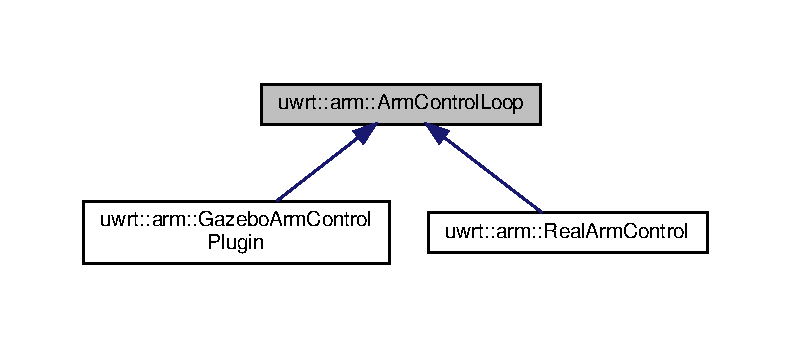
\includegraphics[width=350pt]{classuwrt_1_1arm_1_1_arm_control_loop__inherit__graph}
\end{center}
\end{figure}
\subsection*{Public Member Functions}
\begin{DoxyCompactItemize}
\item 
\hyperlink{classuwrt_1_1arm_1_1_arm_control_loop_a205726d352abb0e7696c10e337db0347}{Arm\+Control\+Loop} (std\+::string name, const ros\+::\+Node\+Handle \&nh=ros\+::\+Node\+Handle())
\begin{DoxyCompactList}\small\item\em Constructor. \end{DoxyCompactList}\item 
virtual \hyperlink{classuwrt_1_1arm_1_1_arm_control_loop_a35e34c53f7a7d42bc430e1b8a26328ee}{$\sim$\+Arm\+Control\+Loop} ()=default
\begin{DoxyCompactList}\small\item\em Destructor. \end{DoxyCompactList}\item 
virtual bool \hyperlink{classuwrt_1_1arm_1_1_arm_control_loop_a40fbe9c3e41bd01174c61aca2faec58b}{init} ()
\begin{DoxyCompactList}\small\item\em Initializer for the class. \end{DoxyCompactList}\item 
void \hyperlink{classuwrt_1_1arm_1_1_arm_control_loop_a3f779ad43e5c210bf977469d25f15036}{update} (const ros\+::\+Time \&time\+\_\+now, bool update\+\_\+controllers=true)
\begin{DoxyCompactList}\small\item\em Performs reads/writes and updates controllers. \end{DoxyCompactList}\end{DoxyCompactItemize}
\subsection*{Protected Attributes}
\begin{DoxyCompactItemize}
\item 
const std\+::string \hyperlink{classuwrt_1_1arm_1_1_arm_control_loop_a6082448e453dda1b08d3af23e156b889}{name\+\_\+}
\begin{DoxyCompactList}\small\item\em Name of the control loop object. \end{DoxyCompactList}\item 
ros\+::\+Node\+Handle \hyperlink{classuwrt_1_1arm_1_1_arm_control_loop_ac893531965c914e8ed54dfe97909be7d}{nh\+\_\+}
\begin{DoxyCompactList}\small\item\em Nodehandle. \end{DoxyCompactList}\item 
std\+::unique\+\_\+ptr$<$ \hyperlink{classuwrt_1_1arm_1_1_arm_h_w}{Arm\+HW} $>$ \hyperlink{classuwrt_1_1arm_1_1_arm_control_loop_ae28be35b3cf089ea2640f1104742cc32}{arm\+\_\+hw\+\_\+}
\begin{DoxyCompactList}\small\item\em Pointer to the hardware interface for the Arm $\ast$/. \end{DoxyCompactList}\item 
std\+::unique\+\_\+ptr$<$ controller\+\_\+manager\+::\+Controller\+Manager $>$ \hyperlink{classuwrt_1_1arm_1_1_arm_control_loop_a06f6565117c5a6052b09c1c41e9daba8}{controller\+\_\+manager\+\_\+}
\begin{DoxyCompactList}\small\item\em Manages all active and inactive controllers $\ast$/. \end{DoxyCompactList}\item 
ros\+::\+Time \hyperlink{classuwrt_1_1arm_1_1_arm_control_loop_aa9847f51f9c32be800979ac9422ba3b3}{last\+\_\+update\+\_\+time\+\_\+}
\begin{DoxyCompactList}\small\item\em The last time the controller manager updated the state of the controllers. \end{DoxyCompactList}\item 
ros\+::\+Time \hyperlink{classuwrt_1_1arm_1_1_arm_control_loop_a91b726de7d1791a6efedfaaa31344dea}{last\+\_\+rw\+\_\+time\+\_\+}
\begin{DoxyCompactList}\small\item\em The last time data was read from or written to the hardware interface. \end{DoxyCompactList}\item 
double \hyperlink{classuwrt_1_1arm_1_1_arm_control_loop_a28d7faaababb37ce0ffbb705ffe4fe0a}{controller\+\_\+watchdog\+\_\+timeout\+\_\+}
\begin{DoxyCompactList}\small\item\em Watchdog timer timeout for the active controller(s) \end{DoxyCompactList}\item 
double \hyperlink{classuwrt_1_1arm_1_1_arm_control_loop_a8c03c0b16204b0a38c1233ba0ea6ad0e}{control\+\_\+freq\+\_\+}
\begin{DoxyCompactList}\small\item\em Frequency of controller updates. \end{DoxyCompactList}\end{DoxyCompactItemize}


\subsection{Detailed Description}
Base class for Arm control loops that perform reads, writes and updates of controllers 

\subsection{Constructor \& Destructor Documentation}
\mbox{\Hypertarget{classuwrt_1_1arm_1_1_arm_control_loop_a205726d352abb0e7696c10e337db0347}\label{classuwrt_1_1arm_1_1_arm_control_loop_a205726d352abb0e7696c10e337db0347}} 
\index{uwrt\+::arm\+::\+Arm\+Control\+Loop@{uwrt\+::arm\+::\+Arm\+Control\+Loop}!Arm\+Control\+Loop@{Arm\+Control\+Loop}}
\index{Arm\+Control\+Loop@{Arm\+Control\+Loop}!uwrt\+::arm\+::\+Arm\+Control\+Loop@{uwrt\+::arm\+::\+Arm\+Control\+Loop}}
\subsubsection{\texorpdfstring{Arm\+Control\+Loop()}{ArmControlLoop()}}
{\footnotesize\ttfamily uwrt\+::arm\+::\+Arm\+Control\+Loop\+::\+Arm\+Control\+Loop (\begin{DoxyParamCaption}\item[{std\+::string}]{name,  }\item[{const ros\+::\+Node\+Handle \&}]{nh = {\ttfamily ros\+:\+:NodeHandle()} }\end{DoxyParamCaption})}



Constructor. 


\begin{DoxyParams}{Parameters}
{\em name} & Name for the \hyperlink{classuwrt_1_1arm_1_1_arm_control_loop}{Arm\+Control\+Loop} object \\
\hline
{\em nh} & R\+OS Nodehandle for root of the arm namespace \\
\hline
\end{DoxyParams}
\mbox{\Hypertarget{classuwrt_1_1arm_1_1_arm_control_loop_a35e34c53f7a7d42bc430e1b8a26328ee}\label{classuwrt_1_1arm_1_1_arm_control_loop_a35e34c53f7a7d42bc430e1b8a26328ee}} 
\index{uwrt\+::arm\+::\+Arm\+Control\+Loop@{uwrt\+::arm\+::\+Arm\+Control\+Loop}!````~Arm\+Control\+Loop@{$\sim$\+Arm\+Control\+Loop}}
\index{````~Arm\+Control\+Loop@{$\sim$\+Arm\+Control\+Loop}!uwrt\+::arm\+::\+Arm\+Control\+Loop@{uwrt\+::arm\+::\+Arm\+Control\+Loop}}
\subsubsection{\texorpdfstring{$\sim$\+Arm\+Control\+Loop()}{~ArmControlLoop()}}
{\footnotesize\ttfamily virtual uwrt\+::arm\+::\+Arm\+Control\+Loop\+::$\sim$\+Arm\+Control\+Loop (\begin{DoxyParamCaption}{ }\end{DoxyParamCaption})\hspace{0.3cm}{\ttfamily [virtual]}, {\ttfamily [default]}}



Destructor. 



\subsection{Member Function Documentation}
\mbox{\Hypertarget{classuwrt_1_1arm_1_1_arm_control_loop_a40fbe9c3e41bd01174c61aca2faec58b}\label{classuwrt_1_1arm_1_1_arm_control_loop_a40fbe9c3e41bd01174c61aca2faec58b}} 
\index{uwrt\+::arm\+::\+Arm\+Control\+Loop@{uwrt\+::arm\+::\+Arm\+Control\+Loop}!init@{init}}
\index{init@{init}!uwrt\+::arm\+::\+Arm\+Control\+Loop@{uwrt\+::arm\+::\+Arm\+Control\+Loop}}
\subsubsection{\texorpdfstring{init()}{init()}}
{\footnotesize\ttfamily bool uwrt\+::arm\+::\+Arm\+Control\+Loop\+::init (\begin{DoxyParamCaption}{ }\end{DoxyParamCaption})\hspace{0.3cm}{\ttfamily [virtual]}}



Initializer for the class. 

\mbox{\Hypertarget{classuwrt_1_1arm_1_1_arm_control_loop_a3f779ad43e5c210bf977469d25f15036}\label{classuwrt_1_1arm_1_1_arm_control_loop_a3f779ad43e5c210bf977469d25f15036}} 
\index{uwrt\+::arm\+::\+Arm\+Control\+Loop@{uwrt\+::arm\+::\+Arm\+Control\+Loop}!update@{update}}
\index{update@{update}!uwrt\+::arm\+::\+Arm\+Control\+Loop@{uwrt\+::arm\+::\+Arm\+Control\+Loop}}
\subsubsection{\texorpdfstring{update()}{update()}}
{\footnotesize\ttfamily void uwrt\+::arm\+::\+Arm\+Control\+Loop\+::update (\begin{DoxyParamCaption}\item[{const ros\+::\+Time \&}]{time\+\_\+now,  }\item[{bool}]{update\+\_\+controllers = {\ttfamily true} }\end{DoxyParamCaption})}



Performs reads/writes and updates controllers. 

Reads and writes to the hardware are performed at each call to this function. The controller manager updates the state of the controllers when specified


\begin{DoxyParams}{Parameters}
{\em time\+\_\+now} & The current R\+OS time \\
\hline
{\em update\+\_\+controllers} & Whether to update the controller states (e.\+g. start, stop, switch, etc) \\
\hline
\end{DoxyParams}


\subsection{Member Data Documentation}
\mbox{\Hypertarget{classuwrt_1_1arm_1_1_arm_control_loop_ae28be35b3cf089ea2640f1104742cc32}\label{classuwrt_1_1arm_1_1_arm_control_loop_ae28be35b3cf089ea2640f1104742cc32}} 
\index{uwrt\+::arm\+::\+Arm\+Control\+Loop@{uwrt\+::arm\+::\+Arm\+Control\+Loop}!arm\+\_\+hw\+\_\+@{arm\+\_\+hw\+\_\+}}
\index{arm\+\_\+hw\+\_\+@{arm\+\_\+hw\+\_\+}!uwrt\+::arm\+::\+Arm\+Control\+Loop@{uwrt\+::arm\+::\+Arm\+Control\+Loop}}
\subsubsection{\texorpdfstring{arm\+\_\+hw\+\_\+}{arm\_hw\_}}
{\footnotesize\ttfamily std\+::unique\+\_\+ptr$<$\hyperlink{classuwrt_1_1arm_1_1_arm_h_w}{Arm\+HW}$>$ uwrt\+::arm\+::\+Arm\+Control\+Loop\+::arm\+\_\+hw\+\_\+\hspace{0.3cm}{\ttfamily [protected]}}



Pointer to the hardware interface for the Arm $\ast$/. 

\mbox{\Hypertarget{classuwrt_1_1arm_1_1_arm_control_loop_a8c03c0b16204b0a38c1233ba0ea6ad0e}\label{classuwrt_1_1arm_1_1_arm_control_loop_a8c03c0b16204b0a38c1233ba0ea6ad0e}} 
\index{uwrt\+::arm\+::\+Arm\+Control\+Loop@{uwrt\+::arm\+::\+Arm\+Control\+Loop}!control\+\_\+freq\+\_\+@{control\+\_\+freq\+\_\+}}
\index{control\+\_\+freq\+\_\+@{control\+\_\+freq\+\_\+}!uwrt\+::arm\+::\+Arm\+Control\+Loop@{uwrt\+::arm\+::\+Arm\+Control\+Loop}}
\subsubsection{\texorpdfstring{control\+\_\+freq\+\_\+}{control\_freq\_}}
{\footnotesize\ttfamily double uwrt\+::arm\+::\+Arm\+Control\+Loop\+::control\+\_\+freq\+\_\+\hspace{0.3cm}{\ttfamily [protected]}}



Frequency of controller updates. 

\mbox{\Hypertarget{classuwrt_1_1arm_1_1_arm_control_loop_a06f6565117c5a6052b09c1c41e9daba8}\label{classuwrt_1_1arm_1_1_arm_control_loop_a06f6565117c5a6052b09c1c41e9daba8}} 
\index{uwrt\+::arm\+::\+Arm\+Control\+Loop@{uwrt\+::arm\+::\+Arm\+Control\+Loop}!controller\+\_\+manager\+\_\+@{controller\+\_\+manager\+\_\+}}
\index{controller\+\_\+manager\+\_\+@{controller\+\_\+manager\+\_\+}!uwrt\+::arm\+::\+Arm\+Control\+Loop@{uwrt\+::arm\+::\+Arm\+Control\+Loop}}
\subsubsection{\texorpdfstring{controller\+\_\+manager\+\_\+}{controller\_manager\_}}
{\footnotesize\ttfamily std\+::unique\+\_\+ptr$<$controller\+\_\+manager\+::\+Controller\+Manager$>$ uwrt\+::arm\+::\+Arm\+Control\+Loop\+::controller\+\_\+manager\+\_\+\hspace{0.3cm}{\ttfamily [protected]}}



Manages all active and inactive controllers $\ast$/. 

\mbox{\Hypertarget{classuwrt_1_1arm_1_1_arm_control_loop_a28d7faaababb37ce0ffbb705ffe4fe0a}\label{classuwrt_1_1arm_1_1_arm_control_loop_a28d7faaababb37ce0ffbb705ffe4fe0a}} 
\index{uwrt\+::arm\+::\+Arm\+Control\+Loop@{uwrt\+::arm\+::\+Arm\+Control\+Loop}!controller\+\_\+watchdog\+\_\+timeout\+\_\+@{controller\+\_\+watchdog\+\_\+timeout\+\_\+}}
\index{controller\+\_\+watchdog\+\_\+timeout\+\_\+@{controller\+\_\+watchdog\+\_\+timeout\+\_\+}!uwrt\+::arm\+::\+Arm\+Control\+Loop@{uwrt\+::arm\+::\+Arm\+Control\+Loop}}
\subsubsection{\texorpdfstring{controller\+\_\+watchdog\+\_\+timeout\+\_\+}{controller\_watchdog\_timeout\_}}
{\footnotesize\ttfamily double uwrt\+::arm\+::\+Arm\+Control\+Loop\+::controller\+\_\+watchdog\+\_\+timeout\+\_\+\hspace{0.3cm}{\ttfamily [protected]}}



Watchdog timer timeout for the active controller(s) 

\mbox{\Hypertarget{classuwrt_1_1arm_1_1_arm_control_loop_a91b726de7d1791a6efedfaaa31344dea}\label{classuwrt_1_1arm_1_1_arm_control_loop_a91b726de7d1791a6efedfaaa31344dea}} 
\index{uwrt\+::arm\+::\+Arm\+Control\+Loop@{uwrt\+::arm\+::\+Arm\+Control\+Loop}!last\+\_\+rw\+\_\+time\+\_\+@{last\+\_\+rw\+\_\+time\+\_\+}}
\index{last\+\_\+rw\+\_\+time\+\_\+@{last\+\_\+rw\+\_\+time\+\_\+}!uwrt\+::arm\+::\+Arm\+Control\+Loop@{uwrt\+::arm\+::\+Arm\+Control\+Loop}}
\subsubsection{\texorpdfstring{last\+\_\+rw\+\_\+time\+\_\+}{last\_rw\_time\_}}
{\footnotesize\ttfamily ros\+::\+Time uwrt\+::arm\+::\+Arm\+Control\+Loop\+::last\+\_\+rw\+\_\+time\+\_\+\hspace{0.3cm}{\ttfamily [protected]}}



The last time data was read from or written to the hardware interface. 

\mbox{\Hypertarget{classuwrt_1_1arm_1_1_arm_control_loop_aa9847f51f9c32be800979ac9422ba3b3}\label{classuwrt_1_1arm_1_1_arm_control_loop_aa9847f51f9c32be800979ac9422ba3b3}} 
\index{uwrt\+::arm\+::\+Arm\+Control\+Loop@{uwrt\+::arm\+::\+Arm\+Control\+Loop}!last\+\_\+update\+\_\+time\+\_\+@{last\+\_\+update\+\_\+time\+\_\+}}
\index{last\+\_\+update\+\_\+time\+\_\+@{last\+\_\+update\+\_\+time\+\_\+}!uwrt\+::arm\+::\+Arm\+Control\+Loop@{uwrt\+::arm\+::\+Arm\+Control\+Loop}}
\subsubsection{\texorpdfstring{last\+\_\+update\+\_\+time\+\_\+}{last\_update\_time\_}}
{\footnotesize\ttfamily ros\+::\+Time uwrt\+::arm\+::\+Arm\+Control\+Loop\+::last\+\_\+update\+\_\+time\+\_\+\hspace{0.3cm}{\ttfamily [protected]}}



The last time the controller manager updated the state of the controllers. 

\mbox{\Hypertarget{classuwrt_1_1arm_1_1_arm_control_loop_a6082448e453dda1b08d3af23e156b889}\label{classuwrt_1_1arm_1_1_arm_control_loop_a6082448e453dda1b08d3af23e156b889}} 
\index{uwrt\+::arm\+::\+Arm\+Control\+Loop@{uwrt\+::arm\+::\+Arm\+Control\+Loop}!name\+\_\+@{name\+\_\+}}
\index{name\+\_\+@{name\+\_\+}!uwrt\+::arm\+::\+Arm\+Control\+Loop@{uwrt\+::arm\+::\+Arm\+Control\+Loop}}
\subsubsection{\texorpdfstring{name\+\_\+}{name\_}}
{\footnotesize\ttfamily const std\+::string uwrt\+::arm\+::\+Arm\+Control\+Loop\+::name\+\_\+\hspace{0.3cm}{\ttfamily [protected]}}



Name of the control loop object. 

\mbox{\Hypertarget{classuwrt_1_1arm_1_1_arm_control_loop_ac893531965c914e8ed54dfe97909be7d}\label{classuwrt_1_1arm_1_1_arm_control_loop_ac893531965c914e8ed54dfe97909be7d}} 
\index{uwrt\+::arm\+::\+Arm\+Control\+Loop@{uwrt\+::arm\+::\+Arm\+Control\+Loop}!nh\+\_\+@{nh\+\_\+}}
\index{nh\+\_\+@{nh\+\_\+}!uwrt\+::arm\+::\+Arm\+Control\+Loop@{uwrt\+::arm\+::\+Arm\+Control\+Loop}}
\subsubsection{\texorpdfstring{nh\+\_\+}{nh\_}}
{\footnotesize\ttfamily ros\+::\+Node\+Handle uwrt\+::arm\+::\+Arm\+Control\+Loop\+::nh\+\_\+\hspace{0.3cm}{\ttfamily [protected]}}



Nodehandle. 



The documentation for this class was generated from the following files\+:\begin{DoxyCompactItemize}
\item 
uwrt\+\_\+arm\+\_\+hw/include/uwrt\+\_\+arm\+\_\+hw/\hyperlink{arm__control__loop_8h}{arm\+\_\+control\+\_\+loop.\+h}\item 
uwrt\+\_\+arm\+\_\+hw/src/\hyperlink{arm__control__loop_8cpp}{arm\+\_\+control\+\_\+loop.\+cpp}\end{DoxyCompactItemize}

\hypertarget{classuwrt_1_1arm_1_1_arm_h_w}{}\section{uwrt\+:\+:arm\+:\+:Arm\+HW Class Reference}
\label{classuwrt_1_1arm_1_1_arm_h_w}\index{uwrt\+::arm\+::\+Arm\+HW@{uwrt\+::arm\+::\+Arm\+HW}}


{\ttfamily \#include $<$arm\+\_\+hw.\+h$>$}



Inheritance diagram for uwrt\+:\+:arm\+:\+:Arm\+HW\+:
\nopagebreak
\begin{figure}[H]
\begin{center}
\leavevmode
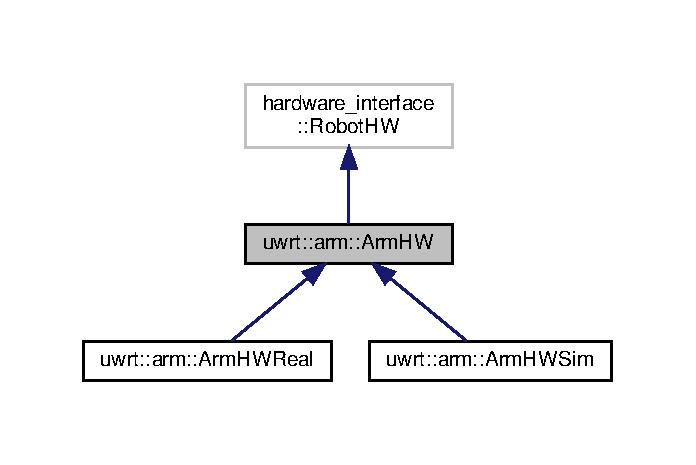
\includegraphics[width=334pt]{classuwrt_1_1arm_1_1_arm_h_w__inherit__graph}
\end{center}
\end{figure}


Collaboration diagram for uwrt\+:\+:arm\+:\+:Arm\+HW\+:
\nopagebreak
\begin{figure}[H]
\begin{center}
\leavevmode
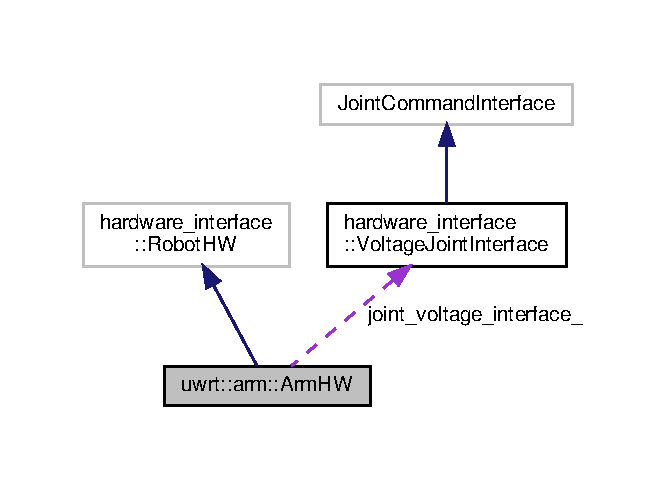
\includegraphics[width=320pt]{classuwrt_1_1arm_1_1_arm_h_w__coll__graph}
\end{center}
\end{figure}
\subsection*{Public Member Functions}
\begin{DoxyCompactItemize}
\item 
\hyperlink{classuwrt_1_1arm_1_1_arm_h_w_a715621a4a3f913beac7d6e4f16b40c11}{Arm\+HW} (const std\+::string \&urdf\+\_\+str)
\begin{DoxyCompactList}\small\item\em Constructor. \end{DoxyCompactList}\item 
\hyperlink{classuwrt_1_1arm_1_1_arm_h_w_a03495dca1c1616fb09184541713f0670}{Arm\+HW} (const std\+::string \&name, const std\+::string \&urdf\+\_\+str)
\begin{DoxyCompactList}\small\item\em \+: Constructor \end{DoxyCompactList}\item 
bool \hyperlink{classuwrt_1_1arm_1_1_arm_h_w_a2b8c89b8498c70d8b627fefd17267e40}{init} (ros\+::\+Node\+Handle \&nh, ros\+::\+Node\+Handle \&arm\+\_\+hw\+\_\+nh) override
\begin{DoxyCompactList}\small\item\em Initializes the hardware interface by registering all joints and interfaces. \end{DoxyCompactList}\item 
void \hyperlink{classuwrt_1_1arm_1_1_arm_h_w_ae5bbb33ef19c7e27fa0e3888fda5b372}{do\+Switch} (const std\+::list$<$ hardware\+\_\+interface\+::\+Controller\+Info $>$ \&start\+\_\+list, const std\+::list$<$ hardware\+\_\+interface\+::\+Controller\+Info $>$ \&stop\+\_\+list) override
\begin{DoxyCompactList}\small\item\em Starts/\+Stops controllers based on controller manager service calls. \end{DoxyCompactList}\item 
virtual void \hyperlink{classuwrt_1_1arm_1_1_arm_h_w_af2164103badfa99373f787b8a3cecb6b}{read} (const ros\+::\+Time \&time, const ros\+::\+Duration \&period)=0
\begin{DoxyCompactList}\small\item\em Reads data from the arm. \end{DoxyCompactList}\item 
virtual void \hyperlink{classuwrt_1_1arm_1_1_arm_h_w_a934119487836109e24d9054f10e9832f}{write} (const ros\+::\+Time \&time, const ros\+::\+Duration \&period)=0
\begin{DoxyCompactList}\small\item\em Writes data to the arm. \end{DoxyCompactList}\item 
void \hyperlink{classuwrt_1_1arm_1_1_arm_h_w_aef2643b05e4070ab7142eca2be62ddd1}{enforce\+Limits} (ros\+::\+Duration period)
\begin{DoxyCompactList}\small\item\em Enforces predefined limits on controller outputs. \end{DoxyCompactList}\item 
std\+::string \hyperlink{classuwrt_1_1arm_1_1_arm_h_w_a2ded1550eac19e0ea4ac4830fe196ad5}{get\+Name} () const
\begin{DoxyCompactList}\small\item\em Get the name of the hardware interface object. \end{DoxyCompactList}\end{DoxyCompactItemize}
\subsection*{Protected Types}
\begin{DoxyCompactItemize}
\item 
enum \hyperlink{classuwrt_1_1arm_1_1_arm_h_w_aef42f10e04f7f426b3d06f91d0897b6b}{Control\+Method} \{ \hyperlink{classuwrt_1_1arm_1_1_arm_h_w_aef42f10e04f7f426b3d06f91d0897b6ba7e141378d3029e25ce86b40cc794e8d6}{P\+O\+S\+I\+T\+I\+ON}, 
\hyperlink{classuwrt_1_1arm_1_1_arm_h_w_aef42f10e04f7f426b3d06f91d0897b6ba143f6d42adf4ed0f7b4f776bac5fc645}{V\+E\+L\+O\+C\+I\+TY}, 
\hyperlink{classuwrt_1_1arm_1_1_arm_h_w_aef42f10e04f7f426b3d06f91d0897b6ba5de839ecc8d975a1ebb795e0439e1904}{E\+F\+F\+O\+RT}, 
\hyperlink{classuwrt_1_1arm_1_1_arm_h_w_aef42f10e04f7f426b3d06f91d0897b6ba0ba2d8d7f2e958362c284ffbcf7a686f}{V\+O\+L\+T\+A\+GE}
 \}\begin{DoxyCompactList}\small\item\em Enum for the mode of control for a joint. \end{DoxyCompactList}
\end{DoxyCompactItemize}
\subsection*{Protected Attributes}
\begin{DoxyCompactItemize}
\item 
ros\+::\+Node\+Handle \hyperlink{classuwrt_1_1arm_1_1_arm_h_w_a80bff071cccf662191970b5088619a29}{nh\+\_\+}
\item 
ros\+::\+Node\+Handle \hyperlink{classuwrt_1_1arm_1_1_arm_h_w_a47b8fb1ffec74c5699b3d32827b4f5b6}{arm\+\_\+hw\+\_\+nh\+\_\+}
\item 
const std\+::string \hyperlink{classuwrt_1_1arm_1_1_arm_h_w_a94577174f3c73549997c501acb28810a}{name\+\_\+}
\item 
const std\+::string \hyperlink{classuwrt_1_1arm_1_1_arm_h_w_a0708e51d21f05e20129b7bc99e42eead}{urdf\+\_\+string\+\_\+}
\item 
urdf\+::\+Model \hyperlink{classuwrt_1_1arm_1_1_arm_h_w_a356557f068878c9464f4d47eb6381ae3}{urdf\+\_\+model\+\_\+}
\item 
const int8\+\_\+t \hyperlink{classuwrt_1_1arm_1_1_arm_h_w_ab1263af2b5e65e88876efdb45025080c}{num\+\_\+joints\+\_\+}
\item 
std\+::vector$<$ std\+::string $>$ \hyperlink{classuwrt_1_1arm_1_1_arm_h_w_a0bba123f549c158be6dbfc365e42853d}{joint\+\_\+names\+\_\+}
\item 
std\+::vector$<$ double $>$ \hyperlink{classuwrt_1_1arm_1_1_arm_h_w_a08c5d50dddb1a3552b43bfff0d07ffa9}{joint\+\_\+lower\+\_\+limits\+\_\+}
\item 
std\+::vector$<$ double $>$ \hyperlink{classuwrt_1_1arm_1_1_arm_h_w_a4073badaad21458259a93fb66f510a9e}{joint\+\_\+upper\+\_\+limits\+\_\+}
\item 
std\+::vector$<$ double $>$ \hyperlink{classuwrt_1_1arm_1_1_arm_h_w_ab6f08fdf70a33a99af148bc5ce0f56ad}{joint\+\_\+effort\+\_\+limits\+\_\+}
\item 
std\+::vector$<$ double $>$ \hyperlink{classuwrt_1_1arm_1_1_arm_h_w_ac6612898a4add151094f92b87cc8ded7}{joint\+\_\+position\+\_\+}
\item 
std\+::vector$<$ double $>$ \hyperlink{classuwrt_1_1arm_1_1_arm_h_w_ab7b253782896e1bc6a1879dcbae60c47}{joint\+\_\+position\+\_\+command\+\_\+}
\item 
std\+::vector$<$ double $>$ \hyperlink{classuwrt_1_1arm_1_1_arm_h_w_abbf5caed643c4c897c4bf5a0c209bff7}{joint\+\_\+velocity\+\_\+}
\item 
std\+::vector$<$ double $>$ \hyperlink{classuwrt_1_1arm_1_1_arm_h_w_aa4acfb5b9cf32153470bc9e384e2fb85}{joint\+\_\+velocity\+\_\+command\+\_\+}
\item 
std\+::vector$<$ double $>$ \hyperlink{classuwrt_1_1arm_1_1_arm_h_w_aed887286b800a8852217146876a9bb6b}{joint\+\_\+effort\+\_\+}
\item 
std\+::vector$<$ double $>$ \hyperlink{classuwrt_1_1arm_1_1_arm_h_w_a9e0792faa7682cd234cfa518e976e79c}{joint\+\_\+effort\+\_\+command\+\_\+}
\item 
std\+::vector$<$ double $>$ \hyperlink{classuwrt_1_1arm_1_1_arm_h_w_acaa46956d8f97421c96c9b5a9b51200f}{joint\+\_\+voltage\+\_\+command\+\_\+}
\item 
std\+::vector$<$ \hyperlink{classuwrt_1_1arm_1_1_arm_h_w_aef42f10e04f7f426b3d06f91d0897b6b}{Control\+Method} $>$ \hyperlink{classuwrt_1_1arm_1_1_arm_h_w_ad19ee0c5fe04b8e8366f036010927fc4}{joint\+\_\+control\+\_\+method\+\_\+}
\item 
std\+::map$<$ std\+::string, uint8\+\_\+t $>$ \hyperlink{classuwrt_1_1arm_1_1_arm_h_w_afec1b4685b242f4d7e821f6e6c479302}{joint\+\_\+index\+\_\+map\+\_\+}
\begin{DoxyCompactList}\small\item\em Mapping from joint name to an index. \end{DoxyCompactList}\item 
std\+::vector$<$ int $>$ \hyperlink{classuwrt_1_1arm_1_1_arm_h_w_a69c250992873f9451b2d0e45fb1fc41e}{joint\+\_\+types\+\_\+}
\item 
hardware\+\_\+interface\+::\+Joint\+State\+Interface \hyperlink{classuwrt_1_1arm_1_1_arm_h_w_af7b1df1eb7f6e3badcc369be49af7978}{joint\+\_\+state\+\_\+interface\+\_\+}
\item 
hardware\+\_\+interface\+::\+Position\+Joint\+Interface \hyperlink{classuwrt_1_1arm_1_1_arm_h_w_ac0e4f2bbeaac8437cafa891602a7e0a0}{joint\+\_\+position\+\_\+interface\+\_\+}
\item 
hardware\+\_\+interface\+::\+Velocity\+Joint\+Interface \hyperlink{classuwrt_1_1arm_1_1_arm_h_w_af0a297190b6a67aee4f86fb7f44c36d2}{joint\+\_\+velocity\+\_\+interface\+\_\+}
\item 
hardware\+\_\+interface\+::\+Effort\+Joint\+Interface \hyperlink{classuwrt_1_1arm_1_1_arm_h_w_a5d2464c0da77d58da43af0baa5d7c2a4}{joint\+\_\+effort\+\_\+interface\+\_\+}
\item 
\hyperlink{classhardware__interface_1_1_voltage_joint_interface}{hardware\+\_\+interface\+::\+Voltage\+Joint\+Interface} \hyperlink{classuwrt_1_1arm_1_1_arm_h_w_aec35c81c5c9a7f32fe38ea3cdfbb8b6d}{joint\+\_\+voltage\+\_\+interface\+\_\+}
\item 
joint\+\_\+limits\+\_\+interface\+::\+Position\+Joint\+Saturation\+Interface \hyperlink{classuwrt_1_1arm_1_1_arm_h_w_ad940f7d5b2561be5ff6c3350480e20b5}{position\+\_\+sat\+\_\+interface\+\_\+}
\item 
joint\+\_\+limits\+\_\+interface\+::\+Position\+Joint\+Soft\+Limits\+Interface \hyperlink{classuwrt_1_1arm_1_1_arm_h_w_a84a73ead7105311112f7fe8ae7eda096}{position\+\_\+limits\+\_\+interface\+\_\+}
\item 
joint\+\_\+limits\+\_\+interface\+::\+Velocity\+Joint\+Saturation\+Interface \hyperlink{classuwrt_1_1arm_1_1_arm_h_w_a461fd5b0255bf2d1eecfb384ff7f1987}{velocity\+\_\+sat\+\_\+interface\+\_\+}
\item 
joint\+\_\+limits\+\_\+interface\+::\+Velocity\+Joint\+Soft\+Limits\+Interface \hyperlink{classuwrt_1_1arm_1_1_arm_h_w_a8e2811fbe4adfcbcce9efbee3756ea8f}{velocity\+\_\+limits\+\_\+interface\+\_\+}
\item 
joint\+\_\+limits\+\_\+interface\+::\+Effort\+Joint\+Saturation\+Interface \hyperlink{classuwrt_1_1arm_1_1_arm_h_w_a6272ed655471405069584b1afd4de5a7}{effort\+\_\+sat\+\_\+interface\+\_\+}
\item 
joint\+\_\+limits\+\_\+interface\+::\+Effort\+Joint\+Soft\+Limits\+Interface \hyperlink{classuwrt_1_1arm_1_1_arm_h_w_ac1add3b1c8d7423339d24de09a706485}{effort\+\_\+limits\+\_\+interface\+\_\+}
\end{DoxyCompactItemize}


\subsection{Detailed Description}
Base class for the Arm hardware interface required by ros\+\_\+control 

\subsection{Member Enumeration Documentation}
\mbox{\Hypertarget{classuwrt_1_1arm_1_1_arm_h_w_aef42f10e04f7f426b3d06f91d0897b6b}\label{classuwrt_1_1arm_1_1_arm_h_w_aef42f10e04f7f426b3d06f91d0897b6b}} 
\index{uwrt\+::arm\+::\+Arm\+HW@{uwrt\+::arm\+::\+Arm\+HW}!Control\+Method@{Control\+Method}}
\index{Control\+Method@{Control\+Method}!uwrt\+::arm\+::\+Arm\+HW@{uwrt\+::arm\+::\+Arm\+HW}}
\subsubsection{\texorpdfstring{Control\+Method}{ControlMethod}}
{\footnotesize\ttfamily enum \hyperlink{classuwrt_1_1arm_1_1_arm_h_w_aef42f10e04f7f426b3d06f91d0897b6b}{uwrt\+::arm\+::\+Arm\+H\+W\+::\+Control\+Method}\hspace{0.3cm}{\ttfamily [protected]}}



Enum for the mode of control for a joint. 

\begin{DoxyEnumFields}{Enumerator}
\raisebox{\heightof{T}}[0pt][0pt]{\index{P\+O\+S\+I\+T\+I\+ON@{P\+O\+S\+I\+T\+I\+ON}!uwrt\+::arm\+::\+Arm\+HW@{uwrt\+::arm\+::\+Arm\+HW}}\index{uwrt\+::arm\+::\+Arm\+HW@{uwrt\+::arm\+::\+Arm\+HW}!P\+O\+S\+I\+T\+I\+ON@{P\+O\+S\+I\+T\+I\+ON}}}\mbox{\Hypertarget{classuwrt_1_1arm_1_1_arm_h_w_aef42f10e04f7f426b3d06f91d0897b6ba7e141378d3029e25ce86b40cc794e8d6}\label{classuwrt_1_1arm_1_1_arm_h_w_aef42f10e04f7f426b3d06f91d0897b6ba7e141378d3029e25ce86b40cc794e8d6}} 
P\+O\+S\+I\+T\+I\+ON&\\
\hline

\raisebox{\heightof{T}}[0pt][0pt]{\index{V\+E\+L\+O\+C\+I\+TY@{V\+E\+L\+O\+C\+I\+TY}!uwrt\+::arm\+::\+Arm\+HW@{uwrt\+::arm\+::\+Arm\+HW}}\index{uwrt\+::arm\+::\+Arm\+HW@{uwrt\+::arm\+::\+Arm\+HW}!V\+E\+L\+O\+C\+I\+TY@{V\+E\+L\+O\+C\+I\+TY}}}\mbox{\Hypertarget{classuwrt_1_1arm_1_1_arm_h_w_aef42f10e04f7f426b3d06f91d0897b6ba143f6d42adf4ed0f7b4f776bac5fc645}\label{classuwrt_1_1arm_1_1_arm_h_w_aef42f10e04f7f426b3d06f91d0897b6ba143f6d42adf4ed0f7b4f776bac5fc645}} 
V\+E\+L\+O\+C\+I\+TY&\\
\hline

\raisebox{\heightof{T}}[0pt][0pt]{\index{E\+F\+F\+O\+RT@{E\+F\+F\+O\+RT}!uwrt\+::arm\+::\+Arm\+HW@{uwrt\+::arm\+::\+Arm\+HW}}\index{uwrt\+::arm\+::\+Arm\+HW@{uwrt\+::arm\+::\+Arm\+HW}!E\+F\+F\+O\+RT@{E\+F\+F\+O\+RT}}}\mbox{\Hypertarget{classuwrt_1_1arm_1_1_arm_h_w_aef42f10e04f7f426b3d06f91d0897b6ba5de839ecc8d975a1ebb795e0439e1904}\label{classuwrt_1_1arm_1_1_arm_h_w_aef42f10e04f7f426b3d06f91d0897b6ba5de839ecc8d975a1ebb795e0439e1904}} 
E\+F\+F\+O\+RT&\\
\hline

\raisebox{\heightof{T}}[0pt][0pt]{\index{V\+O\+L\+T\+A\+GE@{V\+O\+L\+T\+A\+GE}!uwrt\+::arm\+::\+Arm\+HW@{uwrt\+::arm\+::\+Arm\+HW}}\index{uwrt\+::arm\+::\+Arm\+HW@{uwrt\+::arm\+::\+Arm\+HW}!V\+O\+L\+T\+A\+GE@{V\+O\+L\+T\+A\+GE}}}\mbox{\Hypertarget{classuwrt_1_1arm_1_1_arm_h_w_aef42f10e04f7f426b3d06f91d0897b6ba0ba2d8d7f2e958362c284ffbcf7a686f}\label{classuwrt_1_1arm_1_1_arm_h_w_aef42f10e04f7f426b3d06f91d0897b6ba0ba2d8d7f2e958362c284ffbcf7a686f}} 
V\+O\+L\+T\+A\+GE&\\
\hline

\end{DoxyEnumFields}


\subsection{Constructor \& Destructor Documentation}
\mbox{\Hypertarget{classuwrt_1_1arm_1_1_arm_h_w_a715621a4a3f913beac7d6e4f16b40c11}\label{classuwrt_1_1arm_1_1_arm_h_w_a715621a4a3f913beac7d6e4f16b40c11}} 
\index{uwrt\+::arm\+::\+Arm\+HW@{uwrt\+::arm\+::\+Arm\+HW}!Arm\+HW@{Arm\+HW}}
\index{Arm\+HW@{Arm\+HW}!uwrt\+::arm\+::\+Arm\+HW@{uwrt\+::arm\+::\+Arm\+HW}}
\subsubsection{\texorpdfstring{Arm\+H\+W()}{ArmHW()}\hspace{0.1cm}{\footnotesize\ttfamily [1/2]}}
{\footnotesize\ttfamily uwrt\+::arm\+::\+Arm\+H\+W\+::\+Arm\+HW (\begin{DoxyParamCaption}\item[{const std\+::string \&}]{urdf\+\_\+str }\end{DoxyParamCaption})\hspace{0.3cm}{\ttfamily [explicit]}}



Constructor. 


\begin{DoxyParams}{Parameters}
{\em urdf\+\_\+str} & U\+R\+DF of the arm in string format \\
\hline
\end{DoxyParams}
\mbox{\Hypertarget{classuwrt_1_1arm_1_1_arm_h_w_a03495dca1c1616fb09184541713f0670}\label{classuwrt_1_1arm_1_1_arm_h_w_a03495dca1c1616fb09184541713f0670}} 
\index{uwrt\+::arm\+::\+Arm\+HW@{uwrt\+::arm\+::\+Arm\+HW}!Arm\+HW@{Arm\+HW}}
\index{Arm\+HW@{Arm\+HW}!uwrt\+::arm\+::\+Arm\+HW@{uwrt\+::arm\+::\+Arm\+HW}}
\subsubsection{\texorpdfstring{Arm\+H\+W()}{ArmHW()}\hspace{0.1cm}{\footnotesize\ttfamily [2/2]}}
{\footnotesize\ttfamily uwrt\+::arm\+::\+Arm\+H\+W\+::\+Arm\+HW (\begin{DoxyParamCaption}\item[{const std\+::string \&}]{name,  }\item[{const std\+::string \&}]{urdf\+\_\+str }\end{DoxyParamCaption})}



\+: Constructor 


\begin{DoxyParams}{Parameters}
{\em name} & Arbitrary name for an instance of this class \\
\hline
{\em urdf\+\_\+str} & U\+R\+DF of the arm in string format \\
\hline
\end{DoxyParams}


\subsection{Member Function Documentation}
\mbox{\Hypertarget{classuwrt_1_1arm_1_1_arm_h_w_ae5bbb33ef19c7e27fa0e3888fda5b372}\label{classuwrt_1_1arm_1_1_arm_h_w_ae5bbb33ef19c7e27fa0e3888fda5b372}} 
\index{uwrt\+::arm\+::\+Arm\+HW@{uwrt\+::arm\+::\+Arm\+HW}!do\+Switch@{do\+Switch}}
\index{do\+Switch@{do\+Switch}!uwrt\+::arm\+::\+Arm\+HW@{uwrt\+::arm\+::\+Arm\+HW}}
\subsubsection{\texorpdfstring{do\+Switch()}{doSwitch()}}
{\footnotesize\ttfamily void uwrt\+::arm\+::\+Arm\+H\+W\+::do\+Switch (\begin{DoxyParamCaption}\item[{const std\+::list$<$ hardware\+\_\+interface\+::\+Controller\+Info $>$ \&}]{start\+\_\+list,  }\item[{const std\+::list$<$ hardware\+\_\+interface\+::\+Controller\+Info $>$ \&}]{stop\+\_\+list }\end{DoxyParamCaption})\hspace{0.3cm}{\ttfamily [override]}}



Starts/\+Stops controllers based on controller manager service calls. 


\begin{DoxyParams}{Parameters}
{\em start\+\_\+list} & Controllers to start \\
\hline
{\em stop\+\_\+list} & Controllers to stop \\
\hline
\end{DoxyParams}
\mbox{\Hypertarget{classuwrt_1_1arm_1_1_arm_h_w_aef2643b05e4070ab7142eca2be62ddd1}\label{classuwrt_1_1arm_1_1_arm_h_w_aef2643b05e4070ab7142eca2be62ddd1}} 
\index{uwrt\+::arm\+::\+Arm\+HW@{uwrt\+::arm\+::\+Arm\+HW}!enforce\+Limits@{enforce\+Limits}}
\index{enforce\+Limits@{enforce\+Limits}!uwrt\+::arm\+::\+Arm\+HW@{uwrt\+::arm\+::\+Arm\+HW}}
\subsubsection{\texorpdfstring{enforce\+Limits()}{enforceLimits()}}
{\footnotesize\ttfamily void uwrt\+::arm\+::\+Arm\+H\+W\+::enforce\+Limits (\begin{DoxyParamCaption}\item[{ros\+::\+Duration}]{period }\end{DoxyParamCaption})}



Enforces predefined limits on controller outputs. 


\begin{DoxyParams}{Parameters}
{\em period} & Control period \\
\hline
\end{DoxyParams}
\mbox{\Hypertarget{classuwrt_1_1arm_1_1_arm_h_w_a2ded1550eac19e0ea4ac4830fe196ad5}\label{classuwrt_1_1arm_1_1_arm_h_w_a2ded1550eac19e0ea4ac4830fe196ad5}} 
\index{uwrt\+::arm\+::\+Arm\+HW@{uwrt\+::arm\+::\+Arm\+HW}!get\+Name@{get\+Name}}
\index{get\+Name@{get\+Name}!uwrt\+::arm\+::\+Arm\+HW@{uwrt\+::arm\+::\+Arm\+HW}}
\subsubsection{\texorpdfstring{get\+Name()}{getName()}}
{\footnotesize\ttfamily std\+::string uwrt\+::arm\+::\+Arm\+H\+W\+::get\+Name (\begin{DoxyParamCaption}{ }\end{DoxyParamCaption}) const}



Get the name of the hardware interface object. 

\mbox{\Hypertarget{classuwrt_1_1arm_1_1_arm_h_w_a2b8c89b8498c70d8b627fefd17267e40}\label{classuwrt_1_1arm_1_1_arm_h_w_a2b8c89b8498c70d8b627fefd17267e40}} 
\index{uwrt\+::arm\+::\+Arm\+HW@{uwrt\+::arm\+::\+Arm\+HW}!init@{init}}
\index{init@{init}!uwrt\+::arm\+::\+Arm\+HW@{uwrt\+::arm\+::\+Arm\+HW}}
\subsubsection{\texorpdfstring{init()}{init()}}
{\footnotesize\ttfamily bool uwrt\+::arm\+::\+Arm\+H\+W\+::init (\begin{DoxyParamCaption}\item[{ros\+::\+Node\+Handle \&}]{nh,  }\item[{ros\+::\+Node\+Handle \&}]{arm\+\_\+hw\+\_\+nh }\end{DoxyParamCaption})\hspace{0.3cm}{\ttfamily [override]}}



Initializes the hardware interface by registering all joints and interfaces. 


\begin{DoxyParams}{Parameters}
{\em nh} & Nodehandle for the root of the arm namespace \\
\hline
{\em arm\+\_\+hw\+\_\+nh} & Nodehandle in the namespace of the arm hardware interface \\
\hline
\end{DoxyParams}
\mbox{\Hypertarget{classuwrt_1_1arm_1_1_arm_h_w_af2164103badfa99373f787b8a3cecb6b}\label{classuwrt_1_1arm_1_1_arm_h_w_af2164103badfa99373f787b8a3cecb6b}} 
\index{uwrt\+::arm\+::\+Arm\+HW@{uwrt\+::arm\+::\+Arm\+HW}!read@{read}}
\index{read@{read}!uwrt\+::arm\+::\+Arm\+HW@{uwrt\+::arm\+::\+Arm\+HW}}
\subsubsection{\texorpdfstring{read()}{read()}}
{\footnotesize\ttfamily virtual void uwrt\+::arm\+::\+Arm\+H\+W\+::read (\begin{DoxyParamCaption}\item[{const ros\+::\+Time \&}]{time,  }\item[{const ros\+::\+Duration \&}]{period }\end{DoxyParamCaption})\hspace{0.3cm}{\ttfamily [pure virtual]}}



Reads data from the arm. 


\begin{DoxyParams}{Parameters}
{\em time} & The current time \\
\hline
{\em period} & The time passes since last call to read \\
\hline
\end{DoxyParams}


Implemented in \hyperlink{classuwrt_1_1arm_1_1_arm_h_w_real_a7a4704f71c0652269a2e9c10907ca8b1}{uwrt\+::arm\+::\+Arm\+H\+W\+Real}, and \hyperlink{classuwrt_1_1arm_1_1_arm_h_w_sim_a78eb2303fba768155763a25797c0eecf}{uwrt\+::arm\+::\+Arm\+H\+W\+Sim}.

\mbox{\Hypertarget{classuwrt_1_1arm_1_1_arm_h_w_a934119487836109e24d9054f10e9832f}\label{classuwrt_1_1arm_1_1_arm_h_w_a934119487836109e24d9054f10e9832f}} 
\index{uwrt\+::arm\+::\+Arm\+HW@{uwrt\+::arm\+::\+Arm\+HW}!write@{write}}
\index{write@{write}!uwrt\+::arm\+::\+Arm\+HW@{uwrt\+::arm\+::\+Arm\+HW}}
\subsubsection{\texorpdfstring{write()}{write()}}
{\footnotesize\ttfamily virtual void uwrt\+::arm\+::\+Arm\+H\+W\+::write (\begin{DoxyParamCaption}\item[{const ros\+::\+Time \&}]{time,  }\item[{const ros\+::\+Duration \&}]{period }\end{DoxyParamCaption})\hspace{0.3cm}{\ttfamily [pure virtual]}}



Writes data to the arm. 


\begin{DoxyParams}{Parameters}
{\em time} & The current time \\
\hline
{\em period} & The time passes since last call to write \\
\hline
\end{DoxyParams}


Implemented in \hyperlink{classuwrt_1_1arm_1_1_arm_h_w_real_a25ab702964a8b1db7ea58b040189b820}{uwrt\+::arm\+::\+Arm\+H\+W\+Real}, and \hyperlink{classuwrt_1_1arm_1_1_arm_h_w_sim_aa334fca03f76265ca8ec2da3be53991f}{uwrt\+::arm\+::\+Arm\+H\+W\+Sim}.



\subsection{Member Data Documentation}
\mbox{\Hypertarget{classuwrt_1_1arm_1_1_arm_h_w_a47b8fb1ffec74c5699b3d32827b4f5b6}\label{classuwrt_1_1arm_1_1_arm_h_w_a47b8fb1ffec74c5699b3d32827b4f5b6}} 
\index{uwrt\+::arm\+::\+Arm\+HW@{uwrt\+::arm\+::\+Arm\+HW}!arm\+\_\+hw\+\_\+nh\+\_\+@{arm\+\_\+hw\+\_\+nh\+\_\+}}
\index{arm\+\_\+hw\+\_\+nh\+\_\+@{arm\+\_\+hw\+\_\+nh\+\_\+}!uwrt\+::arm\+::\+Arm\+HW@{uwrt\+::arm\+::\+Arm\+HW}}
\subsubsection{\texorpdfstring{arm\+\_\+hw\+\_\+nh\+\_\+}{arm\_hw\_nh\_}}
{\footnotesize\ttfamily ros\+::\+Node\+Handle uwrt\+::arm\+::\+Arm\+H\+W\+::arm\+\_\+hw\+\_\+nh\+\_\+\hspace{0.3cm}{\ttfamily [protected]}}

\mbox{\Hypertarget{classuwrt_1_1arm_1_1_arm_h_w_ac1add3b1c8d7423339d24de09a706485}\label{classuwrt_1_1arm_1_1_arm_h_w_ac1add3b1c8d7423339d24de09a706485}} 
\index{uwrt\+::arm\+::\+Arm\+HW@{uwrt\+::arm\+::\+Arm\+HW}!effort\+\_\+limits\+\_\+interface\+\_\+@{effort\+\_\+limits\+\_\+interface\+\_\+}}
\index{effort\+\_\+limits\+\_\+interface\+\_\+@{effort\+\_\+limits\+\_\+interface\+\_\+}!uwrt\+::arm\+::\+Arm\+HW@{uwrt\+::arm\+::\+Arm\+HW}}
\subsubsection{\texorpdfstring{effort\+\_\+limits\+\_\+interface\+\_\+}{effort\_limits\_interface\_}}
{\footnotesize\ttfamily joint\+\_\+limits\+\_\+interface\+::\+Effort\+Joint\+Soft\+Limits\+Interface uwrt\+::arm\+::\+Arm\+H\+W\+::effort\+\_\+limits\+\_\+interface\+\_\+\hspace{0.3cm}{\ttfamily [protected]}}

\mbox{\Hypertarget{classuwrt_1_1arm_1_1_arm_h_w_a6272ed655471405069584b1afd4de5a7}\label{classuwrt_1_1arm_1_1_arm_h_w_a6272ed655471405069584b1afd4de5a7}} 
\index{uwrt\+::arm\+::\+Arm\+HW@{uwrt\+::arm\+::\+Arm\+HW}!effort\+\_\+sat\+\_\+interface\+\_\+@{effort\+\_\+sat\+\_\+interface\+\_\+}}
\index{effort\+\_\+sat\+\_\+interface\+\_\+@{effort\+\_\+sat\+\_\+interface\+\_\+}!uwrt\+::arm\+::\+Arm\+HW@{uwrt\+::arm\+::\+Arm\+HW}}
\subsubsection{\texorpdfstring{effort\+\_\+sat\+\_\+interface\+\_\+}{effort\_sat\_interface\_}}
{\footnotesize\ttfamily joint\+\_\+limits\+\_\+interface\+::\+Effort\+Joint\+Saturation\+Interface uwrt\+::arm\+::\+Arm\+H\+W\+::effort\+\_\+sat\+\_\+interface\+\_\+\hspace{0.3cm}{\ttfamily [protected]}}

\mbox{\Hypertarget{classuwrt_1_1arm_1_1_arm_h_w_ad19ee0c5fe04b8e8366f036010927fc4}\label{classuwrt_1_1arm_1_1_arm_h_w_ad19ee0c5fe04b8e8366f036010927fc4}} 
\index{uwrt\+::arm\+::\+Arm\+HW@{uwrt\+::arm\+::\+Arm\+HW}!joint\+\_\+control\+\_\+method\+\_\+@{joint\+\_\+control\+\_\+method\+\_\+}}
\index{joint\+\_\+control\+\_\+method\+\_\+@{joint\+\_\+control\+\_\+method\+\_\+}!uwrt\+::arm\+::\+Arm\+HW@{uwrt\+::arm\+::\+Arm\+HW}}
\subsubsection{\texorpdfstring{joint\+\_\+control\+\_\+method\+\_\+}{joint\_control\_method\_}}
{\footnotesize\ttfamily std\+::vector$<$\hyperlink{classuwrt_1_1arm_1_1_arm_h_w_aef42f10e04f7f426b3d06f91d0897b6b}{Control\+Method}$>$ uwrt\+::arm\+::\+Arm\+H\+W\+::joint\+\_\+control\+\_\+method\+\_\+\hspace{0.3cm}{\ttfamily [protected]}}

\mbox{\Hypertarget{classuwrt_1_1arm_1_1_arm_h_w_aed887286b800a8852217146876a9bb6b}\label{classuwrt_1_1arm_1_1_arm_h_w_aed887286b800a8852217146876a9bb6b}} 
\index{uwrt\+::arm\+::\+Arm\+HW@{uwrt\+::arm\+::\+Arm\+HW}!joint\+\_\+effort\+\_\+@{joint\+\_\+effort\+\_\+}}
\index{joint\+\_\+effort\+\_\+@{joint\+\_\+effort\+\_\+}!uwrt\+::arm\+::\+Arm\+HW@{uwrt\+::arm\+::\+Arm\+HW}}
\subsubsection{\texorpdfstring{joint\+\_\+effort\+\_\+}{joint\_effort\_}}
{\footnotesize\ttfamily std\+::vector$<$double$>$ uwrt\+::arm\+::\+Arm\+H\+W\+::joint\+\_\+effort\+\_\+\hspace{0.3cm}{\ttfamily [protected]}}

\mbox{\Hypertarget{classuwrt_1_1arm_1_1_arm_h_w_a9e0792faa7682cd234cfa518e976e79c}\label{classuwrt_1_1arm_1_1_arm_h_w_a9e0792faa7682cd234cfa518e976e79c}} 
\index{uwrt\+::arm\+::\+Arm\+HW@{uwrt\+::arm\+::\+Arm\+HW}!joint\+\_\+effort\+\_\+command\+\_\+@{joint\+\_\+effort\+\_\+command\+\_\+}}
\index{joint\+\_\+effort\+\_\+command\+\_\+@{joint\+\_\+effort\+\_\+command\+\_\+}!uwrt\+::arm\+::\+Arm\+HW@{uwrt\+::arm\+::\+Arm\+HW}}
\subsubsection{\texorpdfstring{joint\+\_\+effort\+\_\+command\+\_\+}{joint\_effort\_command\_}}
{\footnotesize\ttfamily std\+::vector$<$double$>$ uwrt\+::arm\+::\+Arm\+H\+W\+::joint\+\_\+effort\+\_\+command\+\_\+\hspace{0.3cm}{\ttfamily [protected]}}

\mbox{\Hypertarget{classuwrt_1_1arm_1_1_arm_h_w_a5d2464c0da77d58da43af0baa5d7c2a4}\label{classuwrt_1_1arm_1_1_arm_h_w_a5d2464c0da77d58da43af0baa5d7c2a4}} 
\index{uwrt\+::arm\+::\+Arm\+HW@{uwrt\+::arm\+::\+Arm\+HW}!joint\+\_\+effort\+\_\+interface\+\_\+@{joint\+\_\+effort\+\_\+interface\+\_\+}}
\index{joint\+\_\+effort\+\_\+interface\+\_\+@{joint\+\_\+effort\+\_\+interface\+\_\+}!uwrt\+::arm\+::\+Arm\+HW@{uwrt\+::arm\+::\+Arm\+HW}}
\subsubsection{\texorpdfstring{joint\+\_\+effort\+\_\+interface\+\_\+}{joint\_effort\_interface\_}}
{\footnotesize\ttfamily hardware\+\_\+interface\+::\+Effort\+Joint\+Interface uwrt\+::arm\+::\+Arm\+H\+W\+::joint\+\_\+effort\+\_\+interface\+\_\+\hspace{0.3cm}{\ttfamily [protected]}}

\mbox{\Hypertarget{classuwrt_1_1arm_1_1_arm_h_w_ab6f08fdf70a33a99af148bc5ce0f56ad}\label{classuwrt_1_1arm_1_1_arm_h_w_ab6f08fdf70a33a99af148bc5ce0f56ad}} 
\index{uwrt\+::arm\+::\+Arm\+HW@{uwrt\+::arm\+::\+Arm\+HW}!joint\+\_\+effort\+\_\+limits\+\_\+@{joint\+\_\+effort\+\_\+limits\+\_\+}}
\index{joint\+\_\+effort\+\_\+limits\+\_\+@{joint\+\_\+effort\+\_\+limits\+\_\+}!uwrt\+::arm\+::\+Arm\+HW@{uwrt\+::arm\+::\+Arm\+HW}}
\subsubsection{\texorpdfstring{joint\+\_\+effort\+\_\+limits\+\_\+}{joint\_effort\_limits\_}}
{\footnotesize\ttfamily std\+::vector$<$double$>$ uwrt\+::arm\+::\+Arm\+H\+W\+::joint\+\_\+effort\+\_\+limits\+\_\+\hspace{0.3cm}{\ttfamily [protected]}}

\mbox{\Hypertarget{classuwrt_1_1arm_1_1_arm_h_w_afec1b4685b242f4d7e821f6e6c479302}\label{classuwrt_1_1arm_1_1_arm_h_w_afec1b4685b242f4d7e821f6e6c479302}} 
\index{uwrt\+::arm\+::\+Arm\+HW@{uwrt\+::arm\+::\+Arm\+HW}!joint\+\_\+index\+\_\+map\+\_\+@{joint\+\_\+index\+\_\+map\+\_\+}}
\index{joint\+\_\+index\+\_\+map\+\_\+@{joint\+\_\+index\+\_\+map\+\_\+}!uwrt\+::arm\+::\+Arm\+HW@{uwrt\+::arm\+::\+Arm\+HW}}
\subsubsection{\texorpdfstring{joint\+\_\+index\+\_\+map\+\_\+}{joint\_index\_map\_}}
{\footnotesize\ttfamily std\+::map$<$std\+::string, uint8\+\_\+t$>$ uwrt\+::arm\+::\+Arm\+H\+W\+::joint\+\_\+index\+\_\+map\+\_\+\hspace{0.3cm}{\ttfamily [protected]}}



Mapping from joint name to an index. 

\mbox{\Hypertarget{classuwrt_1_1arm_1_1_arm_h_w_a08c5d50dddb1a3552b43bfff0d07ffa9}\label{classuwrt_1_1arm_1_1_arm_h_w_a08c5d50dddb1a3552b43bfff0d07ffa9}} 
\index{uwrt\+::arm\+::\+Arm\+HW@{uwrt\+::arm\+::\+Arm\+HW}!joint\+\_\+lower\+\_\+limits\+\_\+@{joint\+\_\+lower\+\_\+limits\+\_\+}}
\index{joint\+\_\+lower\+\_\+limits\+\_\+@{joint\+\_\+lower\+\_\+limits\+\_\+}!uwrt\+::arm\+::\+Arm\+HW@{uwrt\+::arm\+::\+Arm\+HW}}
\subsubsection{\texorpdfstring{joint\+\_\+lower\+\_\+limits\+\_\+}{joint\_lower\_limits\_}}
{\footnotesize\ttfamily std\+::vector$<$double$>$ uwrt\+::arm\+::\+Arm\+H\+W\+::joint\+\_\+lower\+\_\+limits\+\_\+\hspace{0.3cm}{\ttfamily [protected]}}

\mbox{\Hypertarget{classuwrt_1_1arm_1_1_arm_h_w_a0bba123f549c158be6dbfc365e42853d}\label{classuwrt_1_1arm_1_1_arm_h_w_a0bba123f549c158be6dbfc365e42853d}} 
\index{uwrt\+::arm\+::\+Arm\+HW@{uwrt\+::arm\+::\+Arm\+HW}!joint\+\_\+names\+\_\+@{joint\+\_\+names\+\_\+}}
\index{joint\+\_\+names\+\_\+@{joint\+\_\+names\+\_\+}!uwrt\+::arm\+::\+Arm\+HW@{uwrt\+::arm\+::\+Arm\+HW}}
\subsubsection{\texorpdfstring{joint\+\_\+names\+\_\+}{joint\_names\_}}
{\footnotesize\ttfamily std\+::vector$<$std\+::string$>$ uwrt\+::arm\+::\+Arm\+H\+W\+::joint\+\_\+names\+\_\+\hspace{0.3cm}{\ttfamily [protected]}}

\mbox{\Hypertarget{classuwrt_1_1arm_1_1_arm_h_w_ac6612898a4add151094f92b87cc8ded7}\label{classuwrt_1_1arm_1_1_arm_h_w_ac6612898a4add151094f92b87cc8ded7}} 
\index{uwrt\+::arm\+::\+Arm\+HW@{uwrt\+::arm\+::\+Arm\+HW}!joint\+\_\+position\+\_\+@{joint\+\_\+position\+\_\+}}
\index{joint\+\_\+position\+\_\+@{joint\+\_\+position\+\_\+}!uwrt\+::arm\+::\+Arm\+HW@{uwrt\+::arm\+::\+Arm\+HW}}
\subsubsection{\texorpdfstring{joint\+\_\+position\+\_\+}{joint\_position\_}}
{\footnotesize\ttfamily std\+::vector$<$double$>$ uwrt\+::arm\+::\+Arm\+H\+W\+::joint\+\_\+position\+\_\+\hspace{0.3cm}{\ttfamily [protected]}}

\mbox{\Hypertarget{classuwrt_1_1arm_1_1_arm_h_w_ab7b253782896e1bc6a1879dcbae60c47}\label{classuwrt_1_1arm_1_1_arm_h_w_ab7b253782896e1bc6a1879dcbae60c47}} 
\index{uwrt\+::arm\+::\+Arm\+HW@{uwrt\+::arm\+::\+Arm\+HW}!joint\+\_\+position\+\_\+command\+\_\+@{joint\+\_\+position\+\_\+command\+\_\+}}
\index{joint\+\_\+position\+\_\+command\+\_\+@{joint\+\_\+position\+\_\+command\+\_\+}!uwrt\+::arm\+::\+Arm\+HW@{uwrt\+::arm\+::\+Arm\+HW}}
\subsubsection{\texorpdfstring{joint\+\_\+position\+\_\+command\+\_\+}{joint\_position\_command\_}}
{\footnotesize\ttfamily std\+::vector$<$double$>$ uwrt\+::arm\+::\+Arm\+H\+W\+::joint\+\_\+position\+\_\+command\+\_\+\hspace{0.3cm}{\ttfamily [protected]}}

\mbox{\Hypertarget{classuwrt_1_1arm_1_1_arm_h_w_ac0e4f2bbeaac8437cafa891602a7e0a0}\label{classuwrt_1_1arm_1_1_arm_h_w_ac0e4f2bbeaac8437cafa891602a7e0a0}} 
\index{uwrt\+::arm\+::\+Arm\+HW@{uwrt\+::arm\+::\+Arm\+HW}!joint\+\_\+position\+\_\+interface\+\_\+@{joint\+\_\+position\+\_\+interface\+\_\+}}
\index{joint\+\_\+position\+\_\+interface\+\_\+@{joint\+\_\+position\+\_\+interface\+\_\+}!uwrt\+::arm\+::\+Arm\+HW@{uwrt\+::arm\+::\+Arm\+HW}}
\subsubsection{\texorpdfstring{joint\+\_\+position\+\_\+interface\+\_\+}{joint\_position\_interface\_}}
{\footnotesize\ttfamily hardware\+\_\+interface\+::\+Position\+Joint\+Interface uwrt\+::arm\+::\+Arm\+H\+W\+::joint\+\_\+position\+\_\+interface\+\_\+\hspace{0.3cm}{\ttfamily [protected]}}

\mbox{\Hypertarget{classuwrt_1_1arm_1_1_arm_h_w_af7b1df1eb7f6e3badcc369be49af7978}\label{classuwrt_1_1arm_1_1_arm_h_w_af7b1df1eb7f6e3badcc369be49af7978}} 
\index{uwrt\+::arm\+::\+Arm\+HW@{uwrt\+::arm\+::\+Arm\+HW}!joint\+\_\+state\+\_\+interface\+\_\+@{joint\+\_\+state\+\_\+interface\+\_\+}}
\index{joint\+\_\+state\+\_\+interface\+\_\+@{joint\+\_\+state\+\_\+interface\+\_\+}!uwrt\+::arm\+::\+Arm\+HW@{uwrt\+::arm\+::\+Arm\+HW}}
\subsubsection{\texorpdfstring{joint\+\_\+state\+\_\+interface\+\_\+}{joint\_state\_interface\_}}
{\footnotesize\ttfamily hardware\+\_\+interface\+::\+Joint\+State\+Interface uwrt\+::arm\+::\+Arm\+H\+W\+::joint\+\_\+state\+\_\+interface\+\_\+\hspace{0.3cm}{\ttfamily [protected]}}

\mbox{\Hypertarget{classuwrt_1_1arm_1_1_arm_h_w_a69c250992873f9451b2d0e45fb1fc41e}\label{classuwrt_1_1arm_1_1_arm_h_w_a69c250992873f9451b2d0e45fb1fc41e}} 
\index{uwrt\+::arm\+::\+Arm\+HW@{uwrt\+::arm\+::\+Arm\+HW}!joint\+\_\+types\+\_\+@{joint\+\_\+types\+\_\+}}
\index{joint\+\_\+types\+\_\+@{joint\+\_\+types\+\_\+}!uwrt\+::arm\+::\+Arm\+HW@{uwrt\+::arm\+::\+Arm\+HW}}
\subsubsection{\texorpdfstring{joint\+\_\+types\+\_\+}{joint\_types\_}}
{\footnotesize\ttfamily std\+::vector$<$int$>$ uwrt\+::arm\+::\+Arm\+H\+W\+::joint\+\_\+types\+\_\+\hspace{0.3cm}{\ttfamily [protected]}}

\mbox{\Hypertarget{classuwrt_1_1arm_1_1_arm_h_w_a4073badaad21458259a93fb66f510a9e}\label{classuwrt_1_1arm_1_1_arm_h_w_a4073badaad21458259a93fb66f510a9e}} 
\index{uwrt\+::arm\+::\+Arm\+HW@{uwrt\+::arm\+::\+Arm\+HW}!joint\+\_\+upper\+\_\+limits\+\_\+@{joint\+\_\+upper\+\_\+limits\+\_\+}}
\index{joint\+\_\+upper\+\_\+limits\+\_\+@{joint\+\_\+upper\+\_\+limits\+\_\+}!uwrt\+::arm\+::\+Arm\+HW@{uwrt\+::arm\+::\+Arm\+HW}}
\subsubsection{\texorpdfstring{joint\+\_\+upper\+\_\+limits\+\_\+}{joint\_upper\_limits\_}}
{\footnotesize\ttfamily std\+::vector$<$double$>$ uwrt\+::arm\+::\+Arm\+H\+W\+::joint\+\_\+upper\+\_\+limits\+\_\+\hspace{0.3cm}{\ttfamily [protected]}}

\mbox{\Hypertarget{classuwrt_1_1arm_1_1_arm_h_w_abbf5caed643c4c897c4bf5a0c209bff7}\label{classuwrt_1_1arm_1_1_arm_h_w_abbf5caed643c4c897c4bf5a0c209bff7}} 
\index{uwrt\+::arm\+::\+Arm\+HW@{uwrt\+::arm\+::\+Arm\+HW}!joint\+\_\+velocity\+\_\+@{joint\+\_\+velocity\+\_\+}}
\index{joint\+\_\+velocity\+\_\+@{joint\+\_\+velocity\+\_\+}!uwrt\+::arm\+::\+Arm\+HW@{uwrt\+::arm\+::\+Arm\+HW}}
\subsubsection{\texorpdfstring{joint\+\_\+velocity\+\_\+}{joint\_velocity\_}}
{\footnotesize\ttfamily std\+::vector$<$double$>$ uwrt\+::arm\+::\+Arm\+H\+W\+::joint\+\_\+velocity\+\_\+\hspace{0.3cm}{\ttfamily [protected]}}

\mbox{\Hypertarget{classuwrt_1_1arm_1_1_arm_h_w_aa4acfb5b9cf32153470bc9e384e2fb85}\label{classuwrt_1_1arm_1_1_arm_h_w_aa4acfb5b9cf32153470bc9e384e2fb85}} 
\index{uwrt\+::arm\+::\+Arm\+HW@{uwrt\+::arm\+::\+Arm\+HW}!joint\+\_\+velocity\+\_\+command\+\_\+@{joint\+\_\+velocity\+\_\+command\+\_\+}}
\index{joint\+\_\+velocity\+\_\+command\+\_\+@{joint\+\_\+velocity\+\_\+command\+\_\+}!uwrt\+::arm\+::\+Arm\+HW@{uwrt\+::arm\+::\+Arm\+HW}}
\subsubsection{\texorpdfstring{joint\+\_\+velocity\+\_\+command\+\_\+}{joint\_velocity\_command\_}}
{\footnotesize\ttfamily std\+::vector$<$double$>$ uwrt\+::arm\+::\+Arm\+H\+W\+::joint\+\_\+velocity\+\_\+command\+\_\+\hspace{0.3cm}{\ttfamily [protected]}}

\mbox{\Hypertarget{classuwrt_1_1arm_1_1_arm_h_w_af0a297190b6a67aee4f86fb7f44c36d2}\label{classuwrt_1_1arm_1_1_arm_h_w_af0a297190b6a67aee4f86fb7f44c36d2}} 
\index{uwrt\+::arm\+::\+Arm\+HW@{uwrt\+::arm\+::\+Arm\+HW}!joint\+\_\+velocity\+\_\+interface\+\_\+@{joint\+\_\+velocity\+\_\+interface\+\_\+}}
\index{joint\+\_\+velocity\+\_\+interface\+\_\+@{joint\+\_\+velocity\+\_\+interface\+\_\+}!uwrt\+::arm\+::\+Arm\+HW@{uwrt\+::arm\+::\+Arm\+HW}}
\subsubsection{\texorpdfstring{joint\+\_\+velocity\+\_\+interface\+\_\+}{joint\_velocity\_interface\_}}
{\footnotesize\ttfamily hardware\+\_\+interface\+::\+Velocity\+Joint\+Interface uwrt\+::arm\+::\+Arm\+H\+W\+::joint\+\_\+velocity\+\_\+interface\+\_\+\hspace{0.3cm}{\ttfamily [protected]}}

\mbox{\Hypertarget{classuwrt_1_1arm_1_1_arm_h_w_acaa46956d8f97421c96c9b5a9b51200f}\label{classuwrt_1_1arm_1_1_arm_h_w_acaa46956d8f97421c96c9b5a9b51200f}} 
\index{uwrt\+::arm\+::\+Arm\+HW@{uwrt\+::arm\+::\+Arm\+HW}!joint\+\_\+voltage\+\_\+command\+\_\+@{joint\+\_\+voltage\+\_\+command\+\_\+}}
\index{joint\+\_\+voltage\+\_\+command\+\_\+@{joint\+\_\+voltage\+\_\+command\+\_\+}!uwrt\+::arm\+::\+Arm\+HW@{uwrt\+::arm\+::\+Arm\+HW}}
\subsubsection{\texorpdfstring{joint\+\_\+voltage\+\_\+command\+\_\+}{joint\_voltage\_command\_}}
{\footnotesize\ttfamily std\+::vector$<$double$>$ uwrt\+::arm\+::\+Arm\+H\+W\+::joint\+\_\+voltage\+\_\+command\+\_\+\hspace{0.3cm}{\ttfamily [protected]}}

\mbox{\Hypertarget{classuwrt_1_1arm_1_1_arm_h_w_aec35c81c5c9a7f32fe38ea3cdfbb8b6d}\label{classuwrt_1_1arm_1_1_arm_h_w_aec35c81c5c9a7f32fe38ea3cdfbb8b6d}} 
\index{uwrt\+::arm\+::\+Arm\+HW@{uwrt\+::arm\+::\+Arm\+HW}!joint\+\_\+voltage\+\_\+interface\+\_\+@{joint\+\_\+voltage\+\_\+interface\+\_\+}}
\index{joint\+\_\+voltage\+\_\+interface\+\_\+@{joint\+\_\+voltage\+\_\+interface\+\_\+}!uwrt\+::arm\+::\+Arm\+HW@{uwrt\+::arm\+::\+Arm\+HW}}
\subsubsection{\texorpdfstring{joint\+\_\+voltage\+\_\+interface\+\_\+}{joint\_voltage\_interface\_}}
{\footnotesize\ttfamily \hyperlink{classhardware__interface_1_1_voltage_joint_interface}{hardware\+\_\+interface\+::\+Voltage\+Joint\+Interface} uwrt\+::arm\+::\+Arm\+H\+W\+::joint\+\_\+voltage\+\_\+interface\+\_\+\hspace{0.3cm}{\ttfamily [protected]}}

\mbox{\Hypertarget{classuwrt_1_1arm_1_1_arm_h_w_a94577174f3c73549997c501acb28810a}\label{classuwrt_1_1arm_1_1_arm_h_w_a94577174f3c73549997c501acb28810a}} 
\index{uwrt\+::arm\+::\+Arm\+HW@{uwrt\+::arm\+::\+Arm\+HW}!name\+\_\+@{name\+\_\+}}
\index{name\+\_\+@{name\+\_\+}!uwrt\+::arm\+::\+Arm\+HW@{uwrt\+::arm\+::\+Arm\+HW}}
\subsubsection{\texorpdfstring{name\+\_\+}{name\_}}
{\footnotesize\ttfamily const std\+::string uwrt\+::arm\+::\+Arm\+H\+W\+::name\+\_\+\hspace{0.3cm}{\ttfamily [protected]}}

\mbox{\Hypertarget{classuwrt_1_1arm_1_1_arm_h_w_a80bff071cccf662191970b5088619a29}\label{classuwrt_1_1arm_1_1_arm_h_w_a80bff071cccf662191970b5088619a29}} 
\index{uwrt\+::arm\+::\+Arm\+HW@{uwrt\+::arm\+::\+Arm\+HW}!nh\+\_\+@{nh\+\_\+}}
\index{nh\+\_\+@{nh\+\_\+}!uwrt\+::arm\+::\+Arm\+HW@{uwrt\+::arm\+::\+Arm\+HW}}
\subsubsection{\texorpdfstring{nh\+\_\+}{nh\_}}
{\footnotesize\ttfamily ros\+::\+Node\+Handle uwrt\+::arm\+::\+Arm\+H\+W\+::nh\+\_\+\hspace{0.3cm}{\ttfamily [protected]}}

\mbox{\Hypertarget{classuwrt_1_1arm_1_1_arm_h_w_ab1263af2b5e65e88876efdb45025080c}\label{classuwrt_1_1arm_1_1_arm_h_w_ab1263af2b5e65e88876efdb45025080c}} 
\index{uwrt\+::arm\+::\+Arm\+HW@{uwrt\+::arm\+::\+Arm\+HW}!num\+\_\+joints\+\_\+@{num\+\_\+joints\+\_\+}}
\index{num\+\_\+joints\+\_\+@{num\+\_\+joints\+\_\+}!uwrt\+::arm\+::\+Arm\+HW@{uwrt\+::arm\+::\+Arm\+HW}}
\subsubsection{\texorpdfstring{num\+\_\+joints\+\_\+}{num\_joints\_}}
{\footnotesize\ttfamily const int8\+\_\+t uwrt\+::arm\+::\+Arm\+H\+W\+::num\+\_\+joints\+\_\+\hspace{0.3cm}{\ttfamily [protected]}}

\mbox{\Hypertarget{classuwrt_1_1arm_1_1_arm_h_w_a84a73ead7105311112f7fe8ae7eda096}\label{classuwrt_1_1arm_1_1_arm_h_w_a84a73ead7105311112f7fe8ae7eda096}} 
\index{uwrt\+::arm\+::\+Arm\+HW@{uwrt\+::arm\+::\+Arm\+HW}!position\+\_\+limits\+\_\+interface\+\_\+@{position\+\_\+limits\+\_\+interface\+\_\+}}
\index{position\+\_\+limits\+\_\+interface\+\_\+@{position\+\_\+limits\+\_\+interface\+\_\+}!uwrt\+::arm\+::\+Arm\+HW@{uwrt\+::arm\+::\+Arm\+HW}}
\subsubsection{\texorpdfstring{position\+\_\+limits\+\_\+interface\+\_\+}{position\_limits\_interface\_}}
{\footnotesize\ttfamily joint\+\_\+limits\+\_\+interface\+::\+Position\+Joint\+Soft\+Limits\+Interface uwrt\+::arm\+::\+Arm\+H\+W\+::position\+\_\+limits\+\_\+interface\+\_\+\hspace{0.3cm}{\ttfamily [protected]}}

\mbox{\Hypertarget{classuwrt_1_1arm_1_1_arm_h_w_ad940f7d5b2561be5ff6c3350480e20b5}\label{classuwrt_1_1arm_1_1_arm_h_w_ad940f7d5b2561be5ff6c3350480e20b5}} 
\index{uwrt\+::arm\+::\+Arm\+HW@{uwrt\+::arm\+::\+Arm\+HW}!position\+\_\+sat\+\_\+interface\+\_\+@{position\+\_\+sat\+\_\+interface\+\_\+}}
\index{position\+\_\+sat\+\_\+interface\+\_\+@{position\+\_\+sat\+\_\+interface\+\_\+}!uwrt\+::arm\+::\+Arm\+HW@{uwrt\+::arm\+::\+Arm\+HW}}
\subsubsection{\texorpdfstring{position\+\_\+sat\+\_\+interface\+\_\+}{position\_sat\_interface\_}}
{\footnotesize\ttfamily joint\+\_\+limits\+\_\+interface\+::\+Position\+Joint\+Saturation\+Interface uwrt\+::arm\+::\+Arm\+H\+W\+::position\+\_\+sat\+\_\+interface\+\_\+\hspace{0.3cm}{\ttfamily [protected]}}

\mbox{\Hypertarget{classuwrt_1_1arm_1_1_arm_h_w_a356557f068878c9464f4d47eb6381ae3}\label{classuwrt_1_1arm_1_1_arm_h_w_a356557f068878c9464f4d47eb6381ae3}} 
\index{uwrt\+::arm\+::\+Arm\+HW@{uwrt\+::arm\+::\+Arm\+HW}!urdf\+\_\+model\+\_\+@{urdf\+\_\+model\+\_\+}}
\index{urdf\+\_\+model\+\_\+@{urdf\+\_\+model\+\_\+}!uwrt\+::arm\+::\+Arm\+HW@{uwrt\+::arm\+::\+Arm\+HW}}
\subsubsection{\texorpdfstring{urdf\+\_\+model\+\_\+}{urdf\_model\_}}
{\footnotesize\ttfamily urdf\+::\+Model uwrt\+::arm\+::\+Arm\+H\+W\+::urdf\+\_\+model\+\_\+\hspace{0.3cm}{\ttfamily [protected]}}

\mbox{\Hypertarget{classuwrt_1_1arm_1_1_arm_h_w_a0708e51d21f05e20129b7bc99e42eead}\label{classuwrt_1_1arm_1_1_arm_h_w_a0708e51d21f05e20129b7bc99e42eead}} 
\index{uwrt\+::arm\+::\+Arm\+HW@{uwrt\+::arm\+::\+Arm\+HW}!urdf\+\_\+string\+\_\+@{urdf\+\_\+string\+\_\+}}
\index{urdf\+\_\+string\+\_\+@{urdf\+\_\+string\+\_\+}!uwrt\+::arm\+::\+Arm\+HW@{uwrt\+::arm\+::\+Arm\+HW}}
\subsubsection{\texorpdfstring{urdf\+\_\+string\+\_\+}{urdf\_string\_}}
{\footnotesize\ttfamily const std\+::string uwrt\+::arm\+::\+Arm\+H\+W\+::urdf\+\_\+string\+\_\+\hspace{0.3cm}{\ttfamily [protected]}}

\mbox{\Hypertarget{classuwrt_1_1arm_1_1_arm_h_w_a8e2811fbe4adfcbcce9efbee3756ea8f}\label{classuwrt_1_1arm_1_1_arm_h_w_a8e2811fbe4adfcbcce9efbee3756ea8f}} 
\index{uwrt\+::arm\+::\+Arm\+HW@{uwrt\+::arm\+::\+Arm\+HW}!velocity\+\_\+limits\+\_\+interface\+\_\+@{velocity\+\_\+limits\+\_\+interface\+\_\+}}
\index{velocity\+\_\+limits\+\_\+interface\+\_\+@{velocity\+\_\+limits\+\_\+interface\+\_\+}!uwrt\+::arm\+::\+Arm\+HW@{uwrt\+::arm\+::\+Arm\+HW}}
\subsubsection{\texorpdfstring{velocity\+\_\+limits\+\_\+interface\+\_\+}{velocity\_limits\_interface\_}}
{\footnotesize\ttfamily joint\+\_\+limits\+\_\+interface\+::\+Velocity\+Joint\+Soft\+Limits\+Interface uwrt\+::arm\+::\+Arm\+H\+W\+::velocity\+\_\+limits\+\_\+interface\+\_\+\hspace{0.3cm}{\ttfamily [protected]}}

\mbox{\Hypertarget{classuwrt_1_1arm_1_1_arm_h_w_a461fd5b0255bf2d1eecfb384ff7f1987}\label{classuwrt_1_1arm_1_1_arm_h_w_a461fd5b0255bf2d1eecfb384ff7f1987}} 
\index{uwrt\+::arm\+::\+Arm\+HW@{uwrt\+::arm\+::\+Arm\+HW}!velocity\+\_\+sat\+\_\+interface\+\_\+@{velocity\+\_\+sat\+\_\+interface\+\_\+}}
\index{velocity\+\_\+sat\+\_\+interface\+\_\+@{velocity\+\_\+sat\+\_\+interface\+\_\+}!uwrt\+::arm\+::\+Arm\+HW@{uwrt\+::arm\+::\+Arm\+HW}}
\subsubsection{\texorpdfstring{velocity\+\_\+sat\+\_\+interface\+\_\+}{velocity\_sat\_interface\_}}
{\footnotesize\ttfamily joint\+\_\+limits\+\_\+interface\+::\+Velocity\+Joint\+Saturation\+Interface uwrt\+::arm\+::\+Arm\+H\+W\+::velocity\+\_\+sat\+\_\+interface\+\_\+\hspace{0.3cm}{\ttfamily [protected]}}



The documentation for this class was generated from the following files\+:\begin{DoxyCompactItemize}
\item 
uwrt\+\_\+arm\+\_\+hw/include/uwrt\+\_\+arm\+\_\+hw/\hyperlink{arm__hw_8h}{arm\+\_\+hw.\+h}\item 
uwrt\+\_\+arm\+\_\+hw/src/\hyperlink{arm__hw_8cpp}{arm\+\_\+hw.\+cpp}\end{DoxyCompactItemize}

\hypertarget{classuwrt_1_1arm_1_1_arm_h_w_real}{}\section{uwrt\+:\+:arm\+:\+:Arm\+H\+W\+Real Class Reference}
\label{classuwrt_1_1arm_1_1_arm_h_w_real}\index{uwrt\+::arm\+::\+Arm\+H\+W\+Real@{uwrt\+::arm\+::\+Arm\+H\+W\+Real}}


{\ttfamily \#include $<$arm\+\_\+hw\+\_\+real.\+h$>$}



Inheritance diagram for uwrt\+:\+:arm\+:\+:Arm\+H\+W\+Real\+:
\nopagebreak
\begin{figure}[H]
\begin{center}
\leavevmode
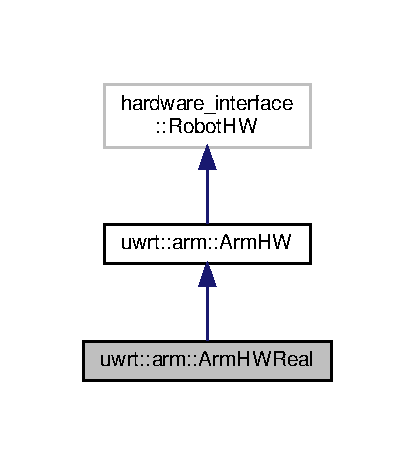
\includegraphics[width=199pt]{classuwrt_1_1arm_1_1_arm_h_w_real__inherit__graph}
\end{center}
\end{figure}


Collaboration diagram for uwrt\+:\+:arm\+:\+:Arm\+H\+W\+Real\+:
\nopagebreak
\begin{figure}[H]
\begin{center}
\leavevmode
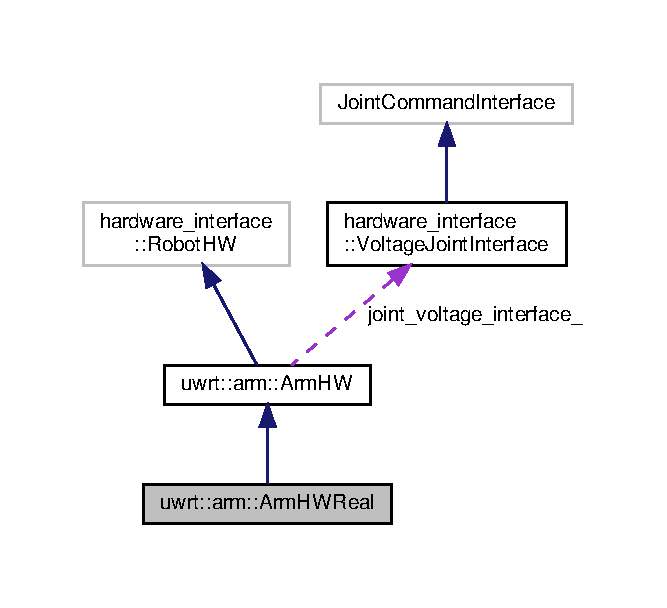
\includegraphics[width=320pt]{classuwrt_1_1arm_1_1_arm_h_w_real__coll__graph}
\end{center}
\end{figure}
\subsection*{Public Types}
\begin{DoxyCompactItemize}
\item 
enum \hyperlink{classuwrt_1_1arm_1_1_arm_h_w_real_ab0b3eb7330f9aa0f1101506fde2a889a}{Feedback\+Type} \{ \hyperlink{classuwrt_1_1arm_1_1_arm_h_w_real_ab0b3eb7330f9aa0f1101506fde2a889aa64a4abb154db9a6878c1d2e6053bd852}{G\+E\+N\+E\+R\+AL}, 
\hyperlink{classuwrt_1_1arm_1_1_arm_h_w_real_ab0b3eb7330f9aa0f1101506fde2a889aaded4c5ee9a1b43522d0a529e952bc21b}{P\+O\+S\+V\+EL}
 \}\begin{DoxyCompactList}\small\item\em Enum to distinguish between the type of feedback received over the C\+AN interface. \end{DoxyCompactList}
\end{DoxyCompactItemize}
\subsection*{Public Member Functions}
\begin{DoxyCompactItemize}
\item 
\hyperlink{classuwrt_1_1arm_1_1_arm_h_w_real_ad7edcfcf86fd221726402cbbf0f7a6d3}{Arm\+H\+W\+Real} (const std\+::string \&urdf\+\_\+str)
\begin{DoxyCompactList}\small\item\em Constructor. \end{DoxyCompactList}\item 
\hyperlink{classuwrt_1_1arm_1_1_arm_h_w_real_aa79a19f491094474cb91e6a07eecf0ee}{Arm\+H\+W\+Real} (const std\+::string \&name, const std\+::string \&urdf\+\_\+str)
\begin{DoxyCompactList}\small\item\em \+: Constructor \end{DoxyCompactList}\item 
virtual bool \hyperlink{classuwrt_1_1arm_1_1_arm_h_w_real_ab2556fef8e4666cb970113130e21a690}{init} (ros\+::\+Node\+Handle \&nh, ros\+::\+Node\+Handle \&arm\+\_\+hw\+\_\+nh)
\begin{DoxyCompactList}\small\item\em Initializes the hardware interface by registering all joints and interfaces. \end{DoxyCompactList}\item 
virtual void \hyperlink{classuwrt_1_1arm_1_1_arm_h_w_real_a7a4704f71c0652269a2e9c10907ca8b1}{read} (const ros\+::\+Time \&time, const ros\+::\+Duration \&period)
\begin{DoxyCompactList}\small\item\em Reads data from the arm. \end{DoxyCompactList}\item 
virtual void \hyperlink{classuwrt_1_1arm_1_1_arm_h_w_real_a25ab702964a8b1db7ea58b040189b820}{write} (const ros\+::\+Time \&time, const ros\+::\+Duration \&period)
\begin{DoxyCompactList}\small\item\em Writes data to the arm. \end{DoxyCompactList}\item 
void \hyperlink{classuwrt_1_1arm_1_1_arm_h_w_real_a5bc11742cda0b7826e45a12217c89965}{do\+Switch} (const std\+::list$<$ hardware\+\_\+interface\+::\+Controller\+Info $>$ \&start\+\_\+list, const std\+::list$<$ hardware\+\_\+interface\+::\+Controller\+Info $>$ \&stop\+\_\+list) override
\begin{DoxyCompactList}\small\item\em Starts/\+Stops controllers based on controller manager service calls. \end{DoxyCompactList}\end{DoxyCompactItemize}
\subsection*{Additional Inherited Members}


\subsection{Detailed Description}
Hardware Interface for the real Arm 

\subsection{Member Enumeration Documentation}
\mbox{\Hypertarget{classuwrt_1_1arm_1_1_arm_h_w_real_ab0b3eb7330f9aa0f1101506fde2a889a}\label{classuwrt_1_1arm_1_1_arm_h_w_real_ab0b3eb7330f9aa0f1101506fde2a889a}} 
\index{uwrt\+::arm\+::\+Arm\+H\+W\+Real@{uwrt\+::arm\+::\+Arm\+H\+W\+Real}!Feedback\+Type@{Feedback\+Type}}
\index{Feedback\+Type@{Feedback\+Type}!uwrt\+::arm\+::\+Arm\+H\+W\+Real@{uwrt\+::arm\+::\+Arm\+H\+W\+Real}}
\subsubsection{\texorpdfstring{Feedback\+Type}{FeedbackType}}
{\footnotesize\ttfamily enum \hyperlink{classuwrt_1_1arm_1_1_arm_h_w_real_ab0b3eb7330f9aa0f1101506fde2a889a}{uwrt\+::arm\+::\+Arm\+H\+W\+Real\+::\+Feedback\+Type}}



Enum to distinguish between the type of feedback received over the C\+AN interface. 

\begin{DoxyEnumFields}{Enumerator}
\raisebox{\heightof{T}}[0pt][0pt]{\index{G\+E\+N\+E\+R\+AL@{G\+E\+N\+E\+R\+AL}!uwrt\+::arm\+::\+Arm\+H\+W\+Real@{uwrt\+::arm\+::\+Arm\+H\+W\+Real}}\index{uwrt\+::arm\+::\+Arm\+H\+W\+Real@{uwrt\+::arm\+::\+Arm\+H\+W\+Real}!G\+E\+N\+E\+R\+AL@{G\+E\+N\+E\+R\+AL}}}\mbox{\Hypertarget{classuwrt_1_1arm_1_1_arm_h_w_real_ab0b3eb7330f9aa0f1101506fde2a889aa64a4abb154db9a6878c1d2e6053bd852}\label{classuwrt_1_1arm_1_1_arm_h_w_real_ab0b3eb7330f9aa0f1101506fde2a889aa64a4abb154db9a6878c1d2e6053bd852}} 
G\+E\+N\+E\+R\+AL&\\
\hline

\raisebox{\heightof{T}}[0pt][0pt]{\index{P\+O\+S\+V\+EL@{P\+O\+S\+V\+EL}!uwrt\+::arm\+::\+Arm\+H\+W\+Real@{uwrt\+::arm\+::\+Arm\+H\+W\+Real}}\index{uwrt\+::arm\+::\+Arm\+H\+W\+Real@{uwrt\+::arm\+::\+Arm\+H\+W\+Real}!P\+O\+S\+V\+EL@{P\+O\+S\+V\+EL}}}\mbox{\Hypertarget{classuwrt_1_1arm_1_1_arm_h_w_real_ab0b3eb7330f9aa0f1101506fde2a889aaded4c5ee9a1b43522d0a529e952bc21b}\label{classuwrt_1_1arm_1_1_arm_h_w_real_ab0b3eb7330f9aa0f1101506fde2a889aaded4c5ee9a1b43522d0a529e952bc21b}} 
P\+O\+S\+V\+EL&\\
\hline

\end{DoxyEnumFields}


\subsection{Constructor \& Destructor Documentation}
\mbox{\Hypertarget{classuwrt_1_1arm_1_1_arm_h_w_real_ad7edcfcf86fd221726402cbbf0f7a6d3}\label{classuwrt_1_1arm_1_1_arm_h_w_real_ad7edcfcf86fd221726402cbbf0f7a6d3}} 
\index{uwrt\+::arm\+::\+Arm\+H\+W\+Real@{uwrt\+::arm\+::\+Arm\+H\+W\+Real}!Arm\+H\+W\+Real@{Arm\+H\+W\+Real}}
\index{Arm\+H\+W\+Real@{Arm\+H\+W\+Real}!uwrt\+::arm\+::\+Arm\+H\+W\+Real@{uwrt\+::arm\+::\+Arm\+H\+W\+Real}}
\subsubsection{\texorpdfstring{Arm\+H\+W\+Real()}{ArmHWReal()}\hspace{0.1cm}{\footnotesize\ttfamily [1/2]}}
{\footnotesize\ttfamily uwrt\+::arm\+::\+Arm\+H\+W\+Real\+::\+Arm\+H\+W\+Real (\begin{DoxyParamCaption}\item[{const std\+::string \&}]{urdf\+\_\+str }\end{DoxyParamCaption})\hspace{0.3cm}{\ttfamily [explicit]}}



Constructor. 


\begin{DoxyParams}{Parameters}
{\em urdf\+\_\+str} & U\+R\+DF of the arm in string format \\
\hline
\end{DoxyParams}
\mbox{\Hypertarget{classuwrt_1_1arm_1_1_arm_h_w_real_aa79a19f491094474cb91e6a07eecf0ee}\label{classuwrt_1_1arm_1_1_arm_h_w_real_aa79a19f491094474cb91e6a07eecf0ee}} 
\index{uwrt\+::arm\+::\+Arm\+H\+W\+Real@{uwrt\+::arm\+::\+Arm\+H\+W\+Real}!Arm\+H\+W\+Real@{Arm\+H\+W\+Real}}
\index{Arm\+H\+W\+Real@{Arm\+H\+W\+Real}!uwrt\+::arm\+::\+Arm\+H\+W\+Real@{uwrt\+::arm\+::\+Arm\+H\+W\+Real}}
\subsubsection{\texorpdfstring{Arm\+H\+W\+Real()}{ArmHWReal()}\hspace{0.1cm}{\footnotesize\ttfamily [2/2]}}
{\footnotesize\ttfamily uwrt\+::arm\+::\+Arm\+H\+W\+Real\+::\+Arm\+H\+W\+Real (\begin{DoxyParamCaption}\item[{const std\+::string \&}]{name,  }\item[{const std\+::string \&}]{urdf\+\_\+str }\end{DoxyParamCaption})}



\+: Constructor 


\begin{DoxyParams}{Parameters}
{\em name} & Arbitrary name for an instance of this class \\
\hline
{\em urdf\+\_\+str} & U\+R\+DF of the arm in string format \\
\hline
\end{DoxyParams}


\subsection{Member Function Documentation}
\mbox{\Hypertarget{classuwrt_1_1arm_1_1_arm_h_w_real_a5bc11742cda0b7826e45a12217c89965}\label{classuwrt_1_1arm_1_1_arm_h_w_real_a5bc11742cda0b7826e45a12217c89965}} 
\index{uwrt\+::arm\+::\+Arm\+H\+W\+Real@{uwrt\+::arm\+::\+Arm\+H\+W\+Real}!do\+Switch@{do\+Switch}}
\index{do\+Switch@{do\+Switch}!uwrt\+::arm\+::\+Arm\+H\+W\+Real@{uwrt\+::arm\+::\+Arm\+H\+W\+Real}}
\subsubsection{\texorpdfstring{do\+Switch()}{doSwitch()}}
{\footnotesize\ttfamily void uwrt\+::arm\+::\+Arm\+H\+W\+Real\+::do\+Switch (\begin{DoxyParamCaption}\item[{const std\+::list$<$ hardware\+\_\+interface\+::\+Controller\+Info $>$ \&}]{start\+\_\+list,  }\item[{const std\+::list$<$ hardware\+\_\+interface\+::\+Controller\+Info $>$ \&}]{stop\+\_\+list }\end{DoxyParamCaption})\hspace{0.3cm}{\ttfamily [override]}}



Starts/\+Stops controllers based on controller manager service calls. 


\begin{DoxyParams}{Parameters}
{\em start\+\_\+list} & Controllers to start \\
\hline
{\em stop\+\_\+list} & Controllers to stop \\
\hline
\end{DoxyParams}
\mbox{\Hypertarget{classuwrt_1_1arm_1_1_arm_h_w_real_ab2556fef8e4666cb970113130e21a690}\label{classuwrt_1_1arm_1_1_arm_h_w_real_ab2556fef8e4666cb970113130e21a690}} 
\index{uwrt\+::arm\+::\+Arm\+H\+W\+Real@{uwrt\+::arm\+::\+Arm\+H\+W\+Real}!init@{init}}
\index{init@{init}!uwrt\+::arm\+::\+Arm\+H\+W\+Real@{uwrt\+::arm\+::\+Arm\+H\+W\+Real}}
\subsubsection{\texorpdfstring{init()}{init()}}
{\footnotesize\ttfamily bool uwrt\+::arm\+::\+Arm\+H\+W\+Real\+::init (\begin{DoxyParamCaption}\item[{ros\+::\+Node\+Handle \&}]{nh,  }\item[{ros\+::\+Node\+Handle \&}]{arm\+\_\+hw\+\_\+nh }\end{DoxyParamCaption})\hspace{0.3cm}{\ttfamily [virtual]}}



Initializes the hardware interface by registering all joints and interfaces. 


\begin{DoxyParams}{Parameters}
{\em nh} & Nodehandle for the root of the arm namespace \\
\hline
{\em arm\+\_\+hw\+\_\+nh} & Nodehandle in the namespace of the arm hardware interface \\
\hline
\end{DoxyParams}
\mbox{\Hypertarget{classuwrt_1_1arm_1_1_arm_h_w_real_a7a4704f71c0652269a2e9c10907ca8b1}\label{classuwrt_1_1arm_1_1_arm_h_w_real_a7a4704f71c0652269a2e9c10907ca8b1}} 
\index{uwrt\+::arm\+::\+Arm\+H\+W\+Real@{uwrt\+::arm\+::\+Arm\+H\+W\+Real}!read@{read}}
\index{read@{read}!uwrt\+::arm\+::\+Arm\+H\+W\+Real@{uwrt\+::arm\+::\+Arm\+H\+W\+Real}}
\subsubsection{\texorpdfstring{read()}{read()}}
{\footnotesize\ttfamily void uwrt\+::arm\+::\+Arm\+H\+W\+Real\+::read (\begin{DoxyParamCaption}\item[{const ros\+::\+Time \&}]{time,  }\item[{const ros\+::\+Duration \&}]{period }\end{DoxyParamCaption})\hspace{0.3cm}{\ttfamily [virtual]}}



Reads data from the arm. 


\begin{DoxyParams}{Parameters}
{\em time} & The current time \\
\hline
{\em period} & The time passes since last call to read \\
\hline
\end{DoxyParams}


Implements \hyperlink{classuwrt_1_1arm_1_1_arm_h_w_af2164103badfa99373f787b8a3cecb6b}{uwrt\+::arm\+::\+Arm\+HW}.

\mbox{\Hypertarget{classuwrt_1_1arm_1_1_arm_h_w_real_a25ab702964a8b1db7ea58b040189b820}\label{classuwrt_1_1arm_1_1_arm_h_w_real_a25ab702964a8b1db7ea58b040189b820}} 
\index{uwrt\+::arm\+::\+Arm\+H\+W\+Real@{uwrt\+::arm\+::\+Arm\+H\+W\+Real}!write@{write}}
\index{write@{write}!uwrt\+::arm\+::\+Arm\+H\+W\+Real@{uwrt\+::arm\+::\+Arm\+H\+W\+Real}}
\subsubsection{\texorpdfstring{write()}{write()}}
{\footnotesize\ttfamily void uwrt\+::arm\+::\+Arm\+H\+W\+Real\+::write (\begin{DoxyParamCaption}\item[{const ros\+::\+Time \&}]{time,  }\item[{const ros\+::\+Duration \&}]{period }\end{DoxyParamCaption})\hspace{0.3cm}{\ttfamily [virtual]}}



Writes data to the arm. 


\begin{DoxyParams}{Parameters}
{\em time} & The current time \\
\hline
{\em period} & The time passes since last call to write \\
\hline
\end{DoxyParams}


Implements \hyperlink{classuwrt_1_1arm_1_1_arm_h_w_a934119487836109e24d9054f10e9832f}{uwrt\+::arm\+::\+Arm\+HW}.



The documentation for this class was generated from the following files\+:\begin{DoxyCompactItemize}
\item 
uwrt\+\_\+arm\+\_\+hw/include/uwrt\+\_\+arm\+\_\+hw/\hyperlink{arm__hw__real_8h}{arm\+\_\+hw\+\_\+real.\+h}\item 
uwrt\+\_\+arm\+\_\+hw/src/\hyperlink{arm__hw__real_8cpp}{arm\+\_\+hw\+\_\+real.\+cpp}\end{DoxyCompactItemize}

\hypertarget{classuwrt_1_1arm_1_1_arm_h_w_sim}{}\section{uwrt\+:\+:arm\+:\+:Arm\+H\+W\+Sim Class Reference}
\label{classuwrt_1_1arm_1_1_arm_h_w_sim}\index{uwrt\+::arm\+::\+Arm\+H\+W\+Sim@{uwrt\+::arm\+::\+Arm\+H\+W\+Sim}}


{\ttfamily \#include $<$arm\+\_\+hw\+\_\+sim.\+h$>$}



Inheritance diagram for uwrt\+:\+:arm\+:\+:Arm\+H\+W\+Sim\+:
\nopagebreak
\begin{figure}[H]
\begin{center}
\leavevmode
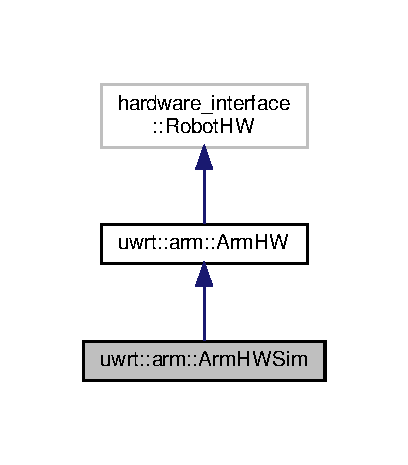
\includegraphics[width=196pt]{classuwrt_1_1arm_1_1_arm_h_w_sim__inherit__graph}
\end{center}
\end{figure}


Collaboration diagram for uwrt\+:\+:arm\+:\+:Arm\+H\+W\+Sim\+:
\nopagebreak
\begin{figure}[H]
\begin{center}
\leavevmode
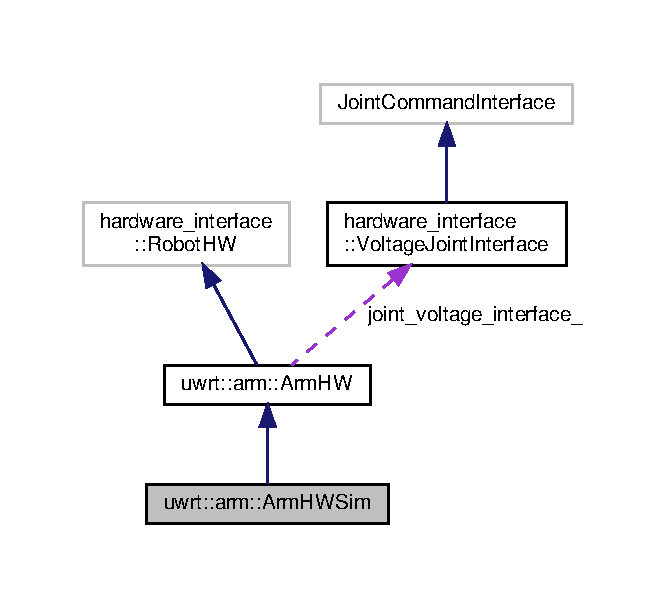
\includegraphics[width=320pt]{classuwrt_1_1arm_1_1_arm_h_w_sim__coll__graph}
\end{center}
\end{figure}
\subsection*{Public Member Functions}
\begin{DoxyCompactItemize}
\item 
\hyperlink{classuwrt_1_1arm_1_1_arm_h_w_sim_aaa787422131f1db3f639e5905545a839}{Arm\+H\+W\+Sim} (gazebo\+::physics\+::\+Model\+Ptr model, const std\+::string \&urdf\+\_\+str)
\begin{DoxyCompactList}\small\item\em Constructor. \end{DoxyCompactList}\item 
\hyperlink{classuwrt_1_1arm_1_1_arm_h_w_sim_ac0764d307f3b885dccc49c36545dfcd3}{Arm\+H\+W\+Sim} (const std\+::string \&name, gazebo\+::physics\+::\+Model\+Ptr model, const std\+::string \&urdf\+\_\+str)
\begin{DoxyCompactList}\small\item\em Constructor. \end{DoxyCompactList}\item 
virtual bool \hyperlink{classuwrt_1_1arm_1_1_arm_h_w_sim_ab099f7bf8a4a9b27d8699f61c71ad30e}{init} (ros\+::\+Node\+Handle \&nh, ros\+::\+Node\+Handle \&arm\+\_\+hw\+\_\+nh)
\begin{DoxyCompactList}\small\item\em Initializes the hardware interface by registering all joints and interfaces. \end{DoxyCompactList}\item 
virtual void \hyperlink{classuwrt_1_1arm_1_1_arm_h_w_sim_a78eb2303fba768155763a25797c0eecf}{read} (const ros\+::\+Time \&time, const ros\+::\+Duration \&period)
\begin{DoxyCompactList}\small\item\em Reads data from the arm. \end{DoxyCompactList}\item 
virtual void \hyperlink{classuwrt_1_1arm_1_1_arm_h_w_sim_aa334fca03f76265ca8ec2da3be53991f}{write} (const ros\+::\+Time \&time, const ros\+::\+Duration \&period)
\begin{DoxyCompactList}\small\item\em Writes data to the arm. \end{DoxyCompactList}\end{DoxyCompactItemize}
\subsection*{Additional Inherited Members}


\subsection{Detailed Description}
Hardware Interface for Gazebo simulation of the Arm 

\subsection{Constructor \& Destructor Documentation}
\mbox{\Hypertarget{classuwrt_1_1arm_1_1_arm_h_w_sim_aaa787422131f1db3f639e5905545a839}\label{classuwrt_1_1arm_1_1_arm_h_w_sim_aaa787422131f1db3f639e5905545a839}} 
\index{uwrt\+::arm\+::\+Arm\+H\+W\+Sim@{uwrt\+::arm\+::\+Arm\+H\+W\+Sim}!Arm\+H\+W\+Sim@{Arm\+H\+W\+Sim}}
\index{Arm\+H\+W\+Sim@{Arm\+H\+W\+Sim}!uwrt\+::arm\+::\+Arm\+H\+W\+Sim@{uwrt\+::arm\+::\+Arm\+H\+W\+Sim}}
\subsubsection{\texorpdfstring{Arm\+H\+W\+Sim()}{ArmHWSim()}\hspace{0.1cm}{\footnotesize\ttfamily [1/2]}}
{\footnotesize\ttfamily uwrt\+::arm\+::\+Arm\+H\+W\+Sim\+::\+Arm\+H\+W\+Sim (\begin{DoxyParamCaption}\item[{gazebo\+::physics\+::\+Model\+Ptr}]{model,  }\item[{const std\+::string \&}]{urdf\+\_\+str }\end{DoxyParamCaption})}



Constructor. 


\begin{DoxyParams}{Parameters}
{\em model} & Pointer to the simulated arm object in gazebo \\
\hline
{\em urdf\+\_\+str} & U\+R\+DF of the Arm in string format \\
\hline
\end{DoxyParams}
\mbox{\Hypertarget{classuwrt_1_1arm_1_1_arm_h_w_sim_ac0764d307f3b885dccc49c36545dfcd3}\label{classuwrt_1_1arm_1_1_arm_h_w_sim_ac0764d307f3b885dccc49c36545dfcd3}} 
\index{uwrt\+::arm\+::\+Arm\+H\+W\+Sim@{uwrt\+::arm\+::\+Arm\+H\+W\+Sim}!Arm\+H\+W\+Sim@{Arm\+H\+W\+Sim}}
\index{Arm\+H\+W\+Sim@{Arm\+H\+W\+Sim}!uwrt\+::arm\+::\+Arm\+H\+W\+Sim@{uwrt\+::arm\+::\+Arm\+H\+W\+Sim}}
\subsubsection{\texorpdfstring{Arm\+H\+W\+Sim()}{ArmHWSim()}\hspace{0.1cm}{\footnotesize\ttfamily [2/2]}}
{\footnotesize\ttfamily uwrt\+::arm\+::\+Arm\+H\+W\+Sim\+::\+Arm\+H\+W\+Sim (\begin{DoxyParamCaption}\item[{const std\+::string \&}]{name,  }\item[{gazebo\+::physics\+::\+Model\+Ptr}]{model,  }\item[{const std\+::string \&}]{urdf\+\_\+str }\end{DoxyParamCaption})}



Constructor. 


\begin{DoxyParams}{Parameters}
{\em name} & Arbitrary name for an instance of this class \\
\hline
{\em model} & Pointer to the simulated arm object in gazebo \\
\hline
{\em urdf\+\_\+str} & U\+R\+DF of the Arm in string format \\
\hline
\end{DoxyParams}


\subsection{Member Function Documentation}
\mbox{\Hypertarget{classuwrt_1_1arm_1_1_arm_h_w_sim_ab099f7bf8a4a9b27d8699f61c71ad30e}\label{classuwrt_1_1arm_1_1_arm_h_w_sim_ab099f7bf8a4a9b27d8699f61c71ad30e}} 
\index{uwrt\+::arm\+::\+Arm\+H\+W\+Sim@{uwrt\+::arm\+::\+Arm\+H\+W\+Sim}!init@{init}}
\index{init@{init}!uwrt\+::arm\+::\+Arm\+H\+W\+Sim@{uwrt\+::arm\+::\+Arm\+H\+W\+Sim}}
\subsubsection{\texorpdfstring{init()}{init()}}
{\footnotesize\ttfamily bool uwrt\+::arm\+::\+Arm\+H\+W\+Sim\+::init (\begin{DoxyParamCaption}\item[{ros\+::\+Node\+Handle \&}]{nh,  }\item[{ros\+::\+Node\+Handle \&}]{arm\+\_\+hw\+\_\+nh }\end{DoxyParamCaption})\hspace{0.3cm}{\ttfamily [virtual]}}



Initializes the hardware interface by registering all joints and interfaces. 


\begin{DoxyParams}{Parameters}
{\em nh} & Nodehandle for the root of the arm namespace \\
\hline
{\em arm\+\_\+hw\+\_\+nh} & Nodehandle in the namespace of the arm hardware interface \\
\hline
\end{DoxyParams}
\mbox{\Hypertarget{classuwrt_1_1arm_1_1_arm_h_w_sim_a78eb2303fba768155763a25797c0eecf}\label{classuwrt_1_1arm_1_1_arm_h_w_sim_a78eb2303fba768155763a25797c0eecf}} 
\index{uwrt\+::arm\+::\+Arm\+H\+W\+Sim@{uwrt\+::arm\+::\+Arm\+H\+W\+Sim}!read@{read}}
\index{read@{read}!uwrt\+::arm\+::\+Arm\+H\+W\+Sim@{uwrt\+::arm\+::\+Arm\+H\+W\+Sim}}
\subsubsection{\texorpdfstring{read()}{read()}}
{\footnotesize\ttfamily void uwrt\+::arm\+::\+Arm\+H\+W\+Sim\+::read (\begin{DoxyParamCaption}\item[{const ros\+::\+Time \&}]{time,  }\item[{const ros\+::\+Duration \&}]{period }\end{DoxyParamCaption})\hspace{0.3cm}{\ttfamily [virtual]}}



Reads data from the arm. 


\begin{DoxyParams}{Parameters}
{\em time} & The current time \\
\hline
{\em period} & The time passes since last call to read \\
\hline
\end{DoxyParams}


Implements \hyperlink{classuwrt_1_1arm_1_1_arm_h_w_af2164103badfa99373f787b8a3cecb6b}{uwrt\+::arm\+::\+Arm\+HW}.

\mbox{\Hypertarget{classuwrt_1_1arm_1_1_arm_h_w_sim_aa334fca03f76265ca8ec2da3be53991f}\label{classuwrt_1_1arm_1_1_arm_h_w_sim_aa334fca03f76265ca8ec2da3be53991f}} 
\index{uwrt\+::arm\+::\+Arm\+H\+W\+Sim@{uwrt\+::arm\+::\+Arm\+H\+W\+Sim}!write@{write}}
\index{write@{write}!uwrt\+::arm\+::\+Arm\+H\+W\+Sim@{uwrt\+::arm\+::\+Arm\+H\+W\+Sim}}
\subsubsection{\texorpdfstring{write()}{write()}}
{\footnotesize\ttfamily void uwrt\+::arm\+::\+Arm\+H\+W\+Sim\+::write (\begin{DoxyParamCaption}\item[{const ros\+::\+Time \&}]{time,  }\item[{const ros\+::\+Duration \&}]{period }\end{DoxyParamCaption})\hspace{0.3cm}{\ttfamily [virtual]}}



Writes data to the arm. 


\begin{DoxyParams}{Parameters}
{\em time} & The current time \\
\hline
{\em period} & The time passes since last call to write \\
\hline
\end{DoxyParams}


Implements \hyperlink{classuwrt_1_1arm_1_1_arm_h_w_a934119487836109e24d9054f10e9832f}{uwrt\+::arm\+::\+Arm\+HW}.



The documentation for this class was generated from the following files\+:\begin{DoxyCompactItemize}
\item 
uwrt\+\_\+arm\+\_\+hw/include/uwrt\+\_\+arm\+\_\+hw/\hyperlink{arm__hw__sim_8h}{arm\+\_\+hw\+\_\+sim.\+h}\item 
uwrt\+\_\+arm\+\_\+hw/src/\hyperlink{arm__hw__sim_8cpp}{arm\+\_\+hw\+\_\+sim.\+cpp}\end{DoxyCompactItemize}

\hypertarget{structuwrt_1_1arm_1_1can__id_1_1_calibrate}{}\section{uwrt\+:\+:arm\+:\+:can\+\_\+id\+:\+:Calibrate Struct Reference}
\label{structuwrt_1_1arm_1_1can__id_1_1_calibrate}\index{uwrt\+::arm\+::can\+\_\+id\+::\+Calibrate@{uwrt\+::arm\+::can\+\_\+id\+::\+Calibrate}}


{\ttfamily \#include $<$can\+\_\+config.\+h$>$}

\subsection*{Static Public Attributes}
\begin{DoxyCompactItemize}
\item 
static const canid\+\_\+t \hyperlink{structuwrt_1_1arm_1_1can__id_1_1_calibrate_a61674e5392384ebd496a6bdff1b3e383}{W\+R\+I\+ST} = 0x74C
\item 
static const canid\+\_\+t \hyperlink{structuwrt_1_1arm_1_1can__id_1_1_calibrate_a24b0f9e55fcf76450ee9f28e51e6719e}{C\+L\+AW} = 0x74D
\end{DoxyCompactItemize}


\subsection{Detailed Description}
C\+AN I\+Ds for calibration procedures 

\subsection{Member Data Documentation}
\mbox{\Hypertarget{structuwrt_1_1arm_1_1can__id_1_1_calibrate_a24b0f9e55fcf76450ee9f28e51e6719e}\label{structuwrt_1_1arm_1_1can__id_1_1_calibrate_a24b0f9e55fcf76450ee9f28e51e6719e}} 
\index{uwrt\+::arm\+::can\+\_\+id\+::\+Calibrate@{uwrt\+::arm\+::can\+\_\+id\+::\+Calibrate}!C\+L\+AW@{C\+L\+AW}}
\index{C\+L\+AW@{C\+L\+AW}!uwrt\+::arm\+::can\+\_\+id\+::\+Calibrate@{uwrt\+::arm\+::can\+\_\+id\+::\+Calibrate}}
\subsubsection{\texorpdfstring{C\+L\+AW}{CLAW}}
{\footnotesize\ttfamily const canid\+\_\+t uwrt\+::arm\+::can\+\_\+id\+::\+Calibrate\+::\+C\+L\+AW = 0x74D\hspace{0.3cm}{\ttfamily [static]}}

\mbox{\Hypertarget{structuwrt_1_1arm_1_1can__id_1_1_calibrate_a61674e5392384ebd496a6bdff1b3e383}\label{structuwrt_1_1arm_1_1can__id_1_1_calibrate_a61674e5392384ebd496a6bdff1b3e383}} 
\index{uwrt\+::arm\+::can\+\_\+id\+::\+Calibrate@{uwrt\+::arm\+::can\+\_\+id\+::\+Calibrate}!W\+R\+I\+ST@{W\+R\+I\+ST}}
\index{W\+R\+I\+ST@{W\+R\+I\+ST}!uwrt\+::arm\+::can\+\_\+id\+::\+Calibrate@{uwrt\+::arm\+::can\+\_\+id\+::\+Calibrate}}
\subsubsection{\texorpdfstring{W\+R\+I\+ST}{WRIST}}
{\footnotesize\ttfamily const canid\+\_\+t uwrt\+::arm\+::can\+\_\+id\+::\+Calibrate\+::\+W\+R\+I\+ST = 0x74C\hspace{0.3cm}{\ttfamily [static]}}



The documentation for this struct was generated from the following file\+:\begin{DoxyCompactItemize}
\item 
uwrt\+\_\+arm\+\_\+hw/include/uwrt\+\_\+arm\+\_\+hw/\hyperlink{can__config_8h}{can\+\_\+config.\+h}\end{DoxyCompactItemize}

\hypertarget{classuwrt_1_1arm_1_1_delta_joint_publisher}{}\section{uwrt\+:\+:arm\+:\+:Delta\+Joint\+Publisher Class Reference}
\label{classuwrt_1_1arm_1_1_delta_joint_publisher}\index{uwrt\+::arm\+::\+Delta\+Joint\+Publisher@{uwrt\+::arm\+::\+Delta\+Joint\+Publisher}}


{\ttfamily \#include $<$delta\+\_\+joint\+\_\+publisher.\+h$>$}

\subsection*{Public Member Functions}
\begin{DoxyCompactItemize}
\item 
\hyperlink{classuwrt_1_1arm_1_1_delta_joint_publisher_a2a28037514970085647a7a83f8e41cba}{Delta\+Joint\+Publisher} (ros\+::\+Node\+Handle \&nh, ros\+::\+Node\+Handle \&priv\+\_\+nh)
\item 
\hyperlink{classuwrt_1_1arm_1_1_delta_joint_publisher_a15ad0c41ea3aa86372ed7e7f3d32d499}{$\sim$\+Delta\+Joint\+Publisher} ()
\item 
void \hyperlink{classuwrt_1_1arm_1_1_delta_joint_publisher_ae552d731968245c249fe30596ea7d1f1}{spin} ()
\end{DoxyCompactItemize}
\subsection*{Protected Member Functions}
\begin{DoxyCompactItemize}
\item 
void \hyperlink{classuwrt_1_1arm_1_1_delta_joint_publisher_abc33c0374665b4b0f630a220eb13d3b5}{arm\+Command\+Callback} (const uwrt\+\_\+arm\+\_\+msgs\+::\+U\+W\+R\+T\+Arm\+Command\+Const\+Ptr \&arm\+\_\+command)
\item 
void \hyperlink{classuwrt_1_1arm_1_1_delta_joint_publisher_a45e0f2e8e7cfdb8dc6794e63844c035a}{arm\+Command\+To\+Joint\+Jog} (const uwrt\+\_\+arm\+\_\+msgs\+::\+U\+W\+R\+T\+Arm\+Command \&arm\+\_\+command, control\+\_\+msgs\+::\+Joint\+Jog \&jog\+\_\+command)
\end{DoxyCompactItemize}
\subsection*{Protected Attributes}
\begin{DoxyCompactItemize}
\item 
ros\+::\+Node\+Handle \hyperlink{classuwrt_1_1arm_1_1_delta_joint_publisher_a6b8d05a3b56e026880a6db5eacfffcde}{nh\+\_\+}
\item 
ros\+::\+Node\+Handle \hyperlink{classuwrt_1_1arm_1_1_delta_joint_publisher_ab9cb80c9bd9410d122a19730123c3e00}{priv\+\_\+nh\+\_\+}
\end{DoxyCompactItemize}


\subsection{Constructor \& Destructor Documentation}
\mbox{\Hypertarget{classuwrt_1_1arm_1_1_delta_joint_publisher_a2a28037514970085647a7a83f8e41cba}\label{classuwrt_1_1arm_1_1_delta_joint_publisher_a2a28037514970085647a7a83f8e41cba}} 
\index{uwrt\+::arm\+::\+Delta\+Joint\+Publisher@{uwrt\+::arm\+::\+Delta\+Joint\+Publisher}!Delta\+Joint\+Publisher@{Delta\+Joint\+Publisher}}
\index{Delta\+Joint\+Publisher@{Delta\+Joint\+Publisher}!uwrt\+::arm\+::\+Delta\+Joint\+Publisher@{uwrt\+::arm\+::\+Delta\+Joint\+Publisher}}
\subsubsection{\texorpdfstring{Delta\+Joint\+Publisher()}{DeltaJointPublisher()}}
{\footnotesize\ttfamily uwrt\+::arm\+::\+Delta\+Joint\+Publisher\+::\+Delta\+Joint\+Publisher (\begin{DoxyParamCaption}\item[{ros\+::\+Node\+Handle \&}]{nh,  }\item[{ros\+::\+Node\+Handle \&}]{priv\+\_\+nh }\end{DoxyParamCaption})}

\mbox{\Hypertarget{classuwrt_1_1arm_1_1_delta_joint_publisher_a15ad0c41ea3aa86372ed7e7f3d32d499}\label{classuwrt_1_1arm_1_1_delta_joint_publisher_a15ad0c41ea3aa86372ed7e7f3d32d499}} 
\index{uwrt\+::arm\+::\+Delta\+Joint\+Publisher@{uwrt\+::arm\+::\+Delta\+Joint\+Publisher}!````~Delta\+Joint\+Publisher@{$\sim$\+Delta\+Joint\+Publisher}}
\index{````~Delta\+Joint\+Publisher@{$\sim$\+Delta\+Joint\+Publisher}!uwrt\+::arm\+::\+Delta\+Joint\+Publisher@{uwrt\+::arm\+::\+Delta\+Joint\+Publisher}}
\subsubsection{\texorpdfstring{$\sim$\+Delta\+Joint\+Publisher()}{~DeltaJointPublisher()}}
{\footnotesize\ttfamily uwrt\+::arm\+::\+Delta\+Joint\+Publisher\+::$\sim$\+Delta\+Joint\+Publisher (\begin{DoxyParamCaption}{ }\end{DoxyParamCaption})}



\subsection{Member Function Documentation}
\mbox{\Hypertarget{classuwrt_1_1arm_1_1_delta_joint_publisher_abc33c0374665b4b0f630a220eb13d3b5}\label{classuwrt_1_1arm_1_1_delta_joint_publisher_abc33c0374665b4b0f630a220eb13d3b5}} 
\index{uwrt\+::arm\+::\+Delta\+Joint\+Publisher@{uwrt\+::arm\+::\+Delta\+Joint\+Publisher}!arm\+Command\+Callback@{arm\+Command\+Callback}}
\index{arm\+Command\+Callback@{arm\+Command\+Callback}!uwrt\+::arm\+::\+Delta\+Joint\+Publisher@{uwrt\+::arm\+::\+Delta\+Joint\+Publisher}}
\subsubsection{\texorpdfstring{arm\+Command\+Callback()}{armCommandCallback()}}
{\footnotesize\ttfamily void uwrt\+::arm\+::\+Delta\+Joint\+Publisher\+::arm\+Command\+Callback (\begin{DoxyParamCaption}\item[{const uwrt\+\_\+arm\+\_\+msgs\+::\+U\+W\+R\+T\+Arm\+Command\+Const\+Ptr \&}]{arm\+\_\+command }\end{DoxyParamCaption})\hspace{0.3cm}{\ttfamily [protected]}}

\mbox{\Hypertarget{classuwrt_1_1arm_1_1_delta_joint_publisher_a45e0f2e8e7cfdb8dc6794e63844c035a}\label{classuwrt_1_1arm_1_1_delta_joint_publisher_a45e0f2e8e7cfdb8dc6794e63844c035a}} 
\index{uwrt\+::arm\+::\+Delta\+Joint\+Publisher@{uwrt\+::arm\+::\+Delta\+Joint\+Publisher}!arm\+Command\+To\+Joint\+Jog@{arm\+Command\+To\+Joint\+Jog}}
\index{arm\+Command\+To\+Joint\+Jog@{arm\+Command\+To\+Joint\+Jog}!uwrt\+::arm\+::\+Delta\+Joint\+Publisher@{uwrt\+::arm\+::\+Delta\+Joint\+Publisher}}
\subsubsection{\texorpdfstring{arm\+Command\+To\+Joint\+Jog()}{armCommandToJointJog()}}
{\footnotesize\ttfamily void uwrt\+::arm\+::\+Delta\+Joint\+Publisher\+::arm\+Command\+To\+Joint\+Jog (\begin{DoxyParamCaption}\item[{const uwrt\+\_\+arm\+\_\+msgs\+::\+U\+W\+R\+T\+Arm\+Command \&}]{arm\+\_\+command,  }\item[{control\+\_\+msgs\+::\+Joint\+Jog \&}]{jog\+\_\+command }\end{DoxyParamCaption})\hspace{0.3cm}{\ttfamily [protected]}}

\mbox{\Hypertarget{classuwrt_1_1arm_1_1_delta_joint_publisher_ae552d731968245c249fe30596ea7d1f1}\label{classuwrt_1_1arm_1_1_delta_joint_publisher_ae552d731968245c249fe30596ea7d1f1}} 
\index{uwrt\+::arm\+::\+Delta\+Joint\+Publisher@{uwrt\+::arm\+::\+Delta\+Joint\+Publisher}!spin@{spin}}
\index{spin@{spin}!uwrt\+::arm\+::\+Delta\+Joint\+Publisher@{uwrt\+::arm\+::\+Delta\+Joint\+Publisher}}
\subsubsection{\texorpdfstring{spin()}{spin()}}
{\footnotesize\ttfamily void uwrt\+::arm\+::\+Delta\+Joint\+Publisher\+::spin (\begin{DoxyParamCaption}{ }\end{DoxyParamCaption})}



\subsection{Member Data Documentation}
\mbox{\Hypertarget{classuwrt_1_1arm_1_1_delta_joint_publisher_a6b8d05a3b56e026880a6db5eacfffcde}\label{classuwrt_1_1arm_1_1_delta_joint_publisher_a6b8d05a3b56e026880a6db5eacfffcde}} 
\index{uwrt\+::arm\+::\+Delta\+Joint\+Publisher@{uwrt\+::arm\+::\+Delta\+Joint\+Publisher}!nh\+\_\+@{nh\+\_\+}}
\index{nh\+\_\+@{nh\+\_\+}!uwrt\+::arm\+::\+Delta\+Joint\+Publisher@{uwrt\+::arm\+::\+Delta\+Joint\+Publisher}}
\subsubsection{\texorpdfstring{nh\+\_\+}{nh\_}}
{\footnotesize\ttfamily ros\+::\+Node\+Handle uwrt\+::arm\+::\+Delta\+Joint\+Publisher\+::nh\+\_\+\hspace{0.3cm}{\ttfamily [protected]}}

\mbox{\Hypertarget{classuwrt_1_1arm_1_1_delta_joint_publisher_ab9cb80c9bd9410d122a19730123c3e00}\label{classuwrt_1_1arm_1_1_delta_joint_publisher_ab9cb80c9bd9410d122a19730123c3e00}} 
\index{uwrt\+::arm\+::\+Delta\+Joint\+Publisher@{uwrt\+::arm\+::\+Delta\+Joint\+Publisher}!priv\+\_\+nh\+\_\+@{priv\+\_\+nh\+\_\+}}
\index{priv\+\_\+nh\+\_\+@{priv\+\_\+nh\+\_\+}!uwrt\+::arm\+::\+Delta\+Joint\+Publisher@{uwrt\+::arm\+::\+Delta\+Joint\+Publisher}}
\subsubsection{\texorpdfstring{priv\+\_\+nh\+\_\+}{priv\_nh\_}}
{\footnotesize\ttfamily ros\+::\+Node\+Handle uwrt\+::arm\+::\+Delta\+Joint\+Publisher\+::priv\+\_\+nh\+\_\+\hspace{0.3cm}{\ttfamily [protected]}}



The documentation for this class was generated from the following files\+:\begin{DoxyCompactItemize}
\item 
uwrt\+\_\+arm\+\_\+control/include/uwrt\+\_\+arm\+\_\+control/\hyperlink{delta__joint__publisher_8h}{delta\+\_\+joint\+\_\+publisher.\+h}\item 
uwrt\+\_\+arm\+\_\+control/src/\hyperlink{delta__joint__publisher_8cpp}{delta\+\_\+joint\+\_\+publisher.\+cpp}\end{DoxyCompactItemize}

\hypertarget{classuwrt_1_1arm_1_1_gazebo_arm_control_plugin}{}\section{uwrt\+:\+:arm\+:\+:Gazebo\+Arm\+Control\+Plugin Class Reference}
\label{classuwrt_1_1arm_1_1_gazebo_arm_control_plugin}\index{uwrt\+::arm\+::\+Gazebo\+Arm\+Control\+Plugin@{uwrt\+::arm\+::\+Gazebo\+Arm\+Control\+Plugin}}


{\ttfamily \#include $<$gazebo\+\_\+arm\+\_\+control\+\_\+plugin.\+h$>$}



Inheritance diagram for uwrt\+:\+:arm\+:\+:Gazebo\+Arm\+Control\+Plugin\+:
\nopagebreak
\begin{figure}[H]
\begin{center}
\leavevmode
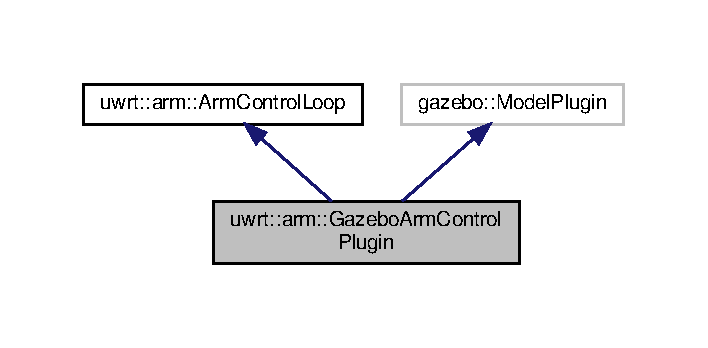
\includegraphics[width=340pt]{classuwrt_1_1arm_1_1_gazebo_arm_control_plugin__inherit__graph}
\end{center}
\end{figure}


Collaboration diagram for uwrt\+:\+:arm\+:\+:Gazebo\+Arm\+Control\+Plugin\+:
\nopagebreak
\begin{figure}[H]
\begin{center}
\leavevmode
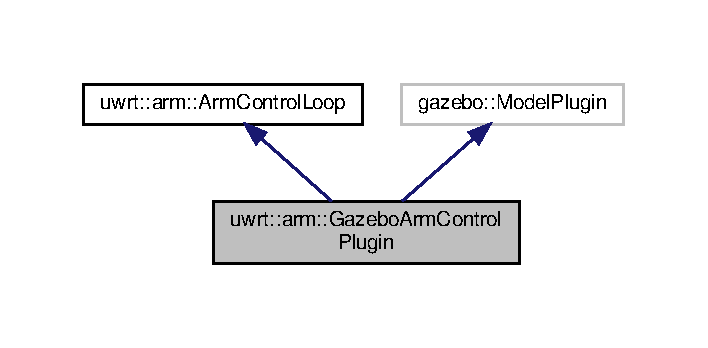
\includegraphics[width=340pt]{classuwrt_1_1arm_1_1_gazebo_arm_control_plugin__coll__graph}
\end{center}
\end{figure}
\subsection*{Public Member Functions}
\begin{DoxyCompactItemize}
\item 
\hyperlink{classuwrt_1_1arm_1_1_gazebo_arm_control_plugin_a0d74230d845e14e47d10d11636a76240}{Gazebo\+Arm\+Control\+Plugin} ()
\item 
void \hyperlink{classuwrt_1_1arm_1_1_gazebo_arm_control_plugin_a180f7cf53ddfa6d3a3afbbedc2c88bc7}{Load} (gazebo\+::physics\+::\+Model\+Ptr model, sdf\+::\+Element\+Ptr sdf) override
\item 
void \hyperlink{classuwrt_1_1arm_1_1_gazebo_arm_control_plugin_ae6f4223a75905adedd205b3f594d70d3}{Reset} () override
\item 
void \hyperlink{classuwrt_1_1arm_1_1_gazebo_arm_control_plugin_a83d2d6fb09930c43ee2bb5ab636501b1}{world\+Update} (const gazebo\+::common\+::\+Update\+Info \&info)
\end{DoxyCompactItemize}
\subsection*{Additional Inherited Members}


\subsection{Detailed Description}
Gazebo Plugin for simulated Arm Control Loop 

\subsection{Constructor \& Destructor Documentation}
\mbox{\Hypertarget{classuwrt_1_1arm_1_1_gazebo_arm_control_plugin_a0d74230d845e14e47d10d11636a76240}\label{classuwrt_1_1arm_1_1_gazebo_arm_control_plugin_a0d74230d845e14e47d10d11636a76240}} 
\index{uwrt\+::arm\+::\+Gazebo\+Arm\+Control\+Plugin@{uwrt\+::arm\+::\+Gazebo\+Arm\+Control\+Plugin}!Gazebo\+Arm\+Control\+Plugin@{Gazebo\+Arm\+Control\+Plugin}}
\index{Gazebo\+Arm\+Control\+Plugin@{Gazebo\+Arm\+Control\+Plugin}!uwrt\+::arm\+::\+Gazebo\+Arm\+Control\+Plugin@{uwrt\+::arm\+::\+Gazebo\+Arm\+Control\+Plugin}}
\subsubsection{\texorpdfstring{Gazebo\+Arm\+Control\+Plugin()}{GazeboArmControlPlugin()}}
{\footnotesize\ttfamily uwrt\+::arm\+::\+Gazebo\+Arm\+Control\+Plugin\+::\+Gazebo\+Arm\+Control\+Plugin (\begin{DoxyParamCaption}{ }\end{DoxyParamCaption})}



\subsection{Member Function Documentation}
\mbox{\Hypertarget{classuwrt_1_1arm_1_1_gazebo_arm_control_plugin_a180f7cf53ddfa6d3a3afbbedc2c88bc7}\label{classuwrt_1_1arm_1_1_gazebo_arm_control_plugin_a180f7cf53ddfa6d3a3afbbedc2c88bc7}} 
\index{uwrt\+::arm\+::\+Gazebo\+Arm\+Control\+Plugin@{uwrt\+::arm\+::\+Gazebo\+Arm\+Control\+Plugin}!Load@{Load}}
\index{Load@{Load}!uwrt\+::arm\+::\+Gazebo\+Arm\+Control\+Plugin@{uwrt\+::arm\+::\+Gazebo\+Arm\+Control\+Plugin}}
\subsubsection{\texorpdfstring{Load()}{Load()}}
{\footnotesize\ttfamily void uwrt\+::arm\+::\+Gazebo\+Arm\+Control\+Plugin\+::\+Load (\begin{DoxyParamCaption}\item[{gazebo\+::physics\+::\+Model\+Ptr}]{model,  }\item[{sdf\+::\+Element\+Ptr}]{sdf }\end{DoxyParamCaption})\hspace{0.3cm}{\ttfamily [override]}}

\mbox{\Hypertarget{classuwrt_1_1arm_1_1_gazebo_arm_control_plugin_ae6f4223a75905adedd205b3f594d70d3}\label{classuwrt_1_1arm_1_1_gazebo_arm_control_plugin_ae6f4223a75905adedd205b3f594d70d3}} 
\index{uwrt\+::arm\+::\+Gazebo\+Arm\+Control\+Plugin@{uwrt\+::arm\+::\+Gazebo\+Arm\+Control\+Plugin}!Reset@{Reset}}
\index{Reset@{Reset}!uwrt\+::arm\+::\+Gazebo\+Arm\+Control\+Plugin@{uwrt\+::arm\+::\+Gazebo\+Arm\+Control\+Plugin}}
\subsubsection{\texorpdfstring{Reset()}{Reset()}}
{\footnotesize\ttfamily void uwrt\+::arm\+::\+Gazebo\+Arm\+Control\+Plugin\+::\+Reset (\begin{DoxyParamCaption}{ }\end{DoxyParamCaption})\hspace{0.3cm}{\ttfamily [override]}}

\mbox{\Hypertarget{classuwrt_1_1arm_1_1_gazebo_arm_control_plugin_a83d2d6fb09930c43ee2bb5ab636501b1}\label{classuwrt_1_1arm_1_1_gazebo_arm_control_plugin_a83d2d6fb09930c43ee2bb5ab636501b1}} 
\index{uwrt\+::arm\+::\+Gazebo\+Arm\+Control\+Plugin@{uwrt\+::arm\+::\+Gazebo\+Arm\+Control\+Plugin}!world\+Update@{world\+Update}}
\index{world\+Update@{world\+Update}!uwrt\+::arm\+::\+Gazebo\+Arm\+Control\+Plugin@{uwrt\+::arm\+::\+Gazebo\+Arm\+Control\+Plugin}}
\subsubsection{\texorpdfstring{world\+Update()}{worldUpdate()}}
{\footnotesize\ttfamily void uwrt\+::arm\+::\+Gazebo\+Arm\+Control\+Plugin\+::world\+Update (\begin{DoxyParamCaption}\item[{const gazebo\+::common\+::\+Update\+Info \&}]{info }\end{DoxyParamCaption})}



The documentation for this class was generated from the following files\+:\begin{DoxyCompactItemize}
\item 
uwrt\+\_\+arm\+\_\+hw/include/uwrt\+\_\+arm\+\_\+hw/\hyperlink{gazebo__arm__control__plugin_8h}{gazebo\+\_\+arm\+\_\+control\+\_\+plugin.\+h}\item 
uwrt\+\_\+arm\+\_\+hw/src/\hyperlink{gazebo__arm__control__plugin_8cpp}{gazebo\+\_\+arm\+\_\+control\+\_\+plugin.\+cpp}\end{DoxyCompactItemize}

\hypertarget{structuwrt_1_1arm_1_1can__id_1_1_get}{}\section{uwrt\+:\+:arm\+:\+:can\+\_\+id\+:\+:Get Struct Reference}
\label{structuwrt_1_1arm_1_1can__id_1_1_get}\index{uwrt\+::arm\+::can\+\_\+id\+::\+Get@{uwrt\+::arm\+::can\+\_\+id\+::\+Get}}


{\ttfamily \#include $<$can\+\_\+config.\+h$>$}

\subsection*{Static Public Attributes}
\begin{DoxyCompactItemize}
\item 
static const canid\+\_\+t \hyperlink{structuwrt_1_1arm_1_1can__id_1_1_get_ac1c7b8f0e61fb15707187ec7413f3c16}{A\+R\+M\+\_\+\+E\+R\+R\+OR} = 0x100
\item 
static const canid\+\_\+t \hyperlink{structuwrt_1_1arm_1_1can__id_1_1_get_a48b3f0857a911585ea517a984cf1ae57}{T\+U\+R\+N\+T\+A\+B\+L\+E\+\_\+\+F\+E\+E\+D\+B\+A\+CK} = 0x758
\item 
static const canid\+\_\+t \hyperlink{structuwrt_1_1arm_1_1can__id_1_1_get_abf59392acead218b613b7f96033d6cc3}{S\+H\+O\+U\+L\+D\+E\+R\+\_\+\+F\+E\+E\+D\+B\+A\+CK} = 0x759
\item 
static const canid\+\_\+t \hyperlink{structuwrt_1_1arm_1_1can__id_1_1_get_aca504ea48dcf663b7cc12d03b121c0fd}{E\+L\+B\+O\+W\+\_\+\+F\+E\+E\+D\+B\+A\+CK} = 0x75A
\item 
static const canid\+\_\+t \hyperlink{structuwrt_1_1arm_1_1can__id_1_1_get_a9cff80034d39cc8bef41ff8e07eb38de}{W\+R\+I\+S\+T\+\_\+\+P\+I\+T\+C\+H\+\_\+\+F\+E\+E\+D\+B\+A\+CK} = 0x75B
\item 
static const canid\+\_\+t \hyperlink{structuwrt_1_1arm_1_1can__id_1_1_get_a62e8920aac6639c70b18b1953b590865}{W\+R\+I\+S\+T\+\_\+\+R\+O\+L\+L\+\_\+\+F\+E\+E\+D\+B\+A\+CK} = 0x75C
\item 
static const canid\+\_\+t \hyperlink{structuwrt_1_1arm_1_1can__id_1_1_get_a2481035a88034d41e6d8d3f5ce550332}{C\+L\+A\+W\+\_\+\+F\+E\+E\+D\+B\+A\+CK} = 0x75D
\item 
static const canid\+\_\+t \hyperlink{structuwrt_1_1arm_1_1can__id_1_1_get_a0d602e43d7cd1b39d96c98d8ad836966}{F\+O\+R\+C\+E\+\_\+\+S\+E\+N\+S\+O\+R\+\_\+\+V\+A\+L\+UE} = 0x75E
\end{DoxyCompactItemize}


\subsection{Detailed Description}
C\+AN I\+Ds for feedback/reads 

\subsection{Member Data Documentation}
\mbox{\Hypertarget{structuwrt_1_1arm_1_1can__id_1_1_get_ac1c7b8f0e61fb15707187ec7413f3c16}\label{structuwrt_1_1arm_1_1can__id_1_1_get_ac1c7b8f0e61fb15707187ec7413f3c16}} 
\index{uwrt\+::arm\+::can\+\_\+id\+::\+Get@{uwrt\+::arm\+::can\+\_\+id\+::\+Get}!A\+R\+M\+\_\+\+E\+R\+R\+OR@{A\+R\+M\+\_\+\+E\+R\+R\+OR}}
\index{A\+R\+M\+\_\+\+E\+R\+R\+OR@{A\+R\+M\+\_\+\+E\+R\+R\+OR}!uwrt\+::arm\+::can\+\_\+id\+::\+Get@{uwrt\+::arm\+::can\+\_\+id\+::\+Get}}
\subsubsection{\texorpdfstring{A\+R\+M\+\_\+\+E\+R\+R\+OR}{ARM\_ERROR}}
{\footnotesize\ttfamily const canid\+\_\+t uwrt\+::arm\+::can\+\_\+id\+::\+Get\+::\+A\+R\+M\+\_\+\+E\+R\+R\+OR = 0x100\hspace{0.3cm}{\ttfamily [static]}}

\mbox{\Hypertarget{structuwrt_1_1arm_1_1can__id_1_1_get_a2481035a88034d41e6d8d3f5ce550332}\label{structuwrt_1_1arm_1_1can__id_1_1_get_a2481035a88034d41e6d8d3f5ce550332}} 
\index{uwrt\+::arm\+::can\+\_\+id\+::\+Get@{uwrt\+::arm\+::can\+\_\+id\+::\+Get}!C\+L\+A\+W\+\_\+\+F\+E\+E\+D\+B\+A\+CK@{C\+L\+A\+W\+\_\+\+F\+E\+E\+D\+B\+A\+CK}}
\index{C\+L\+A\+W\+\_\+\+F\+E\+E\+D\+B\+A\+CK@{C\+L\+A\+W\+\_\+\+F\+E\+E\+D\+B\+A\+CK}!uwrt\+::arm\+::can\+\_\+id\+::\+Get@{uwrt\+::arm\+::can\+\_\+id\+::\+Get}}
\subsubsection{\texorpdfstring{C\+L\+A\+W\+\_\+\+F\+E\+E\+D\+B\+A\+CK}{CLAW\_FEEDBACK}}
{\footnotesize\ttfamily const canid\+\_\+t uwrt\+::arm\+::can\+\_\+id\+::\+Get\+::\+C\+L\+A\+W\+\_\+\+F\+E\+E\+D\+B\+A\+CK = 0x75D\hspace{0.3cm}{\ttfamily [static]}}

\mbox{\Hypertarget{structuwrt_1_1arm_1_1can__id_1_1_get_aca504ea48dcf663b7cc12d03b121c0fd}\label{structuwrt_1_1arm_1_1can__id_1_1_get_aca504ea48dcf663b7cc12d03b121c0fd}} 
\index{uwrt\+::arm\+::can\+\_\+id\+::\+Get@{uwrt\+::arm\+::can\+\_\+id\+::\+Get}!E\+L\+B\+O\+W\+\_\+\+F\+E\+E\+D\+B\+A\+CK@{E\+L\+B\+O\+W\+\_\+\+F\+E\+E\+D\+B\+A\+CK}}
\index{E\+L\+B\+O\+W\+\_\+\+F\+E\+E\+D\+B\+A\+CK@{E\+L\+B\+O\+W\+\_\+\+F\+E\+E\+D\+B\+A\+CK}!uwrt\+::arm\+::can\+\_\+id\+::\+Get@{uwrt\+::arm\+::can\+\_\+id\+::\+Get}}
\subsubsection{\texorpdfstring{E\+L\+B\+O\+W\+\_\+\+F\+E\+E\+D\+B\+A\+CK}{ELBOW\_FEEDBACK}}
{\footnotesize\ttfamily const canid\+\_\+t uwrt\+::arm\+::can\+\_\+id\+::\+Get\+::\+E\+L\+B\+O\+W\+\_\+\+F\+E\+E\+D\+B\+A\+CK = 0x75A\hspace{0.3cm}{\ttfamily [static]}}

\mbox{\Hypertarget{structuwrt_1_1arm_1_1can__id_1_1_get_a0d602e43d7cd1b39d96c98d8ad836966}\label{structuwrt_1_1arm_1_1can__id_1_1_get_a0d602e43d7cd1b39d96c98d8ad836966}} 
\index{uwrt\+::arm\+::can\+\_\+id\+::\+Get@{uwrt\+::arm\+::can\+\_\+id\+::\+Get}!F\+O\+R\+C\+E\+\_\+\+S\+E\+N\+S\+O\+R\+\_\+\+V\+A\+L\+UE@{F\+O\+R\+C\+E\+\_\+\+S\+E\+N\+S\+O\+R\+\_\+\+V\+A\+L\+UE}}
\index{F\+O\+R\+C\+E\+\_\+\+S\+E\+N\+S\+O\+R\+\_\+\+V\+A\+L\+UE@{F\+O\+R\+C\+E\+\_\+\+S\+E\+N\+S\+O\+R\+\_\+\+V\+A\+L\+UE}!uwrt\+::arm\+::can\+\_\+id\+::\+Get@{uwrt\+::arm\+::can\+\_\+id\+::\+Get}}
\subsubsection{\texorpdfstring{F\+O\+R\+C\+E\+\_\+\+S\+E\+N\+S\+O\+R\+\_\+\+V\+A\+L\+UE}{FORCE\_SENSOR\_VALUE}}
{\footnotesize\ttfamily const canid\+\_\+t uwrt\+::arm\+::can\+\_\+id\+::\+Get\+::\+F\+O\+R\+C\+E\+\_\+\+S\+E\+N\+S\+O\+R\+\_\+\+V\+A\+L\+UE = 0x75E\hspace{0.3cm}{\ttfamily [static]}}

\mbox{\Hypertarget{structuwrt_1_1arm_1_1can__id_1_1_get_abf59392acead218b613b7f96033d6cc3}\label{structuwrt_1_1arm_1_1can__id_1_1_get_abf59392acead218b613b7f96033d6cc3}} 
\index{uwrt\+::arm\+::can\+\_\+id\+::\+Get@{uwrt\+::arm\+::can\+\_\+id\+::\+Get}!S\+H\+O\+U\+L\+D\+E\+R\+\_\+\+F\+E\+E\+D\+B\+A\+CK@{S\+H\+O\+U\+L\+D\+E\+R\+\_\+\+F\+E\+E\+D\+B\+A\+CK}}
\index{S\+H\+O\+U\+L\+D\+E\+R\+\_\+\+F\+E\+E\+D\+B\+A\+CK@{S\+H\+O\+U\+L\+D\+E\+R\+\_\+\+F\+E\+E\+D\+B\+A\+CK}!uwrt\+::arm\+::can\+\_\+id\+::\+Get@{uwrt\+::arm\+::can\+\_\+id\+::\+Get}}
\subsubsection{\texorpdfstring{S\+H\+O\+U\+L\+D\+E\+R\+\_\+\+F\+E\+E\+D\+B\+A\+CK}{SHOULDER\_FEEDBACK}}
{\footnotesize\ttfamily const canid\+\_\+t uwrt\+::arm\+::can\+\_\+id\+::\+Get\+::\+S\+H\+O\+U\+L\+D\+E\+R\+\_\+\+F\+E\+E\+D\+B\+A\+CK = 0x759\hspace{0.3cm}{\ttfamily [static]}}

\mbox{\Hypertarget{structuwrt_1_1arm_1_1can__id_1_1_get_a48b3f0857a911585ea517a984cf1ae57}\label{structuwrt_1_1arm_1_1can__id_1_1_get_a48b3f0857a911585ea517a984cf1ae57}} 
\index{uwrt\+::arm\+::can\+\_\+id\+::\+Get@{uwrt\+::arm\+::can\+\_\+id\+::\+Get}!T\+U\+R\+N\+T\+A\+B\+L\+E\+\_\+\+F\+E\+E\+D\+B\+A\+CK@{T\+U\+R\+N\+T\+A\+B\+L\+E\+\_\+\+F\+E\+E\+D\+B\+A\+CK}}
\index{T\+U\+R\+N\+T\+A\+B\+L\+E\+\_\+\+F\+E\+E\+D\+B\+A\+CK@{T\+U\+R\+N\+T\+A\+B\+L\+E\+\_\+\+F\+E\+E\+D\+B\+A\+CK}!uwrt\+::arm\+::can\+\_\+id\+::\+Get@{uwrt\+::arm\+::can\+\_\+id\+::\+Get}}
\subsubsection{\texorpdfstring{T\+U\+R\+N\+T\+A\+B\+L\+E\+\_\+\+F\+E\+E\+D\+B\+A\+CK}{TURNTABLE\_FEEDBACK}}
{\footnotesize\ttfamily const canid\+\_\+t uwrt\+::arm\+::can\+\_\+id\+::\+Get\+::\+T\+U\+R\+N\+T\+A\+B\+L\+E\+\_\+\+F\+E\+E\+D\+B\+A\+CK = 0x758\hspace{0.3cm}{\ttfamily [static]}}

\mbox{\Hypertarget{structuwrt_1_1arm_1_1can__id_1_1_get_a9cff80034d39cc8bef41ff8e07eb38de}\label{structuwrt_1_1arm_1_1can__id_1_1_get_a9cff80034d39cc8bef41ff8e07eb38de}} 
\index{uwrt\+::arm\+::can\+\_\+id\+::\+Get@{uwrt\+::arm\+::can\+\_\+id\+::\+Get}!W\+R\+I\+S\+T\+\_\+\+P\+I\+T\+C\+H\+\_\+\+F\+E\+E\+D\+B\+A\+CK@{W\+R\+I\+S\+T\+\_\+\+P\+I\+T\+C\+H\+\_\+\+F\+E\+E\+D\+B\+A\+CK}}
\index{W\+R\+I\+S\+T\+\_\+\+P\+I\+T\+C\+H\+\_\+\+F\+E\+E\+D\+B\+A\+CK@{W\+R\+I\+S\+T\+\_\+\+P\+I\+T\+C\+H\+\_\+\+F\+E\+E\+D\+B\+A\+CK}!uwrt\+::arm\+::can\+\_\+id\+::\+Get@{uwrt\+::arm\+::can\+\_\+id\+::\+Get}}
\subsubsection{\texorpdfstring{W\+R\+I\+S\+T\+\_\+\+P\+I\+T\+C\+H\+\_\+\+F\+E\+E\+D\+B\+A\+CK}{WRIST\_PITCH\_FEEDBACK}}
{\footnotesize\ttfamily const canid\+\_\+t uwrt\+::arm\+::can\+\_\+id\+::\+Get\+::\+W\+R\+I\+S\+T\+\_\+\+P\+I\+T\+C\+H\+\_\+\+F\+E\+E\+D\+B\+A\+CK = 0x75B\hspace{0.3cm}{\ttfamily [static]}}

\mbox{\Hypertarget{structuwrt_1_1arm_1_1can__id_1_1_get_a62e8920aac6639c70b18b1953b590865}\label{structuwrt_1_1arm_1_1can__id_1_1_get_a62e8920aac6639c70b18b1953b590865}} 
\index{uwrt\+::arm\+::can\+\_\+id\+::\+Get@{uwrt\+::arm\+::can\+\_\+id\+::\+Get}!W\+R\+I\+S\+T\+\_\+\+R\+O\+L\+L\+\_\+\+F\+E\+E\+D\+B\+A\+CK@{W\+R\+I\+S\+T\+\_\+\+R\+O\+L\+L\+\_\+\+F\+E\+E\+D\+B\+A\+CK}}
\index{W\+R\+I\+S\+T\+\_\+\+R\+O\+L\+L\+\_\+\+F\+E\+E\+D\+B\+A\+CK@{W\+R\+I\+S\+T\+\_\+\+R\+O\+L\+L\+\_\+\+F\+E\+E\+D\+B\+A\+CK}!uwrt\+::arm\+::can\+\_\+id\+::\+Get@{uwrt\+::arm\+::can\+\_\+id\+::\+Get}}
\subsubsection{\texorpdfstring{W\+R\+I\+S\+T\+\_\+\+R\+O\+L\+L\+\_\+\+F\+E\+E\+D\+B\+A\+CK}{WRIST\_ROLL\_FEEDBACK}}
{\footnotesize\ttfamily const canid\+\_\+t uwrt\+::arm\+::can\+\_\+id\+::\+Get\+::\+W\+R\+I\+S\+T\+\_\+\+R\+O\+L\+L\+\_\+\+F\+E\+E\+D\+B\+A\+CK = 0x75C\hspace{0.3cm}{\ttfamily [static]}}



The documentation for this struct was generated from the following file\+:\begin{DoxyCompactItemize}
\item 
uwrt\+\_\+arm\+\_\+hw/include/uwrt\+\_\+arm\+\_\+hw/\hyperlink{can__config_8h}{can\+\_\+config.\+h}\end{DoxyCompactItemize}

\hypertarget{classuwrt_1_1arm_1_1_real_arm_control}{}\section{uwrt\+:\+:arm\+:\+:Real\+Arm\+Control Class Reference}
\label{classuwrt_1_1arm_1_1_real_arm_control}\index{uwrt\+::arm\+::\+Real\+Arm\+Control@{uwrt\+::arm\+::\+Real\+Arm\+Control}}


{\ttfamily \#include $<$real\+\_\+arm\+\_\+control.\+h$>$}



Inheritance diagram for uwrt\+:\+:arm\+:\+:Real\+Arm\+Control\+:
\nopagebreak
\begin{figure}[H]
\begin{center}
\leavevmode
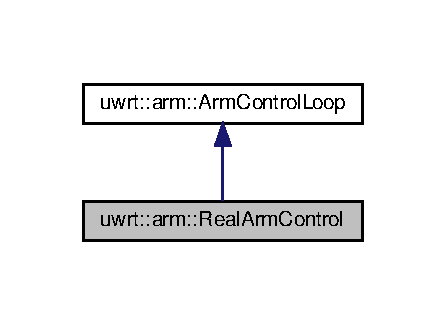
\includegraphics[width=214pt]{classuwrt_1_1arm_1_1_real_arm_control__inherit__graph}
\end{center}
\end{figure}


Collaboration diagram for uwrt\+:\+:arm\+:\+:Real\+Arm\+Control\+:
\nopagebreak
\begin{figure}[H]
\begin{center}
\leavevmode
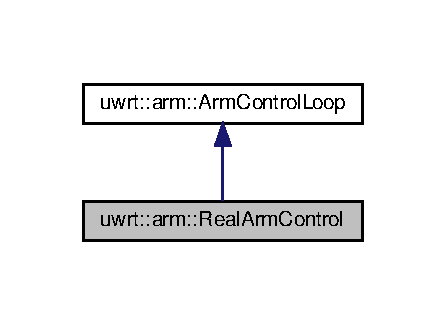
\includegraphics[width=214pt]{classuwrt_1_1arm_1_1_real_arm_control__coll__graph}
\end{center}
\end{figure}
\subsection*{Public Member Functions}
\begin{DoxyCompactItemize}
\item 
\hyperlink{classuwrt_1_1arm_1_1_real_arm_control_aedb0ce5a7ad8b1e8451806873544c00d}{Real\+Arm\+Control} ()
\begin{DoxyCompactList}\small\item\em Constructor. \end{DoxyCompactList}\item 
\hyperlink{classuwrt_1_1arm_1_1_real_arm_control_a1f201262f19bfae812e33d4ce47f9ba2}{$\sim$\+Real\+Arm\+Control} ()
\begin{DoxyCompactList}\small\item\em Destructor. \end{DoxyCompactList}\item 
void \hyperlink{classuwrt_1_1arm_1_1_real_arm_control_aa6b49ca2736508e70b4b135c21f1cf51}{spin\+Once} ()
\begin{DoxyCompactList}\small\item\em Read, Write and perform controller updates based on control period. \end{DoxyCompactList}\item 
void \hyperlink{classuwrt_1_1arm_1_1_real_arm_control_ac174f649dd8c5a48250e0b84b4442b5e}{spin} ()
\end{DoxyCompactItemize}
\subsection*{Additional Inherited Members}


\subsection{Detailed Description}
Arm Control Loop for the real Arm hardware 

\subsection{Constructor \& Destructor Documentation}
\mbox{\Hypertarget{classuwrt_1_1arm_1_1_real_arm_control_aedb0ce5a7ad8b1e8451806873544c00d}\label{classuwrt_1_1arm_1_1_real_arm_control_aedb0ce5a7ad8b1e8451806873544c00d}} 
\index{uwrt\+::arm\+::\+Real\+Arm\+Control@{uwrt\+::arm\+::\+Real\+Arm\+Control}!Real\+Arm\+Control@{Real\+Arm\+Control}}
\index{Real\+Arm\+Control@{Real\+Arm\+Control}!uwrt\+::arm\+::\+Real\+Arm\+Control@{uwrt\+::arm\+::\+Real\+Arm\+Control}}
\subsubsection{\texorpdfstring{Real\+Arm\+Control()}{RealArmControl()}}
{\footnotesize\ttfamily uwrt\+::arm\+::\+Real\+Arm\+Control\+::\+Real\+Arm\+Control (\begin{DoxyParamCaption}{ }\end{DoxyParamCaption})}



Constructor. 

\mbox{\Hypertarget{classuwrt_1_1arm_1_1_real_arm_control_a1f201262f19bfae812e33d4ce47f9ba2}\label{classuwrt_1_1arm_1_1_real_arm_control_a1f201262f19bfae812e33d4ce47f9ba2}} 
\index{uwrt\+::arm\+::\+Real\+Arm\+Control@{uwrt\+::arm\+::\+Real\+Arm\+Control}!````~Real\+Arm\+Control@{$\sim$\+Real\+Arm\+Control}}
\index{````~Real\+Arm\+Control@{$\sim$\+Real\+Arm\+Control}!uwrt\+::arm\+::\+Real\+Arm\+Control@{uwrt\+::arm\+::\+Real\+Arm\+Control}}
\subsubsection{\texorpdfstring{$\sim$\+Real\+Arm\+Control()}{~RealArmControl()}}
{\footnotesize\ttfamily uwrt\+::arm\+::\+Real\+Arm\+Control\+::$\sim$\+Real\+Arm\+Control (\begin{DoxyParamCaption}{ }\end{DoxyParamCaption})}



Destructor. 



\subsection{Member Function Documentation}
\mbox{\Hypertarget{classuwrt_1_1arm_1_1_real_arm_control_ac174f649dd8c5a48250e0b84b4442b5e}\label{classuwrt_1_1arm_1_1_real_arm_control_ac174f649dd8c5a48250e0b84b4442b5e}} 
\index{uwrt\+::arm\+::\+Real\+Arm\+Control@{uwrt\+::arm\+::\+Real\+Arm\+Control}!spin@{spin}}
\index{spin@{spin}!uwrt\+::arm\+::\+Real\+Arm\+Control@{uwrt\+::arm\+::\+Real\+Arm\+Control}}
\subsubsection{\texorpdfstring{spin()}{spin()}}
{\footnotesize\ttfamily void uwrt\+::arm\+::\+Real\+Arm\+Control\+::spin (\begin{DoxyParamCaption}{ }\end{DoxyParamCaption})}

Blocking loop of reads, writes and controller updates \mbox{\Hypertarget{classuwrt_1_1arm_1_1_real_arm_control_aa6b49ca2736508e70b4b135c21f1cf51}\label{classuwrt_1_1arm_1_1_real_arm_control_aa6b49ca2736508e70b4b135c21f1cf51}} 
\index{uwrt\+::arm\+::\+Real\+Arm\+Control@{uwrt\+::arm\+::\+Real\+Arm\+Control}!spin\+Once@{spin\+Once}}
\index{spin\+Once@{spin\+Once}!uwrt\+::arm\+::\+Real\+Arm\+Control@{uwrt\+::arm\+::\+Real\+Arm\+Control}}
\subsubsection{\texorpdfstring{spin\+Once()}{spinOnce()}}
{\footnotesize\ttfamily void uwrt\+::arm\+::\+Real\+Arm\+Control\+::spin\+Once (\begin{DoxyParamCaption}{ }\end{DoxyParamCaption})}



Read, Write and perform controller updates based on control period. 



The documentation for this class was generated from the following files\+:\begin{DoxyCompactItemize}
\item 
uwrt\+\_\+arm\+\_\+hw/include/uwrt\+\_\+arm\+\_\+hw/\hyperlink{real__arm__control_8h}{real\+\_\+arm\+\_\+control.\+h}\item 
uwrt\+\_\+arm\+\_\+hw/src/\hyperlink{real__arm__control_8cpp}{real\+\_\+arm\+\_\+control.\+cpp}\end{DoxyCompactItemize}

\hypertarget{structuwrt_1_1arm_1_1can__id_1_1_set}{}\section{uwrt\+:\+:arm\+:\+:can\+\_\+id\+:\+:Set Struct Reference}
\label{structuwrt_1_1arm_1_1can__id_1_1_set}\index{uwrt\+::arm\+::can\+\_\+id\+::\+Set@{uwrt\+::arm\+::can\+\_\+id\+::\+Set}}


{\ttfamily \#include $<$can\+\_\+config.\+h$>$}

\subsection*{Static Public Attributes}
\begin{DoxyCompactItemize}
\item 
static const canid\+\_\+t \hyperlink{structuwrt_1_1arm_1_1can__id_1_1_set_a003226a9e1602b02671aa2c7238d6e39}{T\+U\+R\+N\+T\+A\+B\+L\+E\+\_\+\+C\+O\+N\+T\+R\+O\+L\+\_\+\+M\+O\+DE} = 0x740
\item 
static const canid\+\_\+t \hyperlink{structuwrt_1_1arm_1_1can__id_1_1_set_aa9f008380317a3e374cedb991f2b7c0c}{S\+H\+O\+U\+L\+D\+E\+R\+\_\+\+C\+O\+N\+T\+R\+O\+L\+\_\+\+M\+O\+DE} = 0x741
\item 
static const canid\+\_\+t \hyperlink{structuwrt_1_1arm_1_1can__id_1_1_set_a7bdb4b8618186b0d9c616582384e7305}{E\+L\+B\+O\+W\+\_\+\+C\+O\+N\+T\+R\+O\+L\+\_\+\+M\+O\+DE} = 0x742
\item 
static const canid\+\_\+t \hyperlink{structuwrt_1_1arm_1_1can__id_1_1_set_a60df1e7ff2760a8b8cecc2ede18454e4}{W\+R\+I\+S\+T\+\_\+\+C\+O\+N\+T\+R\+O\+L\+\_\+\+M\+O\+DE} = 0x743
\item 
static const canid\+\_\+t \hyperlink{structuwrt_1_1arm_1_1can__id_1_1_set_aa8eb176701392e03f94bf851011a7c1d}{C\+L\+A\+W\+\_\+\+C\+O\+N\+T\+R\+O\+L\+\_\+\+M\+O\+DE} = 0x744
\item 
static const canid\+\_\+t \hyperlink{structuwrt_1_1arm_1_1can__id_1_1_set_ad0a6e521cd2d3d1b9845d1edf07d0461}{T\+U\+R\+N\+T\+A\+B\+L\+E\+\_\+\+C\+O\+M\+M\+A\+ND} = 0x745
\item 
static const canid\+\_\+t \hyperlink{structuwrt_1_1arm_1_1can__id_1_1_set_a33395d02979aedb2da0e2ea4436b2deb}{S\+H\+O\+U\+L\+D\+E\+R\+\_\+\+C\+O\+M\+M\+A\+ND} = 0x746
\item 
static const canid\+\_\+t \hyperlink{structuwrt_1_1arm_1_1can__id_1_1_set_a50d81398d123d4d37836639322a1d34c}{E\+L\+B\+O\+W\+\_\+\+C\+O\+M\+M\+A\+ND} = 0x747
\item 
static const canid\+\_\+t \hyperlink{structuwrt_1_1arm_1_1can__id_1_1_set_afa2c88815d5c513ee325da83a685f446}{W\+R\+I\+S\+T\+\_\+\+P\+I\+T\+C\+H\+\_\+\+C\+O\+M\+M\+A\+ND} = 0x748
\item 
static const canid\+\_\+t \hyperlink{structuwrt_1_1arm_1_1can__id_1_1_set_a16739ab7600b94c74d80983923f26434}{W\+R\+I\+S\+T\+\_\+\+R\+O\+L\+L\+\_\+\+C\+O\+M\+M\+A\+ND} = 0x749
\item 
static const canid\+\_\+t \hyperlink{structuwrt_1_1arm_1_1can__id_1_1_set_a04c95641da03af9913aaf4c7b2014d2b}{C\+L\+A\+W\+\_\+\+C\+O\+M\+M\+A\+ND} = 0x74A
\item 
static const canid\+\_\+t \hyperlink{structuwrt_1_1arm_1_1can__id_1_1_set_a30a32e87691781dc9d6cc34175a4bf06}{T\+O\+O\+L\+T\+I\+P\+\_\+\+D\+E\+P\+L\+OY} = 0x74B
\item 
static const canid\+\_\+t \hyperlink{structuwrt_1_1arm_1_1can__id_1_1_set_a77e9a4a1f79b8edbff6712a7d70083bb}{P\+I\+D\+\_\+\+T\+U\+N\+I\+N\+G\+\_\+\+M\+O\+DE} = 0x750
\item 
static const canid\+\_\+t \hyperlink{structuwrt_1_1arm_1_1can__id_1_1_set_ab5a1f00f9ce98c896671623f007ff45a}{P\+I\+D\+\_\+\+D\+E\+A\+D\+Z\+O\+NE} = 0x751
\item 
static const canid\+\_\+t \hyperlink{structuwrt_1_1arm_1_1can__id_1_1_set_ab666f9f830c47bb25c21017495a2b8fd}{P\+I\+D\+\_\+P} = 0x752
\item 
static const canid\+\_\+t \hyperlink{structuwrt_1_1arm_1_1can__id_1_1_set_a58a1c4a1ca8419e1811ff9df15184535}{P\+I\+D\+\_\+I} = 0x753
\item 
static const canid\+\_\+t \hyperlink{structuwrt_1_1arm_1_1can__id_1_1_set_a12d83aa98072fc84f1c5c04a6e8b98e8}{P\+I\+D\+\_\+D} = 0x754
\item 
static const canid\+\_\+t \hyperlink{structuwrt_1_1arm_1_1can__id_1_1_set_a57dc39813fe5a8bee6022c44a7c64e75}{P\+I\+D\+\_\+\+B\+I\+AS} = 0x755
\end{DoxyCompactItemize}


\subsection{Detailed Description}
C\+AN I\+Ds for commands/writes 

\subsection{Member Data Documentation}
\mbox{\Hypertarget{structuwrt_1_1arm_1_1can__id_1_1_set_a04c95641da03af9913aaf4c7b2014d2b}\label{structuwrt_1_1arm_1_1can__id_1_1_set_a04c95641da03af9913aaf4c7b2014d2b}} 
\index{uwrt\+::arm\+::can\+\_\+id\+::\+Set@{uwrt\+::arm\+::can\+\_\+id\+::\+Set}!C\+L\+A\+W\+\_\+\+C\+O\+M\+M\+A\+ND@{C\+L\+A\+W\+\_\+\+C\+O\+M\+M\+A\+ND}}
\index{C\+L\+A\+W\+\_\+\+C\+O\+M\+M\+A\+ND@{C\+L\+A\+W\+\_\+\+C\+O\+M\+M\+A\+ND}!uwrt\+::arm\+::can\+\_\+id\+::\+Set@{uwrt\+::arm\+::can\+\_\+id\+::\+Set}}
\subsubsection{\texorpdfstring{C\+L\+A\+W\+\_\+\+C\+O\+M\+M\+A\+ND}{CLAW\_COMMAND}}
{\footnotesize\ttfamily const canid\+\_\+t uwrt\+::arm\+::can\+\_\+id\+::\+Set\+::\+C\+L\+A\+W\+\_\+\+C\+O\+M\+M\+A\+ND = 0x74A\hspace{0.3cm}{\ttfamily [static]}}

\mbox{\Hypertarget{structuwrt_1_1arm_1_1can__id_1_1_set_aa8eb176701392e03f94bf851011a7c1d}\label{structuwrt_1_1arm_1_1can__id_1_1_set_aa8eb176701392e03f94bf851011a7c1d}} 
\index{uwrt\+::arm\+::can\+\_\+id\+::\+Set@{uwrt\+::arm\+::can\+\_\+id\+::\+Set}!C\+L\+A\+W\+\_\+\+C\+O\+N\+T\+R\+O\+L\+\_\+\+M\+O\+DE@{C\+L\+A\+W\+\_\+\+C\+O\+N\+T\+R\+O\+L\+\_\+\+M\+O\+DE}}
\index{C\+L\+A\+W\+\_\+\+C\+O\+N\+T\+R\+O\+L\+\_\+\+M\+O\+DE@{C\+L\+A\+W\+\_\+\+C\+O\+N\+T\+R\+O\+L\+\_\+\+M\+O\+DE}!uwrt\+::arm\+::can\+\_\+id\+::\+Set@{uwrt\+::arm\+::can\+\_\+id\+::\+Set}}
\subsubsection{\texorpdfstring{C\+L\+A\+W\+\_\+\+C\+O\+N\+T\+R\+O\+L\+\_\+\+M\+O\+DE}{CLAW\_CONTROL\_MODE}}
{\footnotesize\ttfamily const canid\+\_\+t uwrt\+::arm\+::can\+\_\+id\+::\+Set\+::\+C\+L\+A\+W\+\_\+\+C\+O\+N\+T\+R\+O\+L\+\_\+\+M\+O\+DE = 0x744\hspace{0.3cm}{\ttfamily [static]}}

\mbox{\Hypertarget{structuwrt_1_1arm_1_1can__id_1_1_set_a50d81398d123d4d37836639322a1d34c}\label{structuwrt_1_1arm_1_1can__id_1_1_set_a50d81398d123d4d37836639322a1d34c}} 
\index{uwrt\+::arm\+::can\+\_\+id\+::\+Set@{uwrt\+::arm\+::can\+\_\+id\+::\+Set}!E\+L\+B\+O\+W\+\_\+\+C\+O\+M\+M\+A\+ND@{E\+L\+B\+O\+W\+\_\+\+C\+O\+M\+M\+A\+ND}}
\index{E\+L\+B\+O\+W\+\_\+\+C\+O\+M\+M\+A\+ND@{E\+L\+B\+O\+W\+\_\+\+C\+O\+M\+M\+A\+ND}!uwrt\+::arm\+::can\+\_\+id\+::\+Set@{uwrt\+::arm\+::can\+\_\+id\+::\+Set}}
\subsubsection{\texorpdfstring{E\+L\+B\+O\+W\+\_\+\+C\+O\+M\+M\+A\+ND}{ELBOW\_COMMAND}}
{\footnotesize\ttfamily const canid\+\_\+t uwrt\+::arm\+::can\+\_\+id\+::\+Set\+::\+E\+L\+B\+O\+W\+\_\+\+C\+O\+M\+M\+A\+ND = 0x747\hspace{0.3cm}{\ttfamily [static]}}

\mbox{\Hypertarget{structuwrt_1_1arm_1_1can__id_1_1_set_a7bdb4b8618186b0d9c616582384e7305}\label{structuwrt_1_1arm_1_1can__id_1_1_set_a7bdb4b8618186b0d9c616582384e7305}} 
\index{uwrt\+::arm\+::can\+\_\+id\+::\+Set@{uwrt\+::arm\+::can\+\_\+id\+::\+Set}!E\+L\+B\+O\+W\+\_\+\+C\+O\+N\+T\+R\+O\+L\+\_\+\+M\+O\+DE@{E\+L\+B\+O\+W\+\_\+\+C\+O\+N\+T\+R\+O\+L\+\_\+\+M\+O\+DE}}
\index{E\+L\+B\+O\+W\+\_\+\+C\+O\+N\+T\+R\+O\+L\+\_\+\+M\+O\+DE@{E\+L\+B\+O\+W\+\_\+\+C\+O\+N\+T\+R\+O\+L\+\_\+\+M\+O\+DE}!uwrt\+::arm\+::can\+\_\+id\+::\+Set@{uwrt\+::arm\+::can\+\_\+id\+::\+Set}}
\subsubsection{\texorpdfstring{E\+L\+B\+O\+W\+\_\+\+C\+O\+N\+T\+R\+O\+L\+\_\+\+M\+O\+DE}{ELBOW\_CONTROL\_MODE}}
{\footnotesize\ttfamily const canid\+\_\+t uwrt\+::arm\+::can\+\_\+id\+::\+Set\+::\+E\+L\+B\+O\+W\+\_\+\+C\+O\+N\+T\+R\+O\+L\+\_\+\+M\+O\+DE = 0x742\hspace{0.3cm}{\ttfamily [static]}}

\mbox{\Hypertarget{structuwrt_1_1arm_1_1can__id_1_1_set_a57dc39813fe5a8bee6022c44a7c64e75}\label{structuwrt_1_1arm_1_1can__id_1_1_set_a57dc39813fe5a8bee6022c44a7c64e75}} 
\index{uwrt\+::arm\+::can\+\_\+id\+::\+Set@{uwrt\+::arm\+::can\+\_\+id\+::\+Set}!P\+I\+D\+\_\+\+B\+I\+AS@{P\+I\+D\+\_\+\+B\+I\+AS}}
\index{P\+I\+D\+\_\+\+B\+I\+AS@{P\+I\+D\+\_\+\+B\+I\+AS}!uwrt\+::arm\+::can\+\_\+id\+::\+Set@{uwrt\+::arm\+::can\+\_\+id\+::\+Set}}
\subsubsection{\texorpdfstring{P\+I\+D\+\_\+\+B\+I\+AS}{PID\_BIAS}}
{\footnotesize\ttfamily const canid\+\_\+t uwrt\+::arm\+::can\+\_\+id\+::\+Set\+::\+P\+I\+D\+\_\+\+B\+I\+AS = 0x755\hspace{0.3cm}{\ttfamily [static]}}

\mbox{\Hypertarget{structuwrt_1_1arm_1_1can__id_1_1_set_a12d83aa98072fc84f1c5c04a6e8b98e8}\label{structuwrt_1_1arm_1_1can__id_1_1_set_a12d83aa98072fc84f1c5c04a6e8b98e8}} 
\index{uwrt\+::arm\+::can\+\_\+id\+::\+Set@{uwrt\+::arm\+::can\+\_\+id\+::\+Set}!P\+I\+D\+\_\+D@{P\+I\+D\+\_\+D}}
\index{P\+I\+D\+\_\+D@{P\+I\+D\+\_\+D}!uwrt\+::arm\+::can\+\_\+id\+::\+Set@{uwrt\+::arm\+::can\+\_\+id\+::\+Set}}
\subsubsection{\texorpdfstring{P\+I\+D\+\_\+D}{PID\_D}}
{\footnotesize\ttfamily const canid\+\_\+t uwrt\+::arm\+::can\+\_\+id\+::\+Set\+::\+P\+I\+D\+\_\+D = 0x754\hspace{0.3cm}{\ttfamily [static]}}

\mbox{\Hypertarget{structuwrt_1_1arm_1_1can__id_1_1_set_ab5a1f00f9ce98c896671623f007ff45a}\label{structuwrt_1_1arm_1_1can__id_1_1_set_ab5a1f00f9ce98c896671623f007ff45a}} 
\index{uwrt\+::arm\+::can\+\_\+id\+::\+Set@{uwrt\+::arm\+::can\+\_\+id\+::\+Set}!P\+I\+D\+\_\+\+D\+E\+A\+D\+Z\+O\+NE@{P\+I\+D\+\_\+\+D\+E\+A\+D\+Z\+O\+NE}}
\index{P\+I\+D\+\_\+\+D\+E\+A\+D\+Z\+O\+NE@{P\+I\+D\+\_\+\+D\+E\+A\+D\+Z\+O\+NE}!uwrt\+::arm\+::can\+\_\+id\+::\+Set@{uwrt\+::arm\+::can\+\_\+id\+::\+Set}}
\subsubsection{\texorpdfstring{P\+I\+D\+\_\+\+D\+E\+A\+D\+Z\+O\+NE}{PID\_DEADZONE}}
{\footnotesize\ttfamily const canid\+\_\+t uwrt\+::arm\+::can\+\_\+id\+::\+Set\+::\+P\+I\+D\+\_\+\+D\+E\+A\+D\+Z\+O\+NE = 0x751\hspace{0.3cm}{\ttfamily [static]}}

\mbox{\Hypertarget{structuwrt_1_1arm_1_1can__id_1_1_set_a58a1c4a1ca8419e1811ff9df15184535}\label{structuwrt_1_1arm_1_1can__id_1_1_set_a58a1c4a1ca8419e1811ff9df15184535}} 
\index{uwrt\+::arm\+::can\+\_\+id\+::\+Set@{uwrt\+::arm\+::can\+\_\+id\+::\+Set}!P\+I\+D\+\_\+I@{P\+I\+D\+\_\+I}}
\index{P\+I\+D\+\_\+I@{P\+I\+D\+\_\+I}!uwrt\+::arm\+::can\+\_\+id\+::\+Set@{uwrt\+::arm\+::can\+\_\+id\+::\+Set}}
\subsubsection{\texorpdfstring{P\+I\+D\+\_\+I}{PID\_I}}
{\footnotesize\ttfamily const canid\+\_\+t uwrt\+::arm\+::can\+\_\+id\+::\+Set\+::\+P\+I\+D\+\_\+I = 0x753\hspace{0.3cm}{\ttfamily [static]}}

\mbox{\Hypertarget{structuwrt_1_1arm_1_1can__id_1_1_set_ab666f9f830c47bb25c21017495a2b8fd}\label{structuwrt_1_1arm_1_1can__id_1_1_set_ab666f9f830c47bb25c21017495a2b8fd}} 
\index{uwrt\+::arm\+::can\+\_\+id\+::\+Set@{uwrt\+::arm\+::can\+\_\+id\+::\+Set}!P\+I\+D\+\_\+P@{P\+I\+D\+\_\+P}}
\index{P\+I\+D\+\_\+P@{P\+I\+D\+\_\+P}!uwrt\+::arm\+::can\+\_\+id\+::\+Set@{uwrt\+::arm\+::can\+\_\+id\+::\+Set}}
\subsubsection{\texorpdfstring{P\+I\+D\+\_\+P}{PID\_P}}
{\footnotesize\ttfamily const canid\+\_\+t uwrt\+::arm\+::can\+\_\+id\+::\+Set\+::\+P\+I\+D\+\_\+P = 0x752\hspace{0.3cm}{\ttfamily [static]}}

\mbox{\Hypertarget{structuwrt_1_1arm_1_1can__id_1_1_set_a77e9a4a1f79b8edbff6712a7d70083bb}\label{structuwrt_1_1arm_1_1can__id_1_1_set_a77e9a4a1f79b8edbff6712a7d70083bb}} 
\index{uwrt\+::arm\+::can\+\_\+id\+::\+Set@{uwrt\+::arm\+::can\+\_\+id\+::\+Set}!P\+I\+D\+\_\+\+T\+U\+N\+I\+N\+G\+\_\+\+M\+O\+DE@{P\+I\+D\+\_\+\+T\+U\+N\+I\+N\+G\+\_\+\+M\+O\+DE}}
\index{P\+I\+D\+\_\+\+T\+U\+N\+I\+N\+G\+\_\+\+M\+O\+DE@{P\+I\+D\+\_\+\+T\+U\+N\+I\+N\+G\+\_\+\+M\+O\+DE}!uwrt\+::arm\+::can\+\_\+id\+::\+Set@{uwrt\+::arm\+::can\+\_\+id\+::\+Set}}
\subsubsection{\texorpdfstring{P\+I\+D\+\_\+\+T\+U\+N\+I\+N\+G\+\_\+\+M\+O\+DE}{PID\_TUNING\_MODE}}
{\footnotesize\ttfamily const canid\+\_\+t uwrt\+::arm\+::can\+\_\+id\+::\+Set\+::\+P\+I\+D\+\_\+\+T\+U\+N\+I\+N\+G\+\_\+\+M\+O\+DE = 0x750\hspace{0.3cm}{\ttfamily [static]}}

\mbox{\Hypertarget{structuwrt_1_1arm_1_1can__id_1_1_set_a33395d02979aedb2da0e2ea4436b2deb}\label{structuwrt_1_1arm_1_1can__id_1_1_set_a33395d02979aedb2da0e2ea4436b2deb}} 
\index{uwrt\+::arm\+::can\+\_\+id\+::\+Set@{uwrt\+::arm\+::can\+\_\+id\+::\+Set}!S\+H\+O\+U\+L\+D\+E\+R\+\_\+\+C\+O\+M\+M\+A\+ND@{S\+H\+O\+U\+L\+D\+E\+R\+\_\+\+C\+O\+M\+M\+A\+ND}}
\index{S\+H\+O\+U\+L\+D\+E\+R\+\_\+\+C\+O\+M\+M\+A\+ND@{S\+H\+O\+U\+L\+D\+E\+R\+\_\+\+C\+O\+M\+M\+A\+ND}!uwrt\+::arm\+::can\+\_\+id\+::\+Set@{uwrt\+::arm\+::can\+\_\+id\+::\+Set}}
\subsubsection{\texorpdfstring{S\+H\+O\+U\+L\+D\+E\+R\+\_\+\+C\+O\+M\+M\+A\+ND}{SHOULDER\_COMMAND}}
{\footnotesize\ttfamily const canid\+\_\+t uwrt\+::arm\+::can\+\_\+id\+::\+Set\+::\+S\+H\+O\+U\+L\+D\+E\+R\+\_\+\+C\+O\+M\+M\+A\+ND = 0x746\hspace{0.3cm}{\ttfamily [static]}}

\mbox{\Hypertarget{structuwrt_1_1arm_1_1can__id_1_1_set_aa9f008380317a3e374cedb991f2b7c0c}\label{structuwrt_1_1arm_1_1can__id_1_1_set_aa9f008380317a3e374cedb991f2b7c0c}} 
\index{uwrt\+::arm\+::can\+\_\+id\+::\+Set@{uwrt\+::arm\+::can\+\_\+id\+::\+Set}!S\+H\+O\+U\+L\+D\+E\+R\+\_\+\+C\+O\+N\+T\+R\+O\+L\+\_\+\+M\+O\+DE@{S\+H\+O\+U\+L\+D\+E\+R\+\_\+\+C\+O\+N\+T\+R\+O\+L\+\_\+\+M\+O\+DE}}
\index{S\+H\+O\+U\+L\+D\+E\+R\+\_\+\+C\+O\+N\+T\+R\+O\+L\+\_\+\+M\+O\+DE@{S\+H\+O\+U\+L\+D\+E\+R\+\_\+\+C\+O\+N\+T\+R\+O\+L\+\_\+\+M\+O\+DE}!uwrt\+::arm\+::can\+\_\+id\+::\+Set@{uwrt\+::arm\+::can\+\_\+id\+::\+Set}}
\subsubsection{\texorpdfstring{S\+H\+O\+U\+L\+D\+E\+R\+\_\+\+C\+O\+N\+T\+R\+O\+L\+\_\+\+M\+O\+DE}{SHOULDER\_CONTROL\_MODE}}
{\footnotesize\ttfamily const canid\+\_\+t uwrt\+::arm\+::can\+\_\+id\+::\+Set\+::\+S\+H\+O\+U\+L\+D\+E\+R\+\_\+\+C\+O\+N\+T\+R\+O\+L\+\_\+\+M\+O\+DE = 0x741\hspace{0.3cm}{\ttfamily [static]}}

\mbox{\Hypertarget{structuwrt_1_1arm_1_1can__id_1_1_set_a30a32e87691781dc9d6cc34175a4bf06}\label{structuwrt_1_1arm_1_1can__id_1_1_set_a30a32e87691781dc9d6cc34175a4bf06}} 
\index{uwrt\+::arm\+::can\+\_\+id\+::\+Set@{uwrt\+::arm\+::can\+\_\+id\+::\+Set}!T\+O\+O\+L\+T\+I\+P\+\_\+\+D\+E\+P\+L\+OY@{T\+O\+O\+L\+T\+I\+P\+\_\+\+D\+E\+P\+L\+OY}}
\index{T\+O\+O\+L\+T\+I\+P\+\_\+\+D\+E\+P\+L\+OY@{T\+O\+O\+L\+T\+I\+P\+\_\+\+D\+E\+P\+L\+OY}!uwrt\+::arm\+::can\+\_\+id\+::\+Set@{uwrt\+::arm\+::can\+\_\+id\+::\+Set}}
\subsubsection{\texorpdfstring{T\+O\+O\+L\+T\+I\+P\+\_\+\+D\+E\+P\+L\+OY}{TOOLTIP\_DEPLOY}}
{\footnotesize\ttfamily const canid\+\_\+t uwrt\+::arm\+::can\+\_\+id\+::\+Set\+::\+T\+O\+O\+L\+T\+I\+P\+\_\+\+D\+E\+P\+L\+OY = 0x74B\hspace{0.3cm}{\ttfamily [static]}}

\mbox{\Hypertarget{structuwrt_1_1arm_1_1can__id_1_1_set_ad0a6e521cd2d3d1b9845d1edf07d0461}\label{structuwrt_1_1arm_1_1can__id_1_1_set_ad0a6e521cd2d3d1b9845d1edf07d0461}} 
\index{uwrt\+::arm\+::can\+\_\+id\+::\+Set@{uwrt\+::arm\+::can\+\_\+id\+::\+Set}!T\+U\+R\+N\+T\+A\+B\+L\+E\+\_\+\+C\+O\+M\+M\+A\+ND@{T\+U\+R\+N\+T\+A\+B\+L\+E\+\_\+\+C\+O\+M\+M\+A\+ND}}
\index{T\+U\+R\+N\+T\+A\+B\+L\+E\+\_\+\+C\+O\+M\+M\+A\+ND@{T\+U\+R\+N\+T\+A\+B\+L\+E\+\_\+\+C\+O\+M\+M\+A\+ND}!uwrt\+::arm\+::can\+\_\+id\+::\+Set@{uwrt\+::arm\+::can\+\_\+id\+::\+Set}}
\subsubsection{\texorpdfstring{T\+U\+R\+N\+T\+A\+B\+L\+E\+\_\+\+C\+O\+M\+M\+A\+ND}{TURNTABLE\_COMMAND}}
{\footnotesize\ttfamily const canid\+\_\+t uwrt\+::arm\+::can\+\_\+id\+::\+Set\+::\+T\+U\+R\+N\+T\+A\+B\+L\+E\+\_\+\+C\+O\+M\+M\+A\+ND = 0x745\hspace{0.3cm}{\ttfamily [static]}}

\mbox{\Hypertarget{structuwrt_1_1arm_1_1can__id_1_1_set_a003226a9e1602b02671aa2c7238d6e39}\label{structuwrt_1_1arm_1_1can__id_1_1_set_a003226a9e1602b02671aa2c7238d6e39}} 
\index{uwrt\+::arm\+::can\+\_\+id\+::\+Set@{uwrt\+::arm\+::can\+\_\+id\+::\+Set}!T\+U\+R\+N\+T\+A\+B\+L\+E\+\_\+\+C\+O\+N\+T\+R\+O\+L\+\_\+\+M\+O\+DE@{T\+U\+R\+N\+T\+A\+B\+L\+E\+\_\+\+C\+O\+N\+T\+R\+O\+L\+\_\+\+M\+O\+DE}}
\index{T\+U\+R\+N\+T\+A\+B\+L\+E\+\_\+\+C\+O\+N\+T\+R\+O\+L\+\_\+\+M\+O\+DE@{T\+U\+R\+N\+T\+A\+B\+L\+E\+\_\+\+C\+O\+N\+T\+R\+O\+L\+\_\+\+M\+O\+DE}!uwrt\+::arm\+::can\+\_\+id\+::\+Set@{uwrt\+::arm\+::can\+\_\+id\+::\+Set}}
\subsubsection{\texorpdfstring{T\+U\+R\+N\+T\+A\+B\+L\+E\+\_\+\+C\+O\+N\+T\+R\+O\+L\+\_\+\+M\+O\+DE}{TURNTABLE\_CONTROL\_MODE}}
{\footnotesize\ttfamily const canid\+\_\+t uwrt\+::arm\+::can\+\_\+id\+::\+Set\+::\+T\+U\+R\+N\+T\+A\+B\+L\+E\+\_\+\+C\+O\+N\+T\+R\+O\+L\+\_\+\+M\+O\+DE = 0x740\hspace{0.3cm}{\ttfamily [static]}}

\mbox{\Hypertarget{structuwrt_1_1arm_1_1can__id_1_1_set_a60df1e7ff2760a8b8cecc2ede18454e4}\label{structuwrt_1_1arm_1_1can__id_1_1_set_a60df1e7ff2760a8b8cecc2ede18454e4}} 
\index{uwrt\+::arm\+::can\+\_\+id\+::\+Set@{uwrt\+::arm\+::can\+\_\+id\+::\+Set}!W\+R\+I\+S\+T\+\_\+\+C\+O\+N\+T\+R\+O\+L\+\_\+\+M\+O\+DE@{W\+R\+I\+S\+T\+\_\+\+C\+O\+N\+T\+R\+O\+L\+\_\+\+M\+O\+DE}}
\index{W\+R\+I\+S\+T\+\_\+\+C\+O\+N\+T\+R\+O\+L\+\_\+\+M\+O\+DE@{W\+R\+I\+S\+T\+\_\+\+C\+O\+N\+T\+R\+O\+L\+\_\+\+M\+O\+DE}!uwrt\+::arm\+::can\+\_\+id\+::\+Set@{uwrt\+::arm\+::can\+\_\+id\+::\+Set}}
\subsubsection{\texorpdfstring{W\+R\+I\+S\+T\+\_\+\+C\+O\+N\+T\+R\+O\+L\+\_\+\+M\+O\+DE}{WRIST\_CONTROL\_MODE}}
{\footnotesize\ttfamily const canid\+\_\+t uwrt\+::arm\+::can\+\_\+id\+::\+Set\+::\+W\+R\+I\+S\+T\+\_\+\+C\+O\+N\+T\+R\+O\+L\+\_\+\+M\+O\+DE = 0x743\hspace{0.3cm}{\ttfamily [static]}}

\mbox{\Hypertarget{structuwrt_1_1arm_1_1can__id_1_1_set_afa2c88815d5c513ee325da83a685f446}\label{structuwrt_1_1arm_1_1can__id_1_1_set_afa2c88815d5c513ee325da83a685f446}} 
\index{uwrt\+::arm\+::can\+\_\+id\+::\+Set@{uwrt\+::arm\+::can\+\_\+id\+::\+Set}!W\+R\+I\+S\+T\+\_\+\+P\+I\+T\+C\+H\+\_\+\+C\+O\+M\+M\+A\+ND@{W\+R\+I\+S\+T\+\_\+\+P\+I\+T\+C\+H\+\_\+\+C\+O\+M\+M\+A\+ND}}
\index{W\+R\+I\+S\+T\+\_\+\+P\+I\+T\+C\+H\+\_\+\+C\+O\+M\+M\+A\+ND@{W\+R\+I\+S\+T\+\_\+\+P\+I\+T\+C\+H\+\_\+\+C\+O\+M\+M\+A\+ND}!uwrt\+::arm\+::can\+\_\+id\+::\+Set@{uwrt\+::arm\+::can\+\_\+id\+::\+Set}}
\subsubsection{\texorpdfstring{W\+R\+I\+S\+T\+\_\+\+P\+I\+T\+C\+H\+\_\+\+C\+O\+M\+M\+A\+ND}{WRIST\_PITCH\_COMMAND}}
{\footnotesize\ttfamily const canid\+\_\+t uwrt\+::arm\+::can\+\_\+id\+::\+Set\+::\+W\+R\+I\+S\+T\+\_\+\+P\+I\+T\+C\+H\+\_\+\+C\+O\+M\+M\+A\+ND = 0x748\hspace{0.3cm}{\ttfamily [static]}}

\mbox{\Hypertarget{structuwrt_1_1arm_1_1can__id_1_1_set_a16739ab7600b94c74d80983923f26434}\label{structuwrt_1_1arm_1_1can__id_1_1_set_a16739ab7600b94c74d80983923f26434}} 
\index{uwrt\+::arm\+::can\+\_\+id\+::\+Set@{uwrt\+::arm\+::can\+\_\+id\+::\+Set}!W\+R\+I\+S\+T\+\_\+\+R\+O\+L\+L\+\_\+\+C\+O\+M\+M\+A\+ND@{W\+R\+I\+S\+T\+\_\+\+R\+O\+L\+L\+\_\+\+C\+O\+M\+M\+A\+ND}}
\index{W\+R\+I\+S\+T\+\_\+\+R\+O\+L\+L\+\_\+\+C\+O\+M\+M\+A\+ND@{W\+R\+I\+S\+T\+\_\+\+R\+O\+L\+L\+\_\+\+C\+O\+M\+M\+A\+ND}!uwrt\+::arm\+::can\+\_\+id\+::\+Set@{uwrt\+::arm\+::can\+\_\+id\+::\+Set}}
\subsubsection{\texorpdfstring{W\+R\+I\+S\+T\+\_\+\+R\+O\+L\+L\+\_\+\+C\+O\+M\+M\+A\+ND}{WRIST\_ROLL\_COMMAND}}
{\footnotesize\ttfamily const canid\+\_\+t uwrt\+::arm\+::can\+\_\+id\+::\+Set\+::\+W\+R\+I\+S\+T\+\_\+\+R\+O\+L\+L\+\_\+\+C\+O\+M\+M\+A\+ND = 0x749\hspace{0.3cm}{\ttfamily [static]}}



The documentation for this struct was generated from the following file\+:\begin{DoxyCompactItemize}
\item 
uwrt\+\_\+arm\+\_\+hw/include/uwrt\+\_\+arm\+\_\+hw/\hyperlink{can__config_8h}{can\+\_\+config.\+h}\end{DoxyCompactItemize}

\hypertarget{classhardware__interface_1_1_voltage_joint_interface}{}\section{hardware\+\_\+interface\+:\+:Voltage\+Joint\+Interface Class Reference}
\label{classhardware__interface_1_1_voltage_joint_interface}\index{hardware\+\_\+interface\+::\+Voltage\+Joint\+Interface@{hardware\+\_\+interface\+::\+Voltage\+Joint\+Interface}}


Joint\+Command\+Interface for commanding voltage-\/based joints.  




{\ttfamily \#include $<$voltage\+\_\+joint\+\_\+interface.\+h$>$}



Inheritance diagram for hardware\+\_\+interface\+:\+:Voltage\+Joint\+Interface\+:
\nopagebreak
\begin{figure}[H]
\begin{center}
\leavevmode
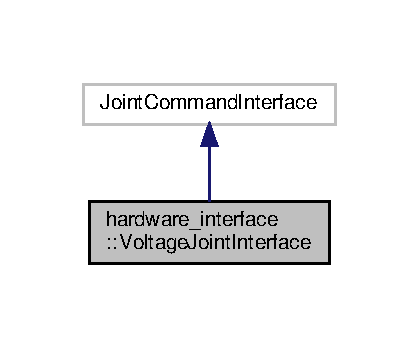
\includegraphics[width=201pt]{classhardware__interface_1_1_voltage_joint_interface__inherit__graph}
\end{center}
\end{figure}


Collaboration diagram for hardware\+\_\+interface\+:\+:Voltage\+Joint\+Interface\+:
\nopagebreak
\begin{figure}[H]
\begin{center}
\leavevmode
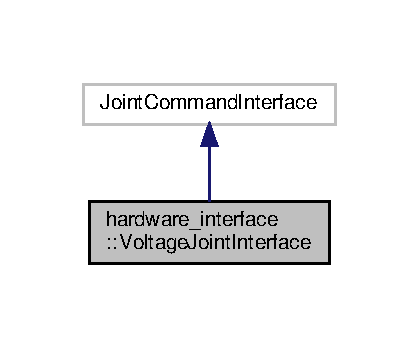
\includegraphics[width=201pt]{classhardware__interface_1_1_voltage_joint_interface__coll__graph}
\end{center}
\end{figure}


\subsection{Detailed Description}
Joint\+Command\+Interface for commanding voltage-\/based joints. 

The documentation for this class was generated from the following file\+:\begin{DoxyCompactItemize}
\item 
uwrt\+\_\+arm\+\_\+hw/include/uwrt\+\_\+arm\+\_\+hw/\hyperlink{voltage__joint__interface_8h}{voltage\+\_\+joint\+\_\+interface.\+h}\end{DoxyCompactItemize}

\chapter{File Documentation}
\hypertarget{delta__joint__publisher_8h}{}\section{uwrt\+\_\+arm\+\_\+control/include/uwrt\+\_\+arm\+\_\+control/delta\+\_\+joint\+\_\+publisher.h File Reference}
\label{delta__joint__publisher_8h}\index{uwrt\+\_\+arm\+\_\+control/include/uwrt\+\_\+arm\+\_\+control/delta\+\_\+joint\+\_\+publisher.\+h@{uwrt\+\_\+arm\+\_\+control/include/uwrt\+\_\+arm\+\_\+control/delta\+\_\+joint\+\_\+publisher.\+h}}
{\ttfamily \#include \char`\"{}uwrt\+\_\+arm\+\_\+msgs/\+U\+W\+R\+T\+Arm\+Command.\+h\char`\"{}}\newline
{\ttfamily \#include $<$control\+\_\+msgs/\+Joint\+Jog.\+h$>$}\newline
{\ttfamily \#include $<$ros/ros.\+h$>$}\newline
Include dependency graph for delta\+\_\+joint\+\_\+publisher.\+h\+:
\nopagebreak
\begin{figure}[H]
\begin{center}
\leavevmode
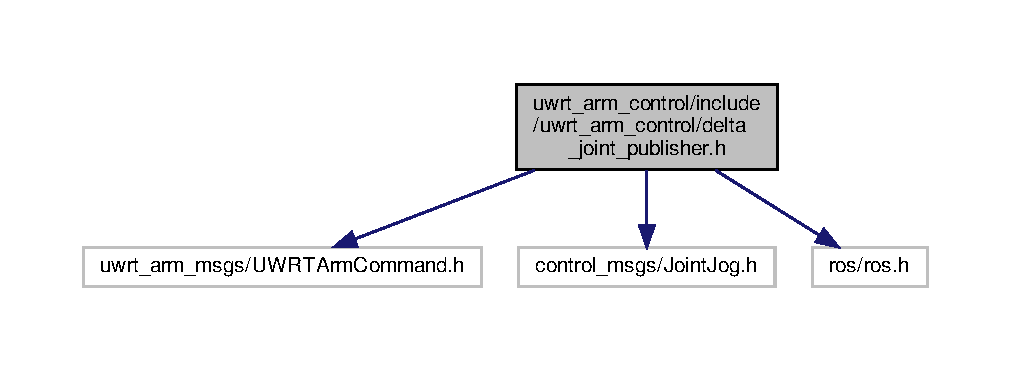
\includegraphics[width=350pt]{delta__joint__publisher_8h__incl}
\end{center}
\end{figure}
This graph shows which files directly or indirectly include this file\+:
\nopagebreak
\begin{figure}[H]
\begin{center}
\leavevmode
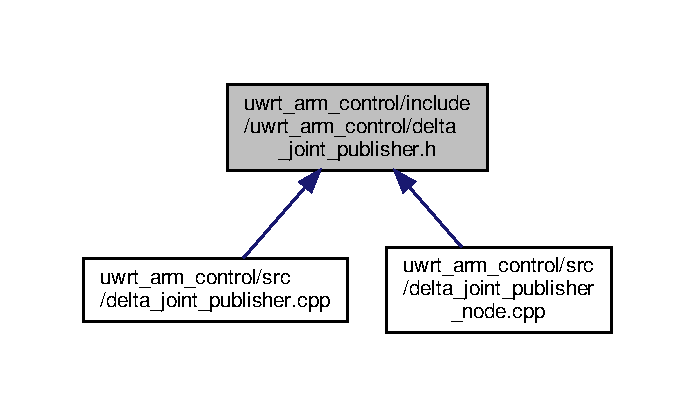
\includegraphics[width=334pt]{delta__joint__publisher_8h__dep__incl}
\end{center}
\end{figure}
\subsection*{Classes}
\begin{DoxyCompactItemize}
\item 
class \hyperlink{classuwrt_1_1arm_1_1_delta_joint_publisher}{uwrt\+::arm\+::\+Delta\+Joint\+Publisher}
\end{DoxyCompactItemize}
\subsection*{Namespaces}
\begin{DoxyCompactItemize}
\item 
 \hyperlink{namespaceuwrt}{uwrt}
\item 
 \hyperlink{namespaceuwrt_1_1arm}{uwrt\+::arm}
\end{DoxyCompactItemize}

\hypertarget{delta__joint__publisher_8cpp}{}\section{uwrt\+\_\+arm\+\_\+control/src/delta\+\_\+joint\+\_\+publisher.cpp File Reference}
\label{delta__joint__publisher_8cpp}\index{uwrt\+\_\+arm\+\_\+control/src/delta\+\_\+joint\+\_\+publisher.\+cpp@{uwrt\+\_\+arm\+\_\+control/src/delta\+\_\+joint\+\_\+publisher.\+cpp}}
{\ttfamily \#include \char`\"{}uwrt\+\_\+arm\+\_\+control/delta\+\_\+joint\+\_\+publisher.\+h\char`\"{}}\newline
{\ttfamily \#include \char`\"{}uwrt\+\_\+arm\+\_\+msgs/\+U\+W\+R\+T\+Arm\+Command.\+h\char`\"{}}\newline
{\ttfamily \#include $<$control\+\_\+msgs/\+Joint\+Jog.\+h$>$}\newline
{\ttfamily \#include $<$ros/ros.\+h$>$}\newline
Include dependency graph for delta\+\_\+joint\+\_\+publisher.\+cpp\+:
\nopagebreak
\begin{figure}[H]
\begin{center}
\leavevmode
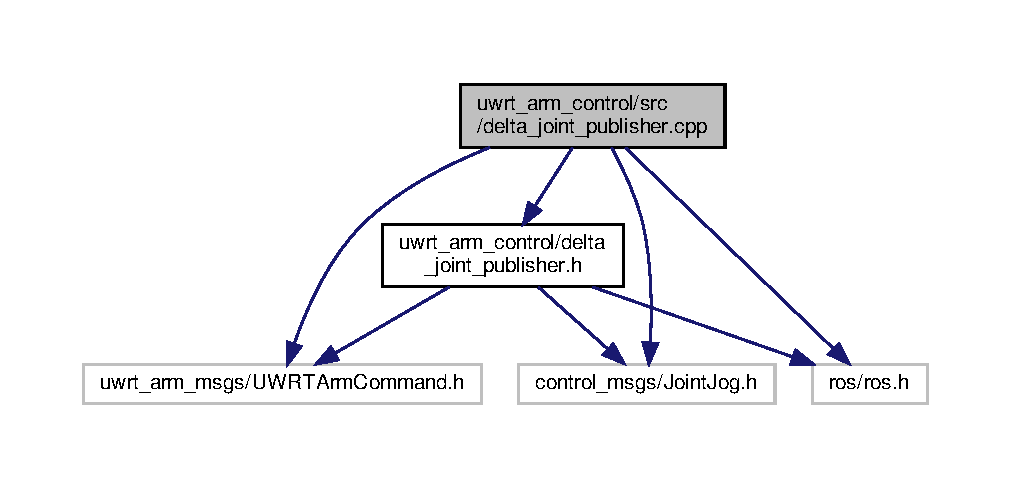
\includegraphics[width=350pt]{delta__joint__publisher_8cpp__incl}
\end{center}
\end{figure}
\subsection*{Namespaces}
\begin{DoxyCompactItemize}
\item 
 \hyperlink{namespaceuwrt}{uwrt}
\item 
 \hyperlink{namespaceuwrt_1_1arm}{uwrt\+::arm}
\end{DoxyCompactItemize}

\hypertarget{delta__joint__publisher__node_8cpp}{}\section{uwrt\+\_\+arm\+\_\+control/src/delta\+\_\+joint\+\_\+publisher\+\_\+node.cpp File Reference}
\label{delta__joint__publisher__node_8cpp}\index{uwrt\+\_\+arm\+\_\+control/src/delta\+\_\+joint\+\_\+publisher\+\_\+node.\+cpp@{uwrt\+\_\+arm\+\_\+control/src/delta\+\_\+joint\+\_\+publisher\+\_\+node.\+cpp}}
{\ttfamily \#include \char`\"{}uwrt\+\_\+arm\+\_\+control/delta\+\_\+joint\+\_\+publisher.\+h\char`\"{}}\newline
{\ttfamily \#include $<$ros/ros.\+h$>$}\newline
Include dependency graph for delta\+\_\+joint\+\_\+publisher\+\_\+node.\+cpp\+:
\nopagebreak
\begin{figure}[H]
\begin{center}
\leavevmode
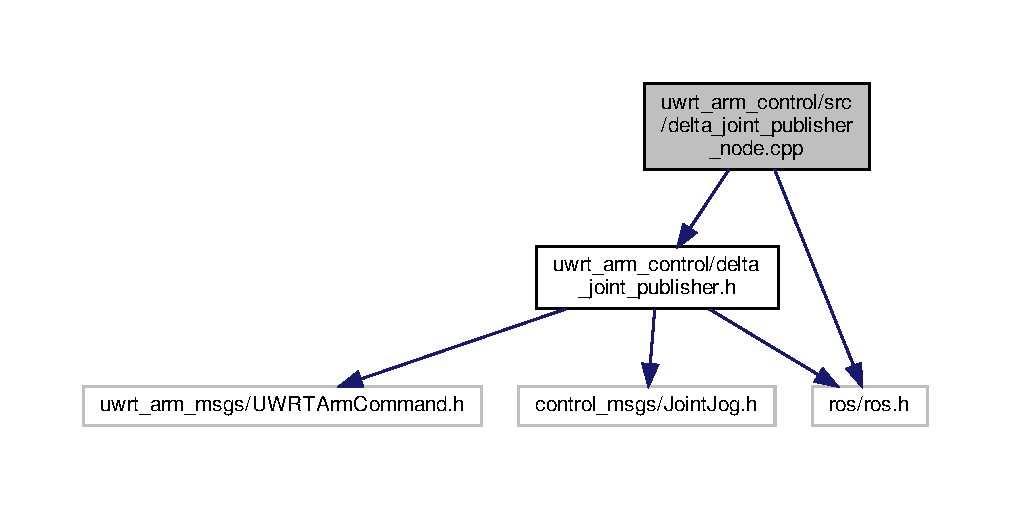
\includegraphics[width=350pt]{delta__joint__publisher__node_8cpp__incl}
\end{center}
\end{figure}
\subsection*{Functions}
\begin{DoxyCompactItemize}
\item 
int \hyperlink{delta__joint__publisher__node_8cpp_a3c04138a5bfe5d72780bb7e82a18e627}{main} (int argc, char $\ast$$\ast$argv)
\end{DoxyCompactItemize}


\subsection{Function Documentation}
\mbox{\Hypertarget{delta__joint__publisher__node_8cpp_a3c04138a5bfe5d72780bb7e82a18e627}\label{delta__joint__publisher__node_8cpp_a3c04138a5bfe5d72780bb7e82a18e627}} 
\index{delta\+\_\+joint\+\_\+publisher\+\_\+node.\+cpp@{delta\+\_\+joint\+\_\+publisher\+\_\+node.\+cpp}!main@{main}}
\index{main@{main}!delta\+\_\+joint\+\_\+publisher\+\_\+node.\+cpp@{delta\+\_\+joint\+\_\+publisher\+\_\+node.\+cpp}}
\subsubsection{\texorpdfstring{main()}{main()}}
{\footnotesize\ttfamily int main (\begin{DoxyParamCaption}\item[{int}]{argc,  }\item[{char $\ast$$\ast$}]{argv }\end{DoxyParamCaption})}

Copyright (c) 2020 Somesh Daga \href{mailto:s2daga@uwaterloo.ca}{\tt s2daga@uwaterloo.\+ca}

Permission is hereby granted, free of charge, to any person obtaining a copy of this software and associated documentation files (the \char`\"{}\+Software\char`\"{}), to deal in the Software without restriction, including without limitation the rights to use, copy, modify, merge, publish, distribute, sublicense, and/or sell copies of the Software, and to permit persons to whom the Software is furnished to do so, subject to the following conditions\+:

The above copyright notice and this permission notice shall be included in all copies or substantial portions of the Software.

T\+HE S\+O\+F\+T\+W\+A\+RE IS P\+R\+O\+V\+I\+D\+ED \char`\"{}\+A\+S I\+S\char`\"{}, W\+I\+T\+H\+O\+UT W\+A\+R\+R\+A\+N\+TY OF A\+NY K\+I\+ND, E\+X\+P\+R\+E\+SS OR I\+M\+P\+L\+I\+ED, I\+N\+C\+L\+U\+D\+I\+NG B\+UT N\+OT L\+I\+M\+I\+T\+ED TO T\+HE W\+A\+R\+R\+A\+N\+T\+I\+ES OF M\+E\+R\+C\+H\+A\+N\+T\+A\+B\+I\+L\+I\+TY, F\+I\+T\+N\+E\+SS F\+OR A P\+A\+R\+T\+I\+C\+U\+L\+AR P\+U\+R\+P\+O\+SE A\+ND N\+O\+N\+I\+N\+F\+R\+I\+N\+G\+E\+M\+E\+NT. IN NO E\+V\+E\+NT S\+H\+A\+LL T\+HE A\+U\+T\+H\+O\+RS OR C\+O\+P\+Y\+R\+I\+G\+HT H\+O\+L\+D\+E\+RS BE L\+I\+A\+B\+LE F\+OR A\+NY C\+L\+A\+IM, D\+A\+M\+A\+G\+ES OR O\+T\+H\+ER L\+I\+A\+B\+I\+L\+I\+TY, W\+H\+E\+T\+H\+ER IN AN A\+C\+T\+I\+ON OF C\+O\+N\+T\+R\+A\+CT, T\+O\+RT OR O\+T\+H\+E\+R\+W\+I\+SE, A\+R\+I\+S\+I\+NG F\+R\+OM, O\+UT OF OR IN C\+O\+N\+N\+E\+C\+T\+I\+ON W\+I\+TH T\+HE S\+O\+F\+T\+W\+A\+RE OR T\+HE U\+SE OR O\+T\+H\+ER D\+E\+A\+L\+I\+N\+GS IN T\+HE S\+O\+F\+T\+W\+A\+RE. 
\hypertarget{uwrt__arm__description_2_r_e_a_d_m_e_8md}{}\section{uwrt\+\_\+arm\+\_\+description/\+R\+E\+A\+D\+ME.md File Reference}
\label{uwrt__arm__description_2_r_e_a_d_m_e_8md}\index{uwrt\+\_\+arm\+\_\+description/\+R\+E\+A\+D\+M\+E.\+md@{uwrt\+\_\+arm\+\_\+description/\+R\+E\+A\+D\+M\+E.\+md}}

\hypertarget{uwrt__arm__hw_2_r_e_a_d_m_e_8md}{}\section{uwrt\+\_\+arm\+\_\+hw/\+R\+E\+A\+D\+ME.md File Reference}
\label{uwrt__arm__hw_2_r_e_a_d_m_e_8md}\index{uwrt\+\_\+arm\+\_\+hw/\+R\+E\+A\+D\+M\+E.\+md@{uwrt\+\_\+arm\+\_\+hw/\+R\+E\+A\+D\+M\+E.\+md}}

\hypertarget{arm__control__loop_8h}{}\section{uwrt\+\_\+arm\+\_\+hw/include/uwrt\+\_\+arm\+\_\+hw/arm\+\_\+control\+\_\+loop.h File Reference}
\label{arm__control__loop_8h}\index{uwrt\+\_\+arm\+\_\+hw/include/uwrt\+\_\+arm\+\_\+hw/arm\+\_\+control\+\_\+loop.\+h@{uwrt\+\_\+arm\+\_\+hw/include/uwrt\+\_\+arm\+\_\+hw/arm\+\_\+control\+\_\+loop.\+h}}
{\ttfamily \#include \char`\"{}uwrt\+\_\+arm\+\_\+hw/arm\+\_\+hw.\+h\char`\"{}}\newline
{\ttfamily \#include $<$controller\+\_\+manager/controller\+\_\+manager.\+h$>$}\newline
{\ttfamily \#include $<$ros/ros.\+h$>$}\newline
{\ttfamily \#include $<$string$>$}\newline
Include dependency graph for arm\+\_\+control\+\_\+loop.\+h\+:
\nopagebreak
\begin{figure}[H]
\begin{center}
\leavevmode
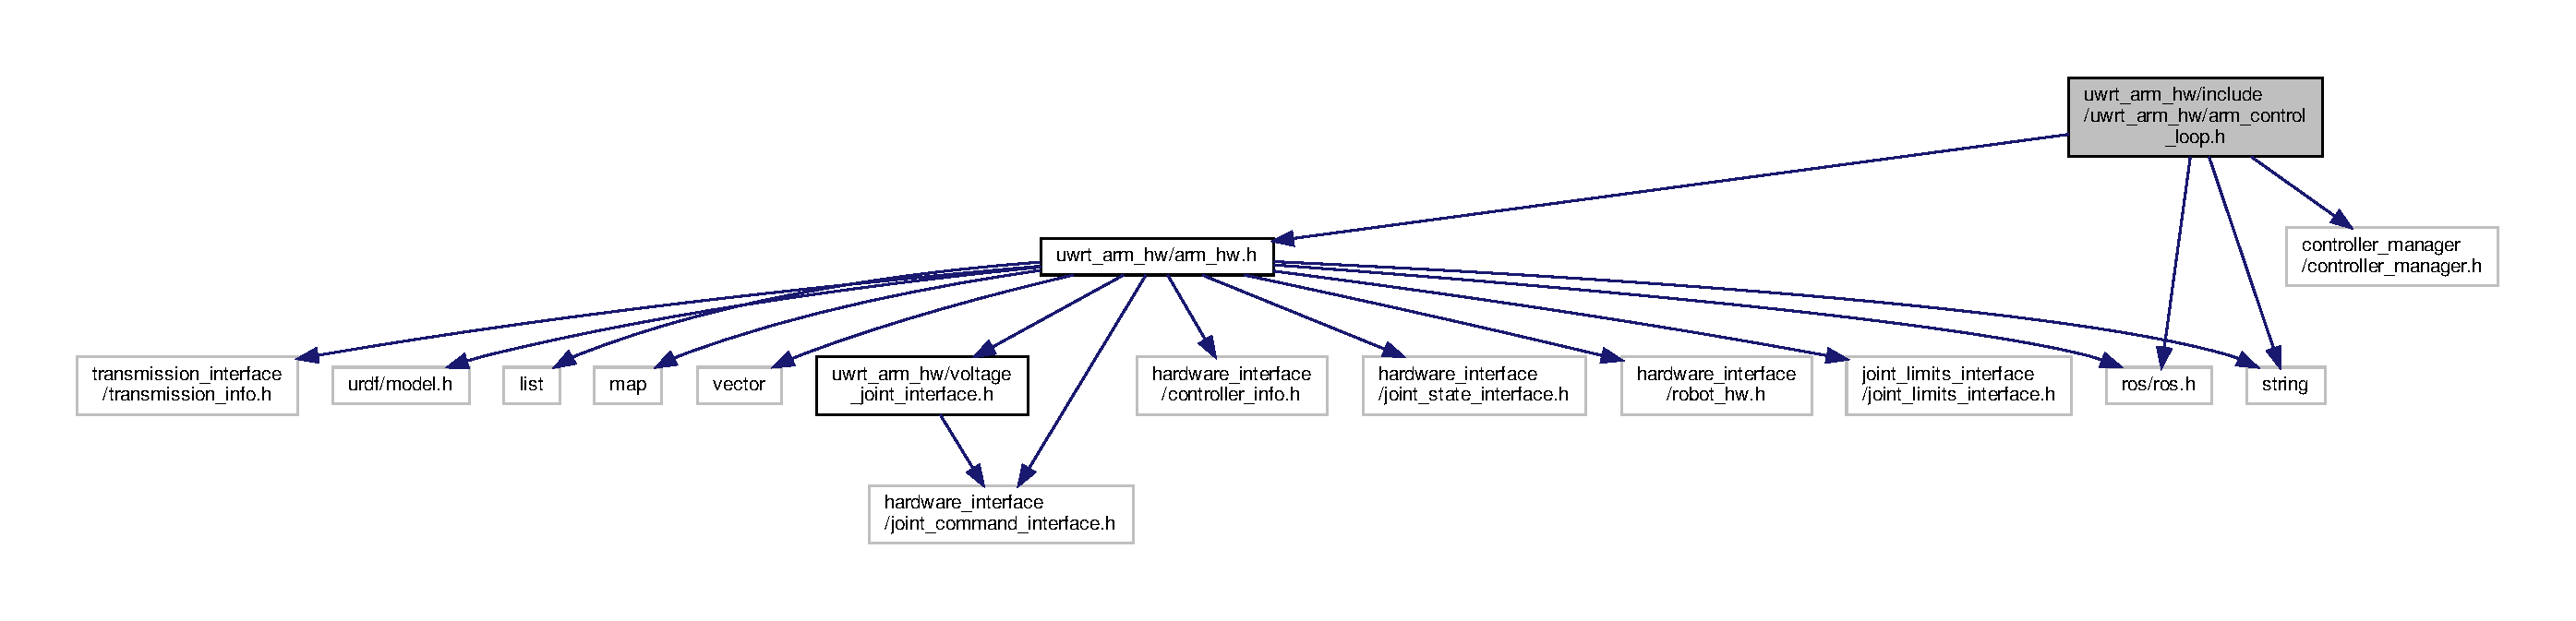
\includegraphics[width=350pt]{arm__control__loop_8h__incl}
\end{center}
\end{figure}
This graph shows which files directly or indirectly include this file\+:
\nopagebreak
\begin{figure}[H]
\begin{center}
\leavevmode
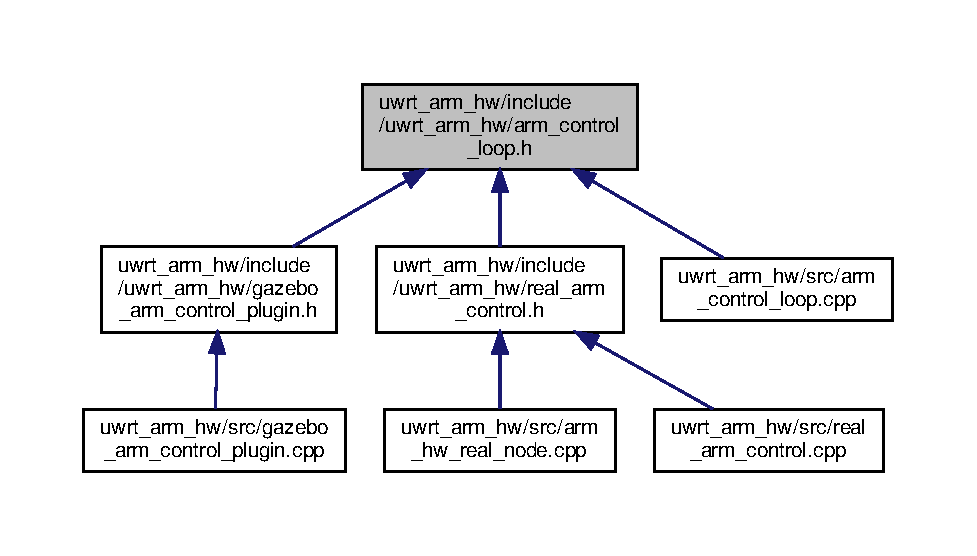
\includegraphics[width=350pt]{arm__control__loop_8h__dep__incl}
\end{center}
\end{figure}
\subsection*{Classes}
\begin{DoxyCompactItemize}
\item 
class \hyperlink{classuwrt_1_1arm_1_1_arm_control_loop}{uwrt\+::arm\+::\+Arm\+Control\+Loop}
\end{DoxyCompactItemize}
\subsection*{Namespaces}
\begin{DoxyCompactItemize}
\item 
 \hyperlink{namespaceuwrt}{uwrt}
\item 
 \hyperlink{namespaceuwrt_1_1arm}{uwrt\+::arm}
\end{DoxyCompactItemize}

\hypertarget{arm__hw_8h}{}\section{uwrt\+\_\+arm\+\_\+hw/include/uwrt\+\_\+arm\+\_\+hw/arm\+\_\+hw.h File Reference}
\label{arm__hw_8h}\index{uwrt\+\_\+arm\+\_\+hw/include/uwrt\+\_\+arm\+\_\+hw/arm\+\_\+hw.\+h@{uwrt\+\_\+arm\+\_\+hw/include/uwrt\+\_\+arm\+\_\+hw/arm\+\_\+hw.\+h}}
{\ttfamily \#include \char`\"{}uwrt\+\_\+arm\+\_\+hw/voltage\+\_\+joint\+\_\+interface.\+h\char`\"{}}\newline
{\ttfamily \#include $<$hardware\+\_\+interface/controller\+\_\+info.\+h$>$}\newline
{\ttfamily \#include $<$hardware\+\_\+interface/joint\+\_\+command\+\_\+interface.\+h$>$}\newline
{\ttfamily \#include $<$hardware\+\_\+interface/joint\+\_\+state\+\_\+interface.\+h$>$}\newline
{\ttfamily \#include $<$hardware\+\_\+interface/robot\+\_\+hw.\+h$>$}\newline
{\ttfamily \#include $<$joint\+\_\+limits\+\_\+interface/joint\+\_\+limits\+\_\+interface.\+h$>$}\newline
{\ttfamily \#include $<$ros/ros.\+h$>$}\newline
{\ttfamily \#include $<$transmission\+\_\+interface/transmission\+\_\+info.\+h$>$}\newline
{\ttfamily \#include $<$urdf/model.\+h$>$}\newline
{\ttfamily \#include $<$list$>$}\newline
{\ttfamily \#include $<$map$>$}\newline
{\ttfamily \#include $<$string$>$}\newline
{\ttfamily \#include $<$vector$>$}\newline
Include dependency graph for arm\+\_\+hw.\+h\+:
\nopagebreak
\begin{figure}[H]
\begin{center}
\leavevmode
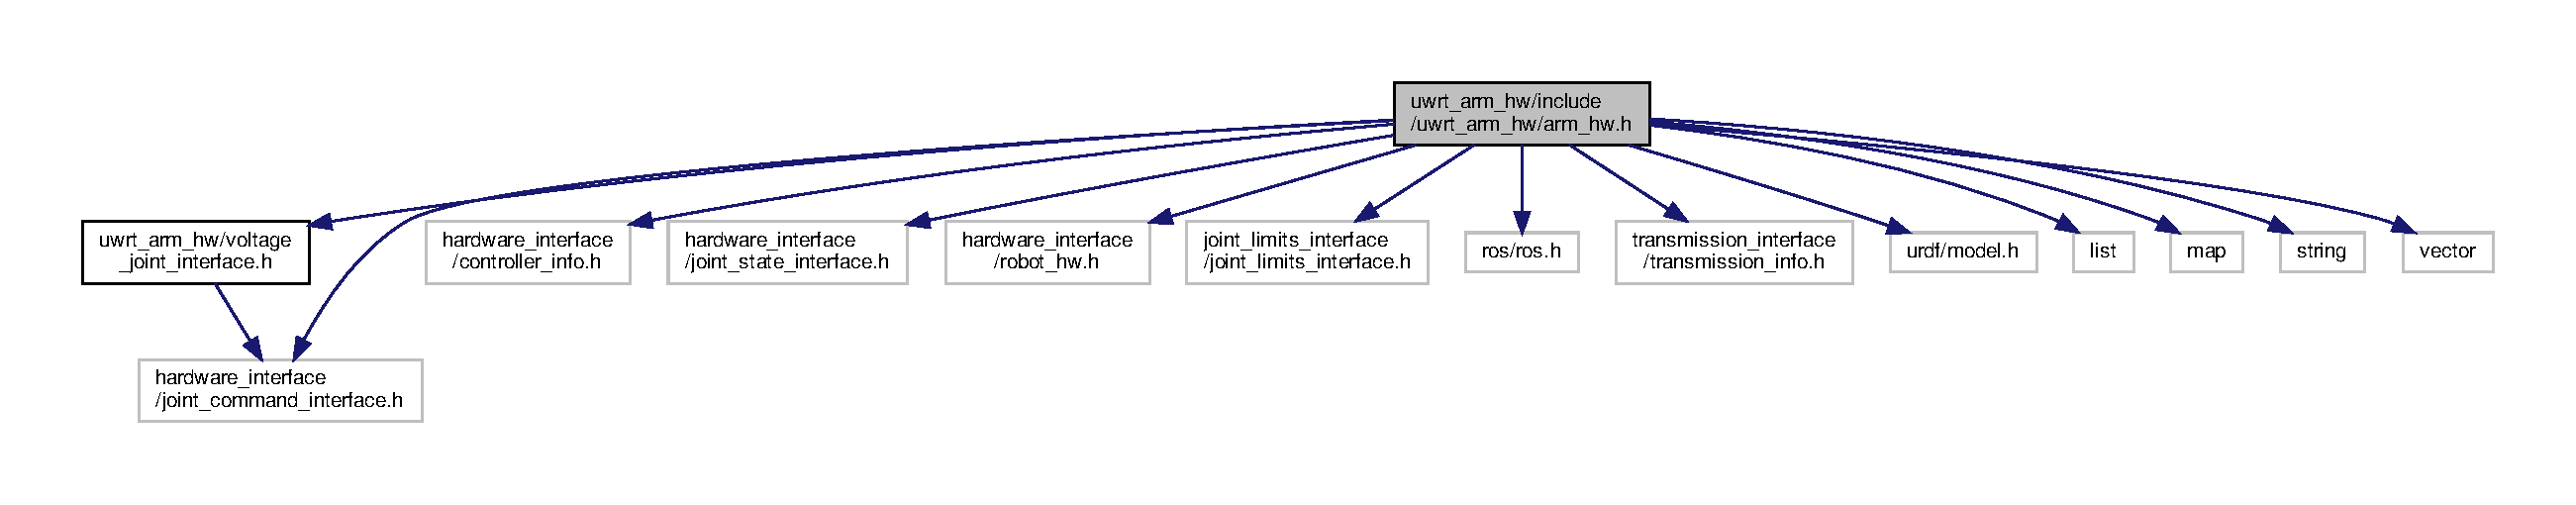
\includegraphics[width=350pt]{arm__hw_8h__incl}
\end{center}
\end{figure}
This graph shows which files directly or indirectly include this file\+:
\nopagebreak
\begin{figure}[H]
\begin{center}
\leavevmode
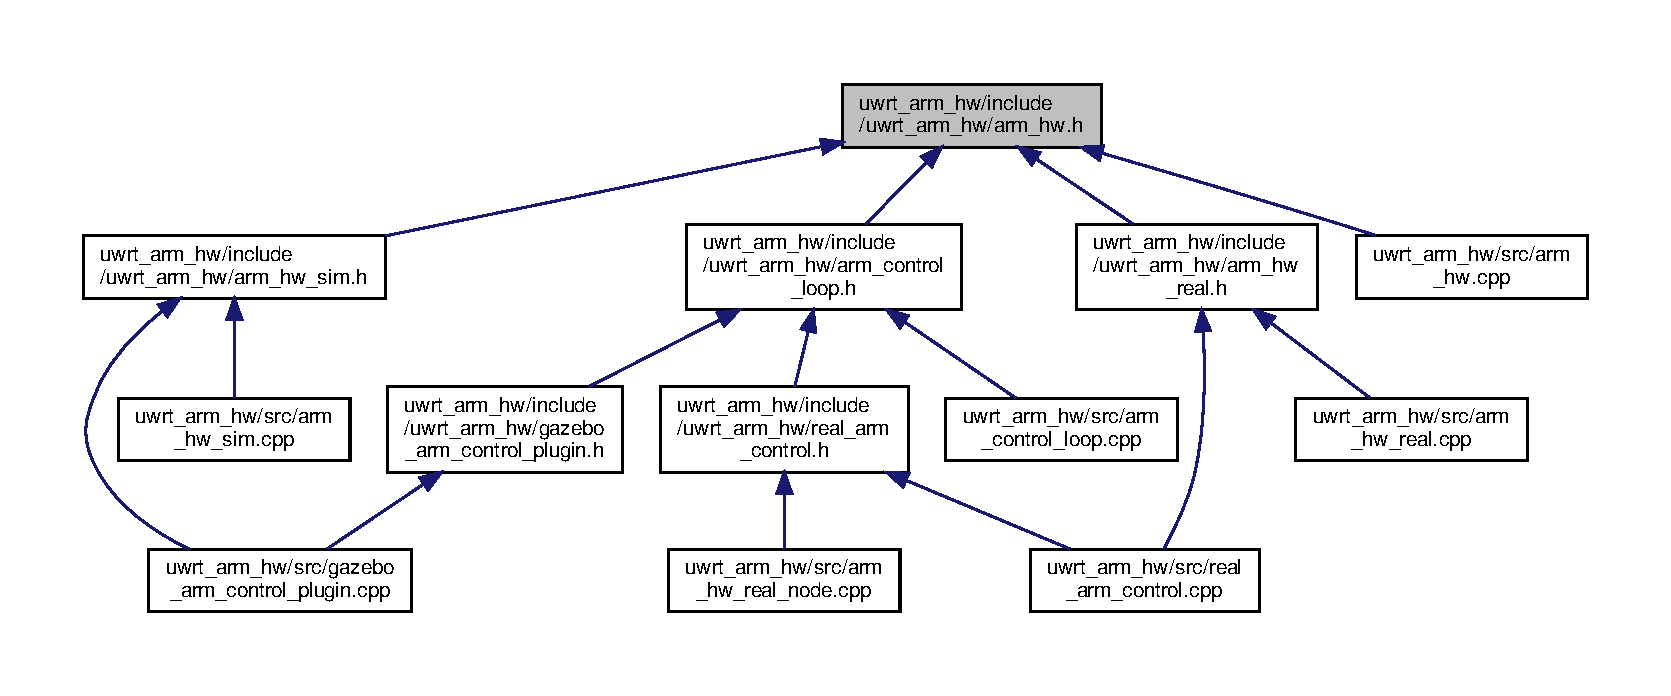
\includegraphics[width=350pt]{arm__hw_8h__dep__incl}
\end{center}
\end{figure}
\subsection*{Classes}
\begin{DoxyCompactItemize}
\item 
class \hyperlink{classuwrt_1_1arm_1_1_arm_h_w}{uwrt\+::arm\+::\+Arm\+HW}
\end{DoxyCompactItemize}
\subsection*{Namespaces}
\begin{DoxyCompactItemize}
\item 
 \hyperlink{namespaceuwrt}{uwrt}
\item 
 \hyperlink{namespaceuwrt_1_1arm}{uwrt\+::arm}
\end{DoxyCompactItemize}

\hypertarget{arm__hw__real_8h}{}\section{uwrt\+\_\+arm\+\_\+hw/include/uwrt\+\_\+arm\+\_\+hw/arm\+\_\+hw\+\_\+real.h File Reference}
\label{arm__hw__real_8h}\index{uwrt\+\_\+arm\+\_\+hw/include/uwrt\+\_\+arm\+\_\+hw/arm\+\_\+hw\+\_\+real.\+h@{uwrt\+\_\+arm\+\_\+hw/include/uwrt\+\_\+arm\+\_\+hw/arm\+\_\+hw\+\_\+real.\+h}}
{\ttfamily \#include \char`\"{}uwrt\+\_\+arm\+\_\+hw/arm\+\_\+hw.\+h\char`\"{}}\newline
{\ttfamily \#include $<$ros/ros.\+h$>$}\newline
{\ttfamily \#include $<$linux/can.\+h$>$}\newline
{\ttfamily \#include $<$net/if.\+h$>$}\newline
{\ttfamily \#include $<$string$>$}\newline
Include dependency graph for arm\+\_\+hw\+\_\+real.\+h\+:
\nopagebreak
\begin{figure}[H]
\begin{center}
\leavevmode
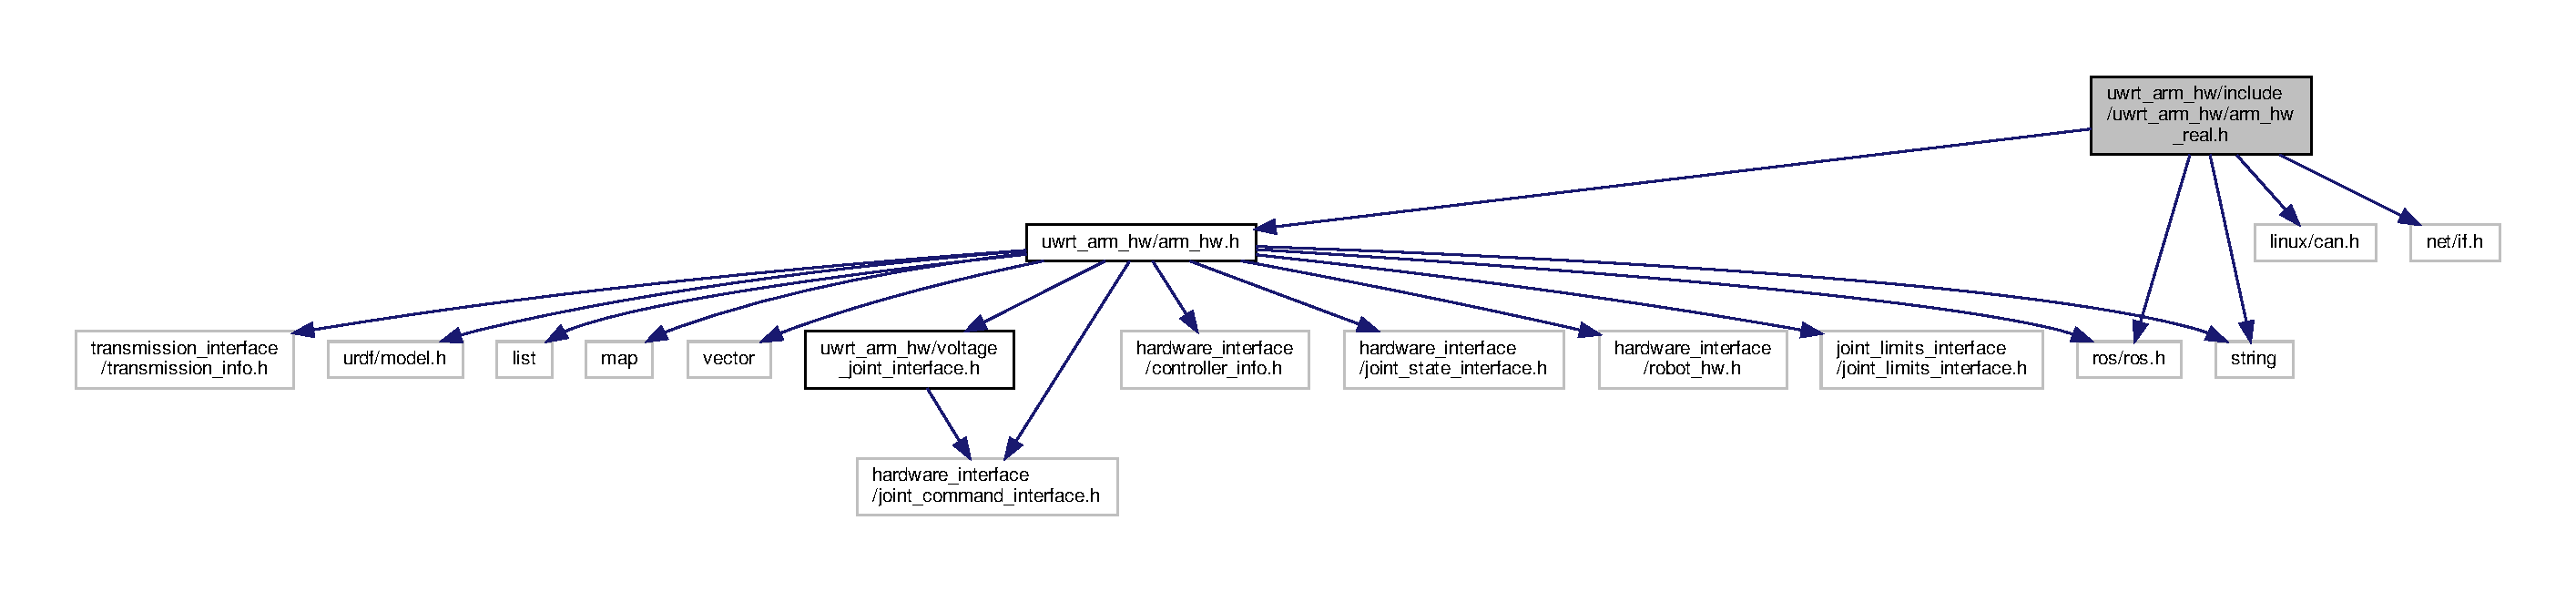
\includegraphics[width=350pt]{arm__hw__real_8h__incl}
\end{center}
\end{figure}
This graph shows which files directly or indirectly include this file\+:
\nopagebreak
\begin{figure}[H]
\begin{center}
\leavevmode
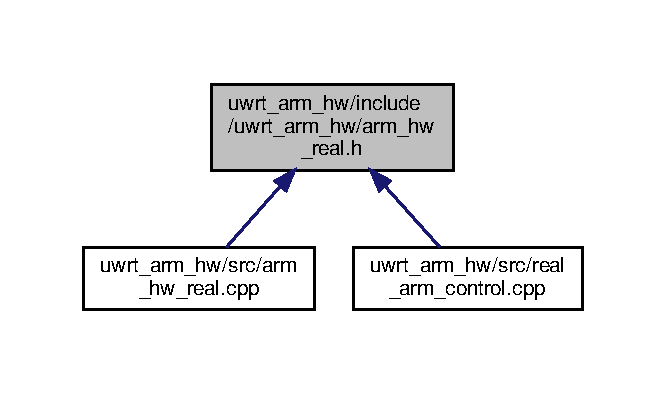
\includegraphics[width=320pt]{arm__hw__real_8h__dep__incl}
\end{center}
\end{figure}
\subsection*{Classes}
\begin{DoxyCompactItemize}
\item 
class \hyperlink{classuwrt_1_1arm_1_1_arm_h_w_real}{uwrt\+::arm\+::\+Arm\+H\+W\+Real}
\end{DoxyCompactItemize}
\subsection*{Namespaces}
\begin{DoxyCompactItemize}
\item 
 \hyperlink{namespaceuwrt}{uwrt}
\item 
 \hyperlink{namespaceuwrt_1_1arm}{uwrt\+::arm}
\end{DoxyCompactItemize}

\hypertarget{arm__hw__sim_8h}{}\section{uwrt\+\_\+arm\+\_\+hw/include/uwrt\+\_\+arm\+\_\+hw/arm\+\_\+hw\+\_\+sim.h File Reference}
\label{arm__hw__sim_8h}\index{uwrt\+\_\+arm\+\_\+hw/include/uwrt\+\_\+arm\+\_\+hw/arm\+\_\+hw\+\_\+sim.\+h@{uwrt\+\_\+arm\+\_\+hw/include/uwrt\+\_\+arm\+\_\+hw/arm\+\_\+hw\+\_\+sim.\+h}}
{\ttfamily \#include \char`\"{}uwrt\+\_\+arm\+\_\+hw/arm\+\_\+hw.\+h\char`\"{}}\newline
{\ttfamily \#include $<$gazebo/physics/physics.\+hh$>$}\newline
{\ttfamily \#include $<$ros/ros.\+h$>$}\newline
{\ttfamily \#include $<$boost/shared\+\_\+ptr.\+hpp$>$}\newline
{\ttfamily \#include $<$string$>$}\newline
{\ttfamily \#include $<$vector$>$}\newline
Include dependency graph for arm\+\_\+hw\+\_\+sim.\+h\+:
\nopagebreak
\begin{figure}[H]
\begin{center}
\leavevmode
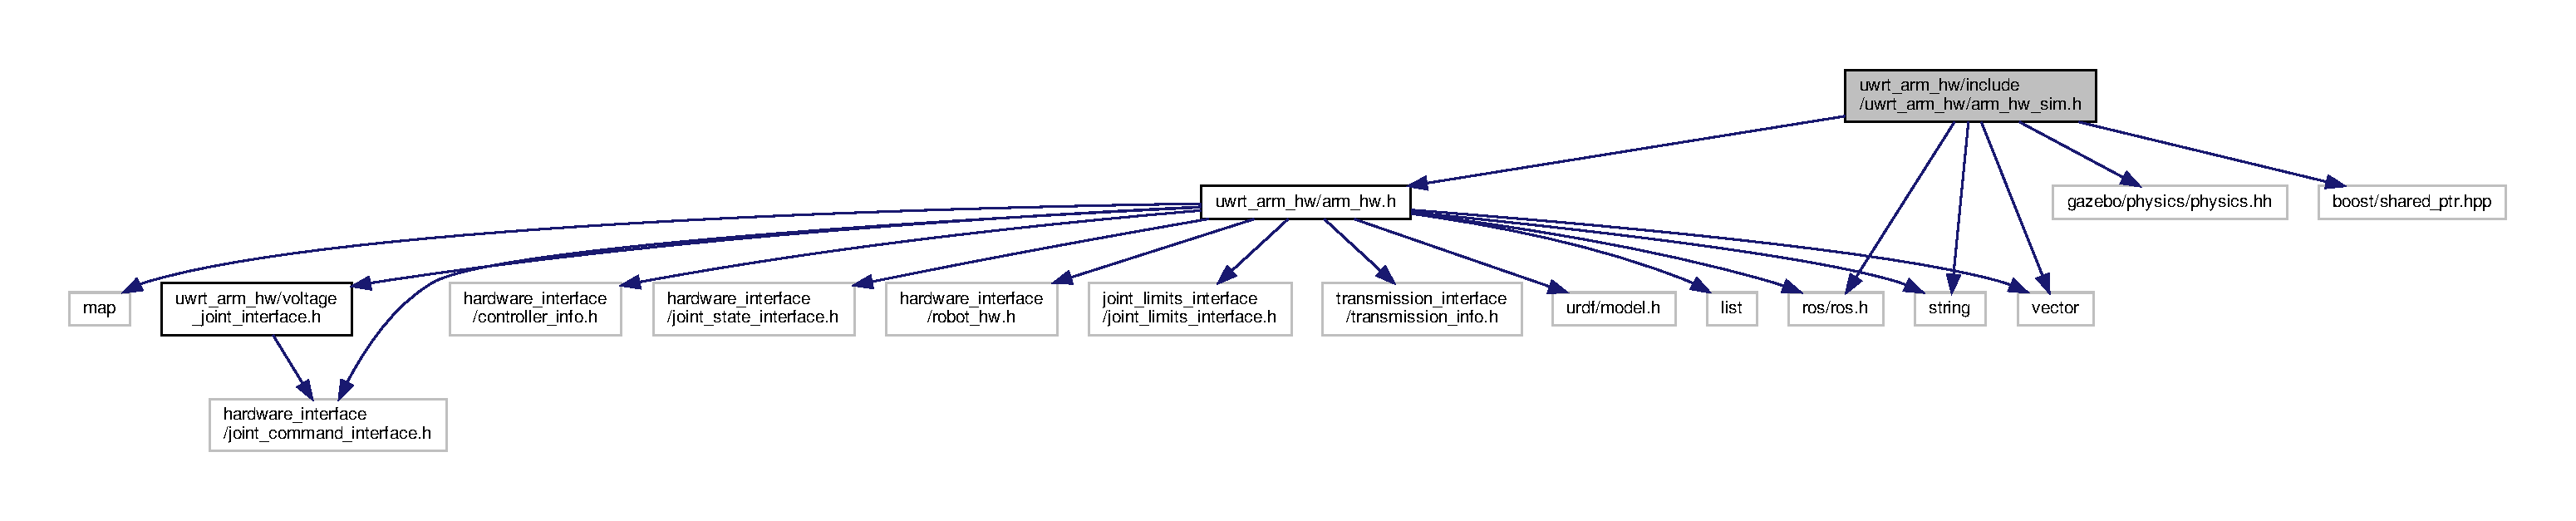
\includegraphics[width=350pt]{arm__hw__sim_8h__incl}
\end{center}
\end{figure}
This graph shows which files directly or indirectly include this file\+:
\nopagebreak
\begin{figure}[H]
\begin{center}
\leavevmode
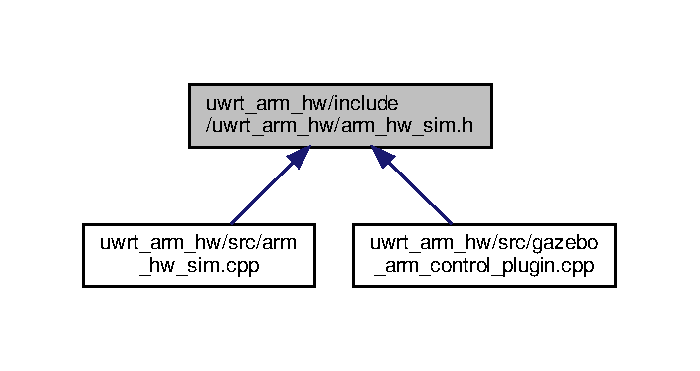
\includegraphics[width=336pt]{arm__hw__sim_8h__dep__incl}
\end{center}
\end{figure}
\subsection*{Classes}
\begin{DoxyCompactItemize}
\item 
class \hyperlink{classuwrt_1_1arm_1_1_arm_h_w_sim}{uwrt\+::arm\+::\+Arm\+H\+W\+Sim}
\end{DoxyCompactItemize}
\subsection*{Namespaces}
\begin{DoxyCompactItemize}
\item 
 \hyperlink{namespaceuwrt}{uwrt}
\item 
 \hyperlink{namespaceuwrt_1_1arm}{uwrt\+::arm}
\end{DoxyCompactItemize}
\subsection*{Typedefs}
\begin{DoxyCompactItemize}
\item 
typedef boost\+::shared\+\_\+ptr$<$ Arm\+H\+W\+Sim $>$ \hyperlink{namespaceuwrt_1_1arm_a74b3a52f0f9eae5e40d20a1a07334eb8}{uwrt\+::arm\+::\+Arm\+H\+W\+Sim\+Ptr}
\end{DoxyCompactItemize}

\hypertarget{can__config_8h}{}\section{uwrt\+\_\+arm\+\_\+hw/include/uwrt\+\_\+arm\+\_\+hw/can\+\_\+config.h File Reference}
\label{can__config_8h}\index{uwrt\+\_\+arm\+\_\+hw/include/uwrt\+\_\+arm\+\_\+hw/can\+\_\+config.\+h@{uwrt\+\_\+arm\+\_\+hw/include/uwrt\+\_\+arm\+\_\+hw/can\+\_\+config.\+h}}
{\ttfamily \#include $<$linux/can.\+h$>$}\newline
Include dependency graph for can\+\_\+config.\+h\+:
\nopagebreak
\begin{figure}[H]
\begin{center}
\leavevmode
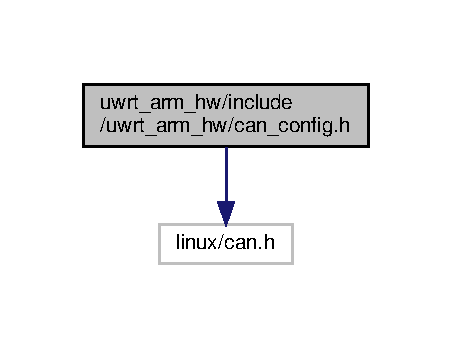
\includegraphics[width=217pt]{can__config_8h__incl}
\end{center}
\end{figure}
This graph shows which files directly or indirectly include this file\+:
\nopagebreak
\begin{figure}[H]
\begin{center}
\leavevmode
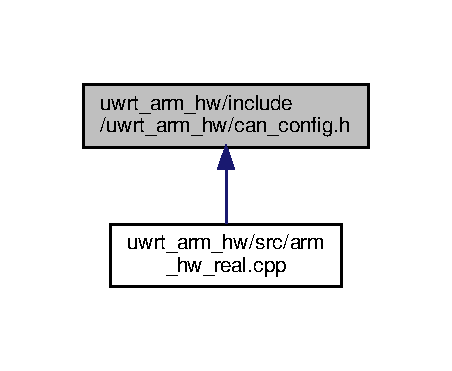
\includegraphics[width=217pt]{can__config_8h__dep__incl}
\end{center}
\end{figure}
\subsection*{Classes}
\begin{DoxyCompactItemize}
\item 
struct \hyperlink{structuwrt_1_1arm_1_1can__id_1_1_get}{uwrt\+::arm\+::can\+\_\+id\+::\+Get}
\item 
struct \hyperlink{structuwrt_1_1arm_1_1can__id_1_1_set}{uwrt\+::arm\+::can\+\_\+id\+::\+Set}
\item 
struct \hyperlink{structuwrt_1_1arm_1_1can__id_1_1_calibrate}{uwrt\+::arm\+::can\+\_\+id\+::\+Calibrate}
\end{DoxyCompactItemize}
\subsection*{Namespaces}
\begin{DoxyCompactItemize}
\item 
 \hyperlink{namespaceuwrt}{uwrt}
\item 
 \hyperlink{namespaceuwrt_1_1arm}{uwrt\+::arm}
\item 
 \hyperlink{namespaceuwrt_1_1arm_1_1can__id}{uwrt\+::arm\+::can\+\_\+id}
\end{DoxyCompactItemize}
\subsection*{Variables}
\begin{DoxyCompactItemize}
\item 
const uint8\+\_\+t \hyperlink{namespaceuwrt_1_1arm_ad353395d3b0d46797e243b550226f066}{uwrt\+::arm\+::\+C\+A\+N\+\_\+\+F\+R\+A\+M\+E\+\_\+\+S\+I\+Z\+E\+\_\+\+B\+Y\+T\+E\+S\+\_\+} = 8
\begin{DoxyCompactList}\small\item\em Maximum number of bytes for data field of the C\+AN frame. \end{DoxyCompactList}\end{DoxyCompactItemize}

\hypertarget{gazebo__arm__control__plugin_8h}{}\section{uwrt\+\_\+arm\+\_\+hw/include/uwrt\+\_\+arm\+\_\+hw/gazebo\+\_\+arm\+\_\+control\+\_\+plugin.h File Reference}
\label{gazebo__arm__control__plugin_8h}\index{uwrt\+\_\+arm\+\_\+hw/include/uwrt\+\_\+arm\+\_\+hw/gazebo\+\_\+arm\+\_\+control\+\_\+plugin.\+h@{uwrt\+\_\+arm\+\_\+hw/include/uwrt\+\_\+arm\+\_\+hw/gazebo\+\_\+arm\+\_\+control\+\_\+plugin.\+h}}
{\ttfamily \#include \char`\"{}uwrt\+\_\+arm\+\_\+hw/arm\+\_\+control\+\_\+loop.\+h\char`\"{}}\newline
{\ttfamily \#include $<$gazebo/common/common.\+hh$>$}\newline
{\ttfamily \#include $<$gazebo/gazebo.\+hh$>$}\newline
{\ttfamily \#include $<$gazebo/physics/physics.\+hh$>$}\newline
{\ttfamily \#include $<$ros/ros.\+h$>$}\newline
{\ttfamily \#include $<$string$>$}\newline
Include dependency graph for gazebo\+\_\+arm\+\_\+control\+\_\+plugin.\+h\+:
\nopagebreak
\begin{figure}[H]
\begin{center}
\leavevmode
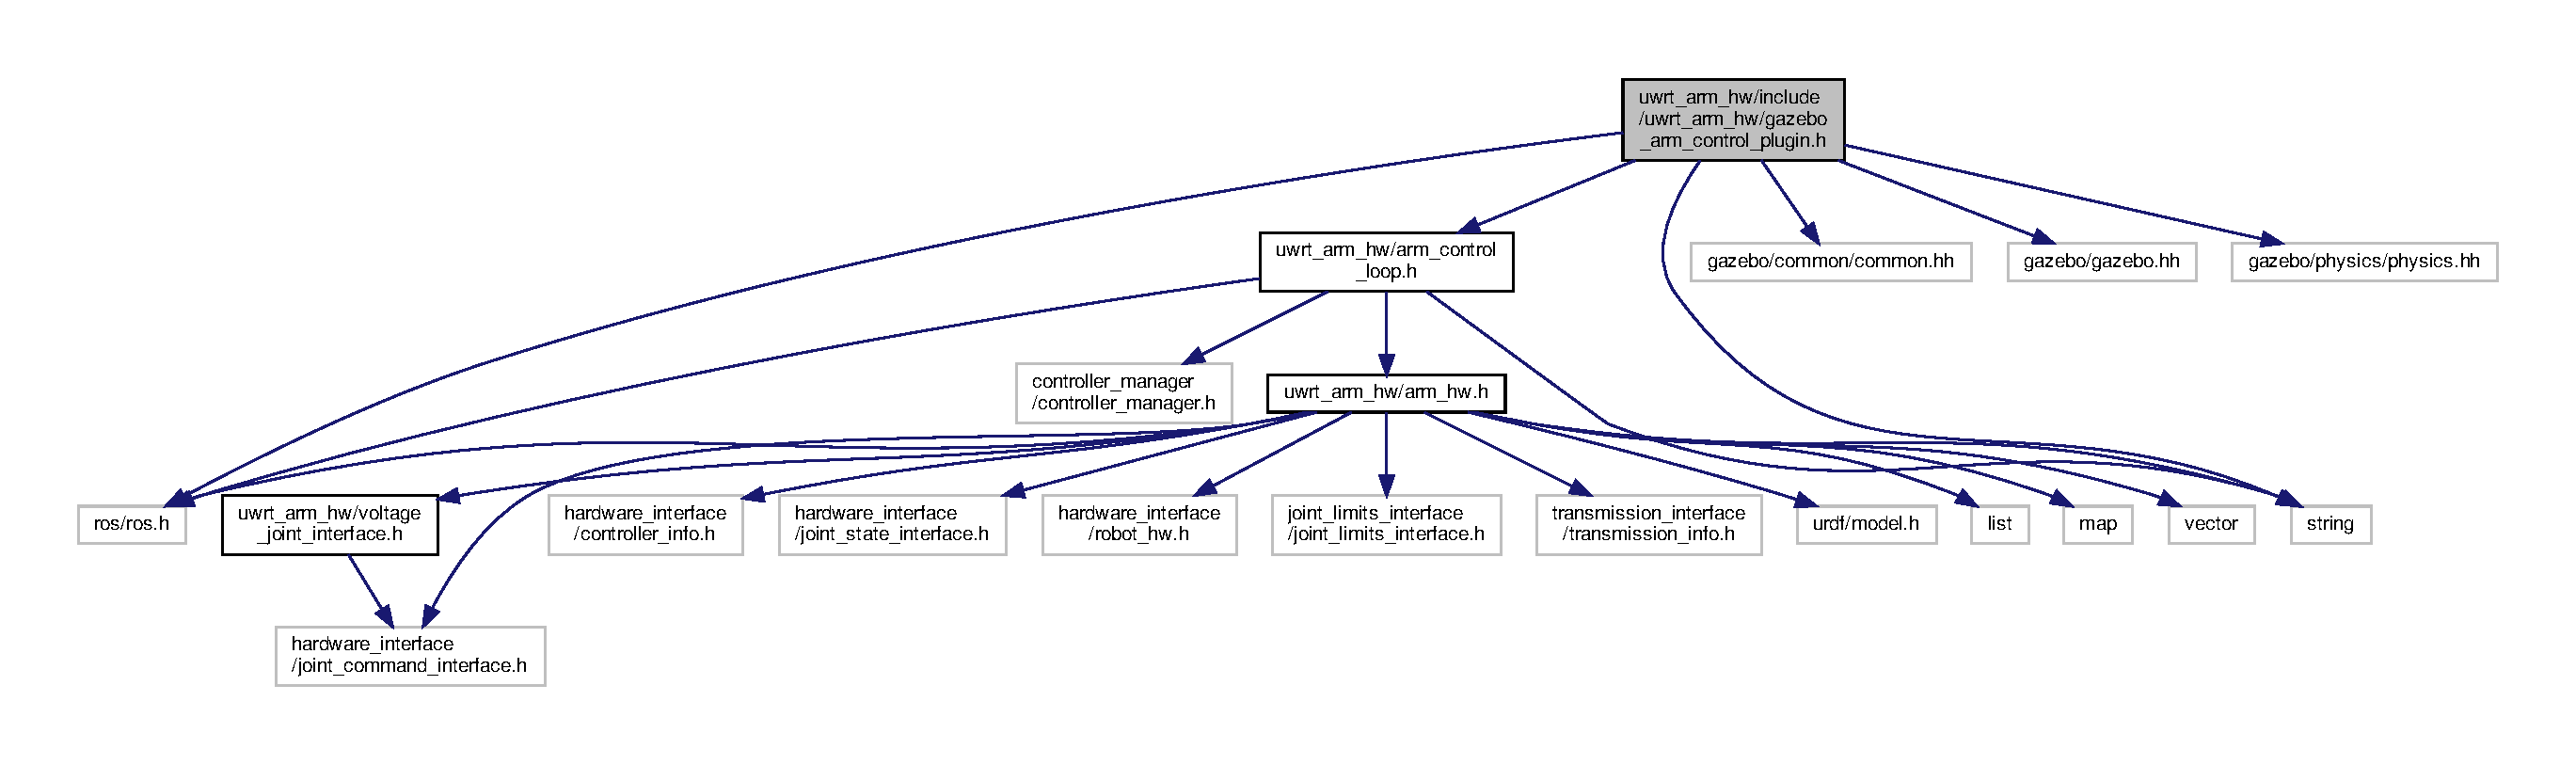
\includegraphics[width=350pt]{gazebo__arm__control__plugin_8h__incl}
\end{center}
\end{figure}
This graph shows which files directly or indirectly include this file\+:
\nopagebreak
\begin{figure}[H]
\begin{center}
\leavevmode
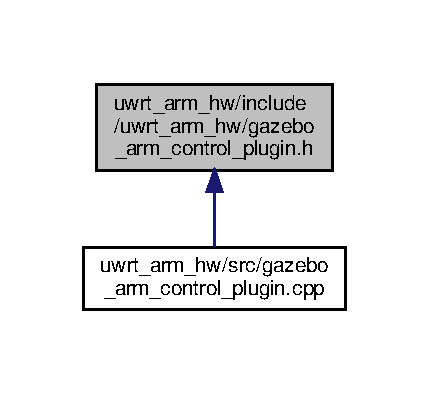
\includegraphics[width=206pt]{gazebo__arm__control__plugin_8h__dep__incl}
\end{center}
\end{figure}
\subsection*{Classes}
\begin{DoxyCompactItemize}
\item 
class \hyperlink{classuwrt_1_1arm_1_1_gazebo_arm_control_plugin}{uwrt\+::arm\+::\+Gazebo\+Arm\+Control\+Plugin}
\end{DoxyCompactItemize}
\subsection*{Namespaces}
\begin{DoxyCompactItemize}
\item 
 \hyperlink{namespaceuwrt}{uwrt}
\item 
 \hyperlink{namespaceuwrt_1_1arm}{uwrt\+::arm}
\end{DoxyCompactItemize}

\hypertarget{joint__group__voltage__controller_8h}{}\section{uwrt\+\_\+arm\+\_\+hw/include/uwrt\+\_\+arm\+\_\+hw/joint\+\_\+group\+\_\+voltage\+\_\+controller.h File Reference}
\label{joint__group__voltage__controller_8h}\index{uwrt\+\_\+arm\+\_\+hw/include/uwrt\+\_\+arm\+\_\+hw/joint\+\_\+group\+\_\+voltage\+\_\+controller.\+h@{uwrt\+\_\+arm\+\_\+hw/include/uwrt\+\_\+arm\+\_\+hw/joint\+\_\+group\+\_\+voltage\+\_\+controller.\+h}}
{\ttfamily \#include \char`\"{}uwrt\+\_\+arm\+\_\+hw/voltage\+\_\+joint\+\_\+interface.\+h\char`\"{}}\newline
{\ttfamily \#include $<$forward\+\_\+command\+\_\+controller/forward\+\_\+joint\+\_\+group\+\_\+command\+\_\+controller.\+h$>$}\newline
Include dependency graph for joint\+\_\+group\+\_\+voltage\+\_\+controller.\+h\+:
\nopagebreak
\begin{figure}[H]
\begin{center}
\leavevmode
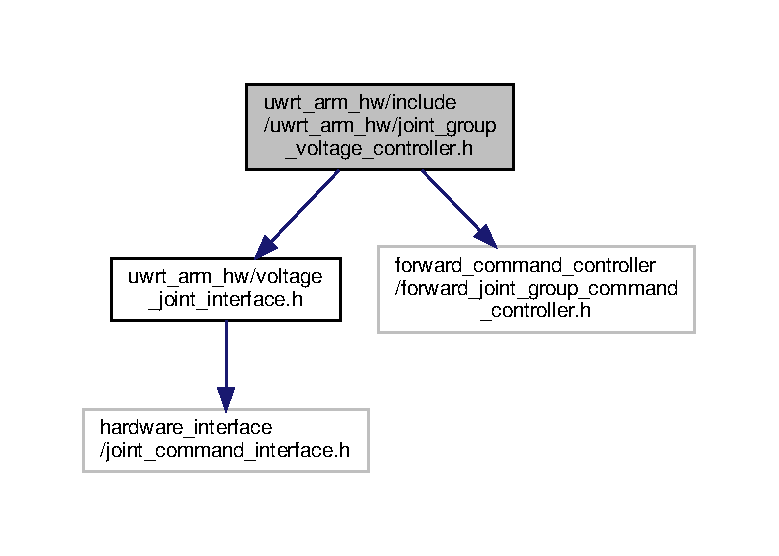
\includegraphics[width=350pt]{joint__group__voltage__controller_8h__incl}
\end{center}
\end{figure}
This graph shows which files directly or indirectly include this file\+:
\nopagebreak
\begin{figure}[H]
\begin{center}
\leavevmode
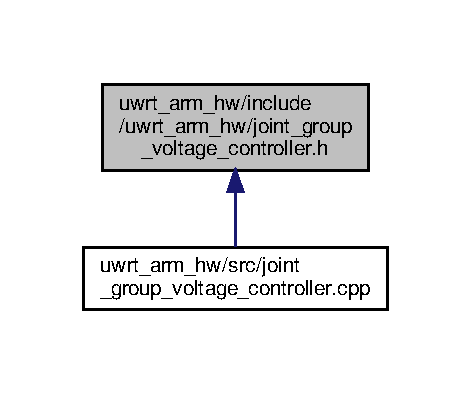
\includegraphics[width=226pt]{joint__group__voltage__controller_8h__dep__incl}
\end{center}
\end{figure}
\subsection*{Namespaces}
\begin{DoxyCompactItemize}
\item 
 \hyperlink{namespacevoltage__controllers}{voltage\+\_\+controllers}
\end{DoxyCompactItemize}
\subsection*{Typedefs}
\begin{DoxyCompactItemize}
\item 
typedef forward\+\_\+command\+\_\+controller\+::\+Forward\+Joint\+Group\+Command\+Controller$<$ \hyperlink{classhardware__interface_1_1_voltage_joint_interface}{hardware\+\_\+interface\+::\+Voltage\+Joint\+Interface} $>$ \hyperlink{namespacevoltage__controllers_a468dac184f4bbe17dd09f819c6876ad4}{voltage\+\_\+controllers\+::\+Joint\+Group\+Voltage\+Controller}
\begin{DoxyCompactList}\small\item\em Forward command controller for a set of voltage/pwm controlled joints. \end{DoxyCompactList}\end{DoxyCompactItemize}

\hypertarget{joint__voltage__controller_8h}{}\section{uwrt\+\_\+arm\+\_\+hw/include/uwrt\+\_\+arm\+\_\+hw/joint\+\_\+voltage\+\_\+controller.h File Reference}
\label{joint__voltage__controller_8h}\index{uwrt\+\_\+arm\+\_\+hw/include/uwrt\+\_\+arm\+\_\+hw/joint\+\_\+voltage\+\_\+controller.\+h@{uwrt\+\_\+arm\+\_\+hw/include/uwrt\+\_\+arm\+\_\+hw/joint\+\_\+voltage\+\_\+controller.\+h}}
{\ttfamily \#include \char`\"{}uwrt\+\_\+arm\+\_\+hw/voltage\+\_\+joint\+\_\+interface.\+h\char`\"{}}\newline
{\ttfamily \#include $<$forward\+\_\+command\+\_\+controller/forward\+\_\+command\+\_\+controller.\+h$>$}\newline
Include dependency graph for joint\+\_\+voltage\+\_\+controller.\+h\+:
\nopagebreak
\begin{figure}[H]
\begin{center}
\leavevmode
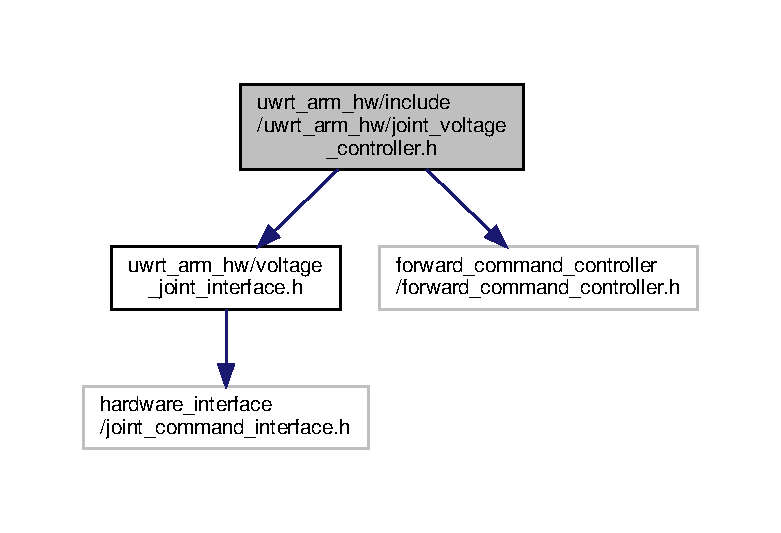
\includegraphics[width=350pt]{joint__voltage__controller_8h__incl}
\end{center}
\end{figure}
This graph shows which files directly or indirectly include this file\+:
\nopagebreak
\begin{figure}[H]
\begin{center}
\leavevmode
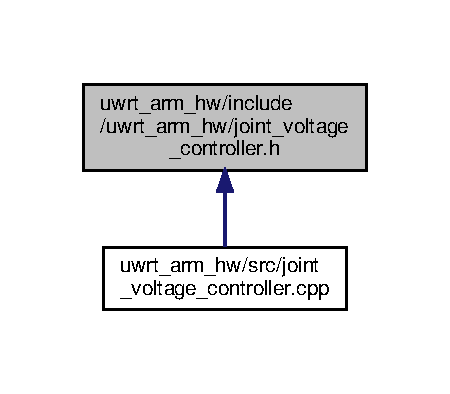
\includegraphics[width=216pt]{joint__voltage__controller_8h__dep__incl}
\end{center}
\end{figure}
\subsection*{Namespaces}
\begin{DoxyCompactItemize}
\item 
 \hyperlink{namespacevoltage__controllers}{voltage\+\_\+controllers}
\end{DoxyCompactItemize}
\subsection*{Typedefs}
\begin{DoxyCompactItemize}
\item 
typedef forward\+\_\+command\+\_\+controller\+::\+Forward\+Command\+Controller$<$ \hyperlink{classhardware__interface_1_1_voltage_joint_interface}{hardware\+\_\+interface\+::\+Voltage\+Joint\+Interface} $>$ \hyperlink{namespacevoltage__controllers_a342a187a35760323139ce1cad77898a6}{voltage\+\_\+controllers\+::\+Joint\+Voltage\+Controller}
\begin{DoxyCompactList}\small\item\em Joint Voltage Controller. \end{DoxyCompactList}\end{DoxyCompactItemize}

\hypertarget{real__arm__control_8h}{}\section{uwrt\+\_\+arm\+\_\+hw/include/uwrt\+\_\+arm\+\_\+hw/real\+\_\+arm\+\_\+control.h File Reference}
\label{real__arm__control_8h}\index{uwrt\+\_\+arm\+\_\+hw/include/uwrt\+\_\+arm\+\_\+hw/real\+\_\+arm\+\_\+control.\+h@{uwrt\+\_\+arm\+\_\+hw/include/uwrt\+\_\+arm\+\_\+hw/real\+\_\+arm\+\_\+control.\+h}}
{\ttfamily \#include \char`\"{}uwrt\+\_\+arm\+\_\+hw/arm\+\_\+control\+\_\+loop.\+h\char`\"{}}\newline
Include dependency graph for real\+\_\+arm\+\_\+control.\+h\+:
\nopagebreak
\begin{figure}[H]
\begin{center}
\leavevmode
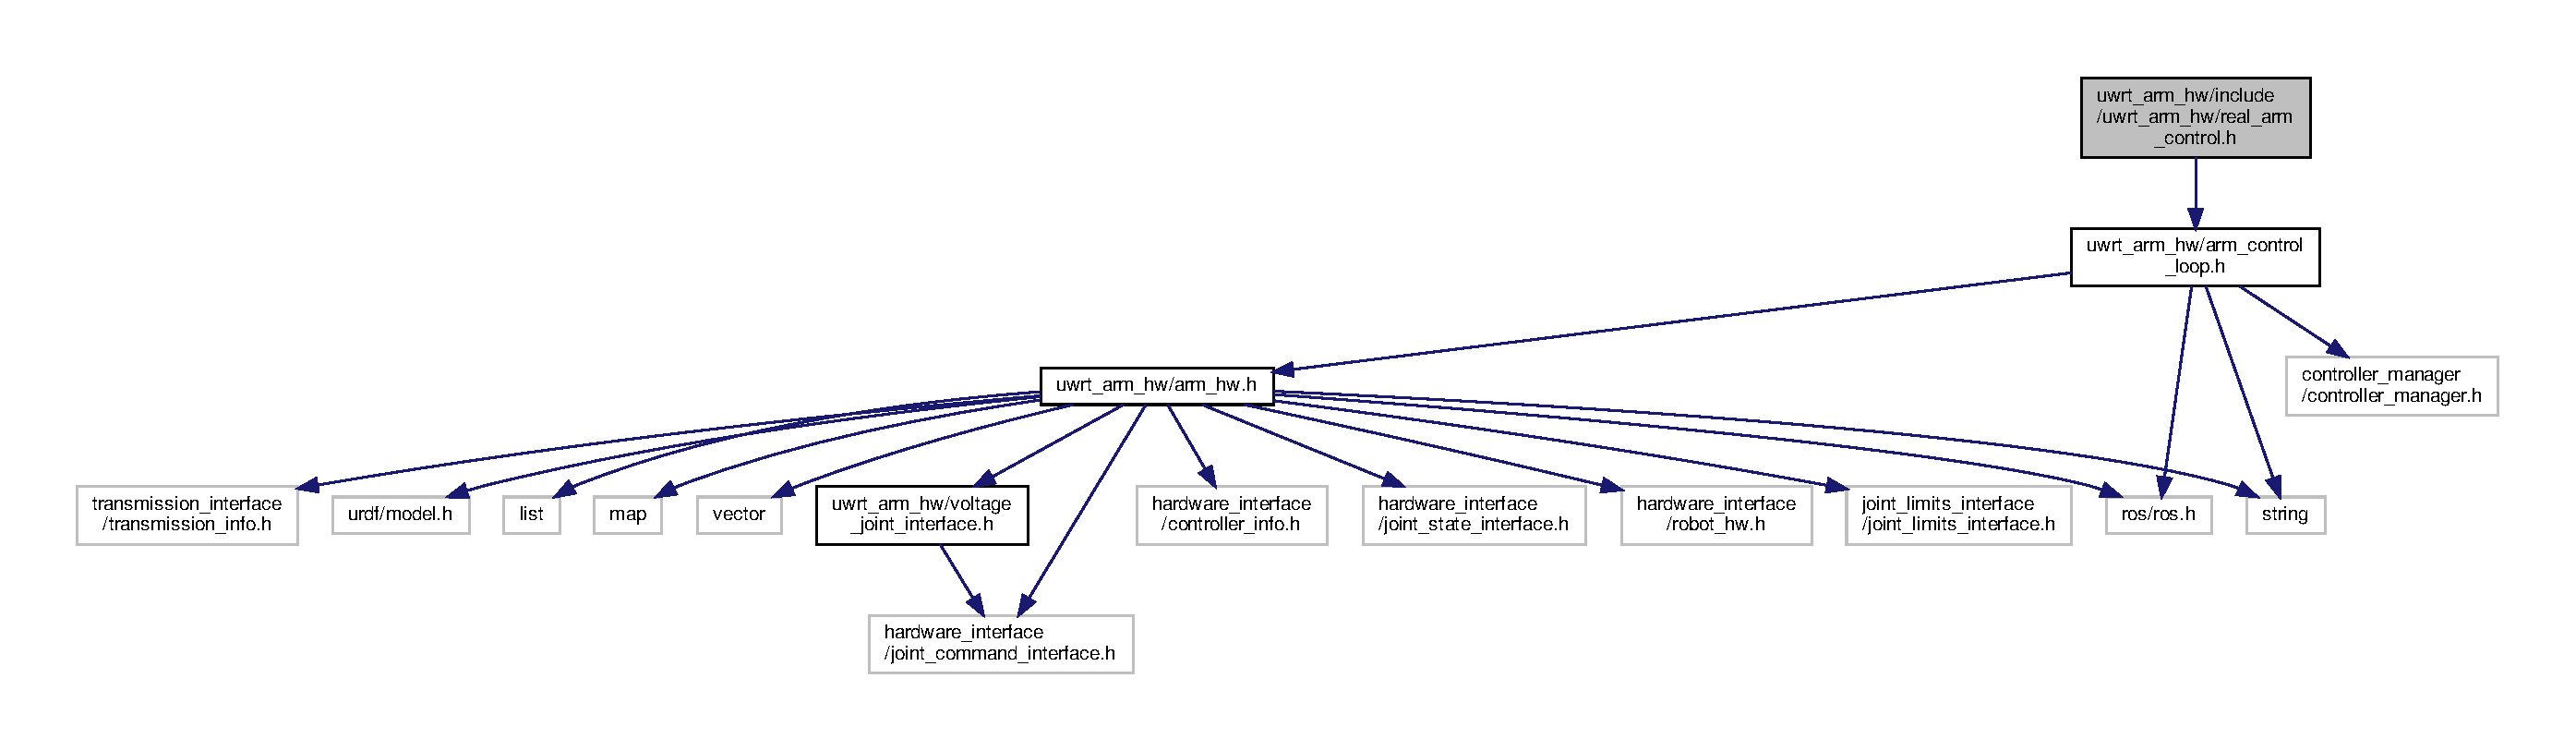
\includegraphics[width=350pt]{real__arm__control_8h__incl}
\end{center}
\end{figure}
This graph shows which files directly or indirectly include this file\+:
\nopagebreak
\begin{figure}[H]
\begin{center}
\leavevmode
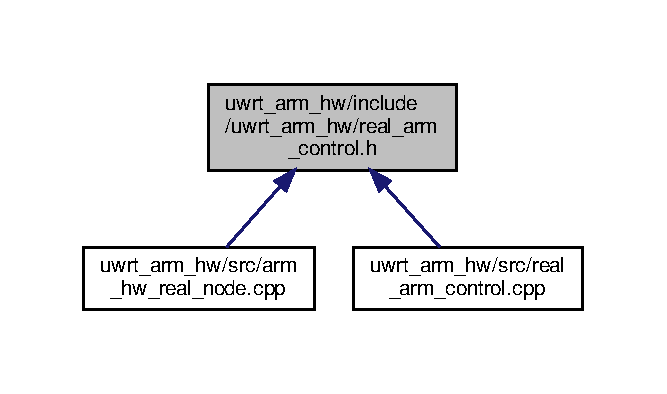
\includegraphics[width=320pt]{real__arm__control_8h__dep__incl}
\end{center}
\end{figure}
\subsection*{Classes}
\begin{DoxyCompactItemize}
\item 
class \hyperlink{classuwrt_1_1arm_1_1_real_arm_control}{uwrt\+::arm\+::\+Real\+Arm\+Control}
\end{DoxyCompactItemize}
\subsection*{Namespaces}
\begin{DoxyCompactItemize}
\item 
 \hyperlink{namespaceuwrt}{uwrt}
\item 
 \hyperlink{namespaceuwrt_1_1arm}{uwrt\+::arm}
\end{DoxyCompactItemize}

\hypertarget{voltage__joint__interface_8h}{}\section{uwrt\+\_\+arm\+\_\+hw/include/uwrt\+\_\+arm\+\_\+hw/voltage\+\_\+joint\+\_\+interface.h File Reference}
\label{voltage__joint__interface_8h}\index{uwrt\+\_\+arm\+\_\+hw/include/uwrt\+\_\+arm\+\_\+hw/voltage\+\_\+joint\+\_\+interface.\+h@{uwrt\+\_\+arm\+\_\+hw/include/uwrt\+\_\+arm\+\_\+hw/voltage\+\_\+joint\+\_\+interface.\+h}}
{\ttfamily \#include $<$hardware\+\_\+interface/joint\+\_\+command\+\_\+interface.\+h$>$}\newline
Include dependency graph for voltage\+\_\+joint\+\_\+interface.\+h\+:
\nopagebreak
\begin{figure}[H]
\begin{center}
\leavevmode
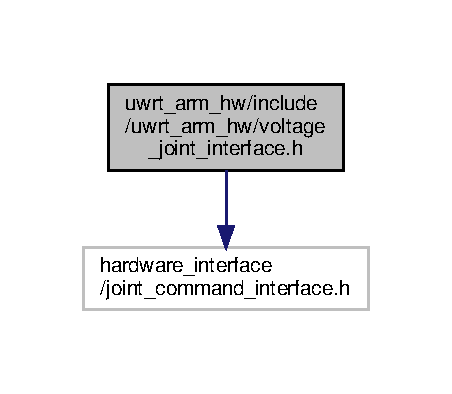
\includegraphics[width=217pt]{voltage__joint__interface_8h__incl}
\end{center}
\end{figure}
This graph shows which files directly or indirectly include this file\+:
\nopagebreak
\begin{figure}[H]
\begin{center}
\leavevmode
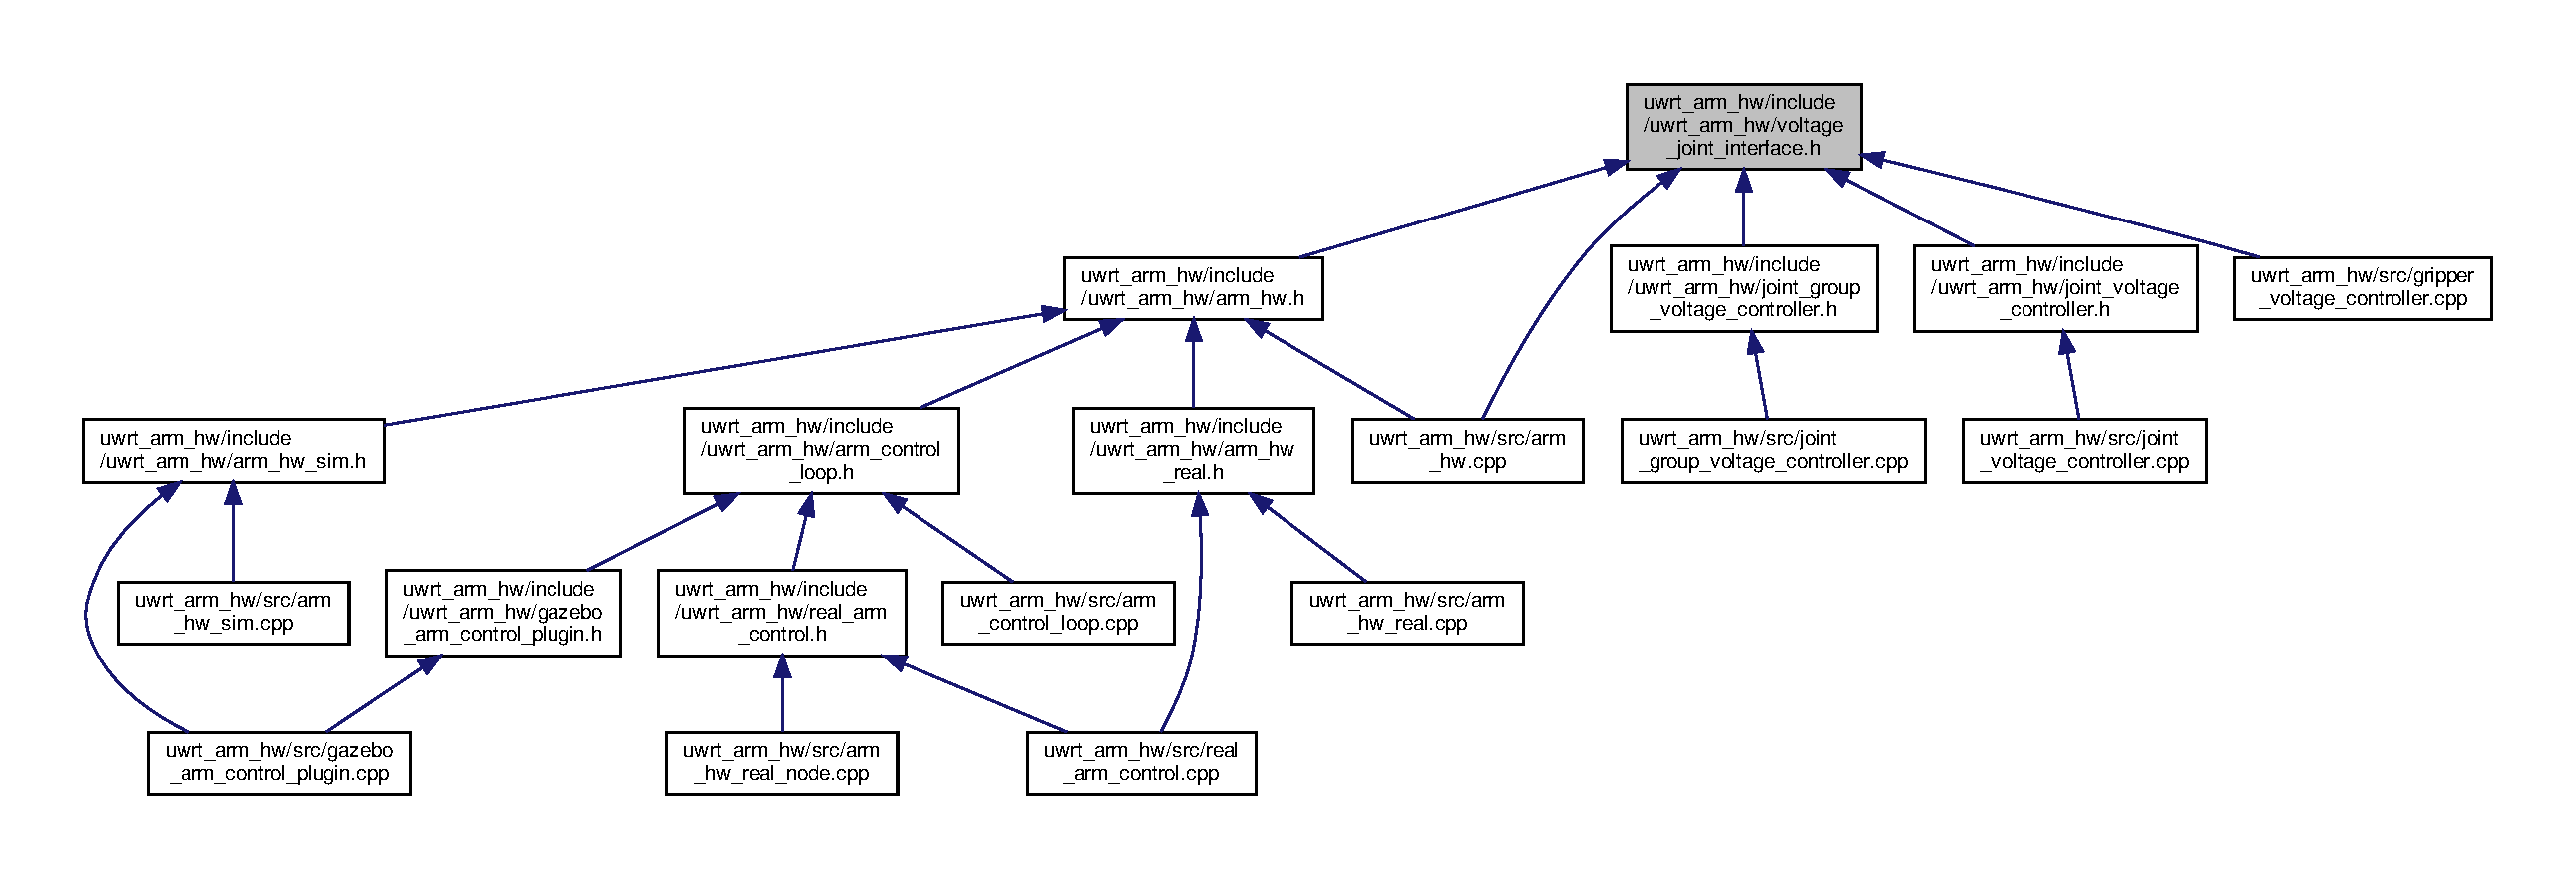
\includegraphics[width=350pt]{voltage__joint__interface_8h__dep__incl}
\end{center}
\end{figure}
\subsection*{Classes}
\begin{DoxyCompactItemize}
\item 
class \hyperlink{classhardware__interface_1_1_voltage_joint_interface}{hardware\+\_\+interface\+::\+Voltage\+Joint\+Interface}
\begin{DoxyCompactList}\small\item\em Joint\+Command\+Interface for commanding voltage-\/based joints. \end{DoxyCompactList}\end{DoxyCompactItemize}
\subsection*{Namespaces}
\begin{DoxyCompactItemize}
\item 
 \hyperlink{namespacehardware__interface}{hardware\+\_\+interface}
\end{DoxyCompactItemize}

\hypertarget{arm__control__loop_8cpp}{}\section{uwrt\+\_\+arm\+\_\+hw/src/arm\+\_\+control\+\_\+loop.cpp File Reference}
\label{arm__control__loop_8cpp}\index{uwrt\+\_\+arm\+\_\+hw/src/arm\+\_\+control\+\_\+loop.\+cpp@{uwrt\+\_\+arm\+\_\+hw/src/arm\+\_\+control\+\_\+loop.\+cpp}}
{\ttfamily \#include \char`\"{}uwrt\+\_\+arm\+\_\+hw/arm\+\_\+control\+\_\+loop.\+h\char`\"{}}\newline
{\ttfamily \#include $<$controller\+\_\+manager/controller\+\_\+manager.\+h$>$}\newline
{\ttfamily \#include $<$ros/ros.\+h$>$}\newline
{\ttfamily \#include $<$string$>$}\newline
Include dependency graph for arm\+\_\+control\+\_\+loop.\+cpp\+:
\nopagebreak
\begin{figure}[H]
\begin{center}
\leavevmode
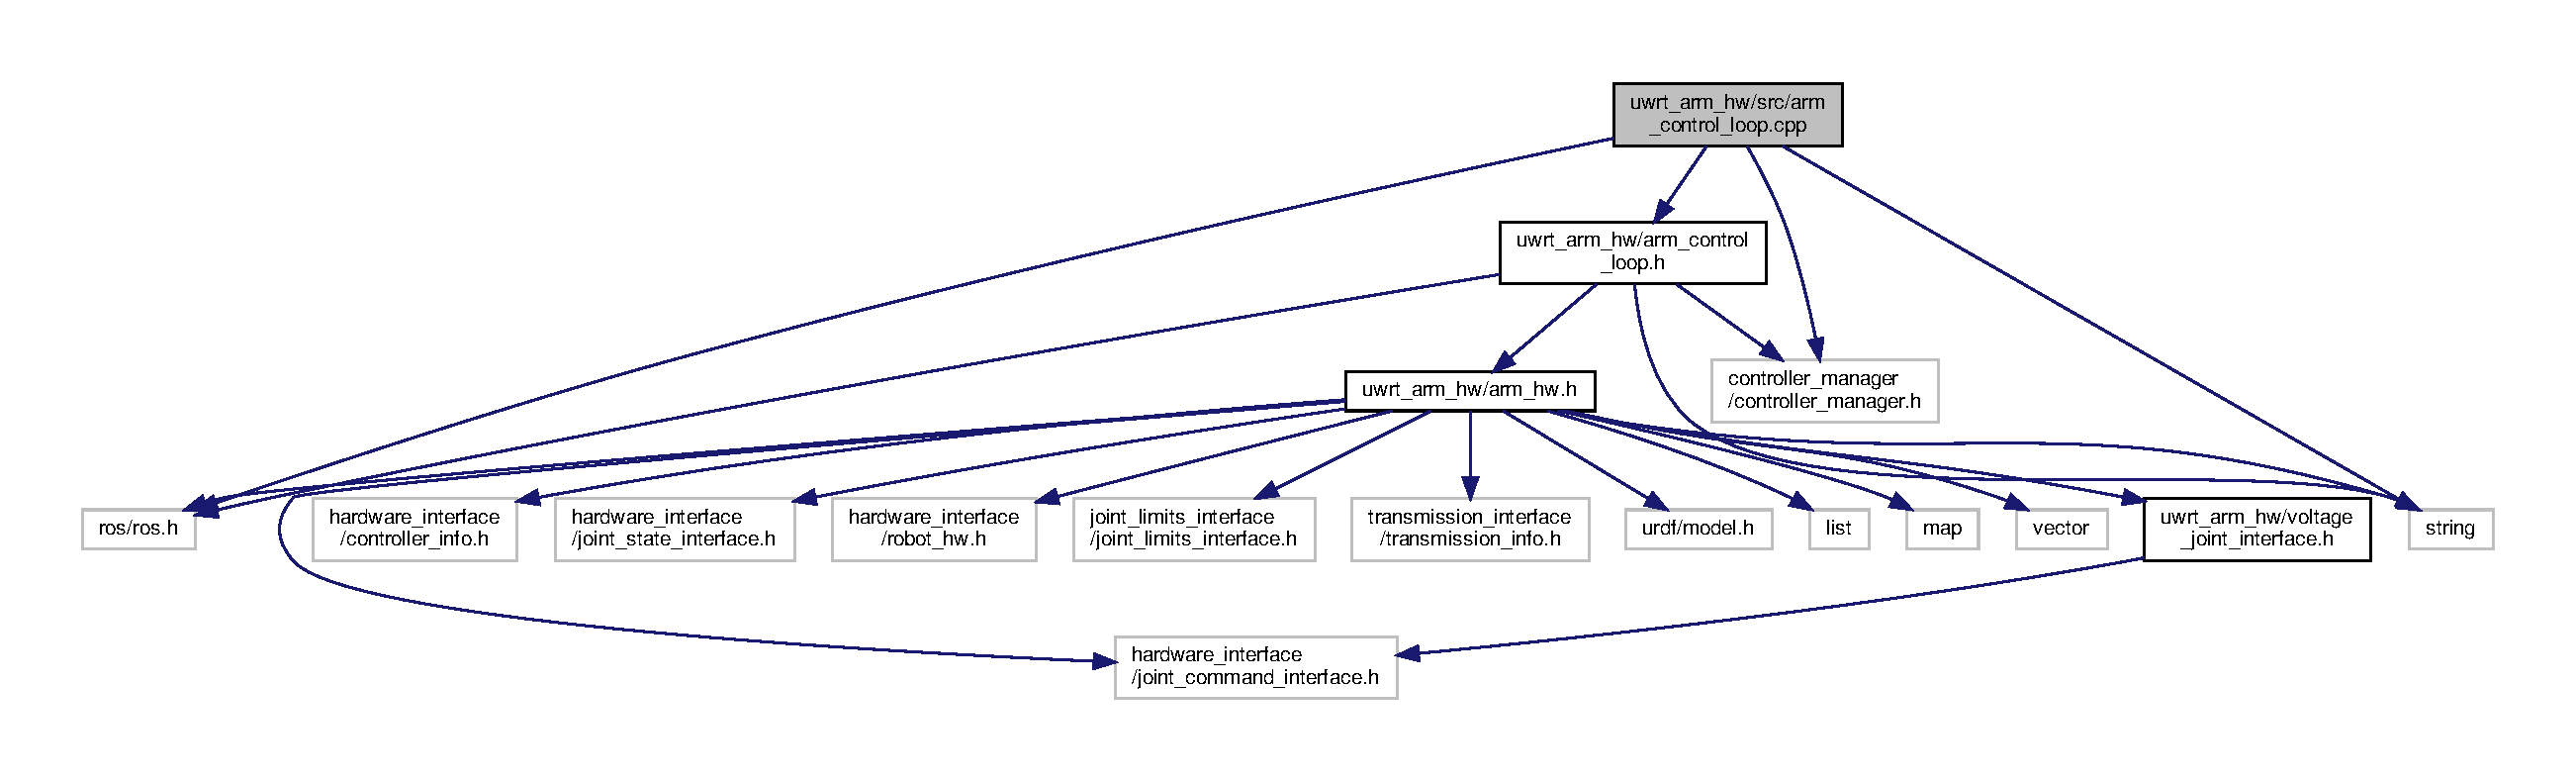
\includegraphics[width=350pt]{arm__control__loop_8cpp__incl}
\end{center}
\end{figure}
\subsection*{Namespaces}
\begin{DoxyCompactItemize}
\item 
 \hyperlink{namespaceuwrt}{uwrt}
\item 
 \hyperlink{namespaceuwrt_1_1arm}{uwrt\+::arm}
\end{DoxyCompactItemize}

\hypertarget{arm__hw_8cpp}{}\section{uwrt\+\_\+arm\+\_\+hw/src/arm\+\_\+hw.cpp File Reference}
\label{arm__hw_8cpp}\index{uwrt\+\_\+arm\+\_\+hw/src/arm\+\_\+hw.\+cpp@{uwrt\+\_\+arm\+\_\+hw/src/arm\+\_\+hw.\+cpp}}
{\ttfamily \#include \char`\"{}uwrt\+\_\+arm\+\_\+hw/arm\+\_\+hw.\+h\char`\"{}}\newline
{\ttfamily \#include \char`\"{}uwrt\+\_\+arm\+\_\+hw/voltage\+\_\+joint\+\_\+interface.\+h\char`\"{}}\newline
{\ttfamily \#include $<$joint\+\_\+limits\+\_\+interface/joint\+\_\+limits\+\_\+urdf.\+h$>$}\newline
{\ttfamily \#include $<$ros/ros.\+h$>$}\newline
{\ttfamily \#include $<$urdf\+\_\+model/joint.\+h$>$}\newline
{\ttfamily \#include $<$limits$>$}\newline
{\ttfamily \#include $<$list$>$}\newline
{\ttfamily \#include $<$string$>$}\newline
Include dependency graph for arm\+\_\+hw.\+cpp\+:
\nopagebreak
\begin{figure}[H]
\begin{center}
\leavevmode
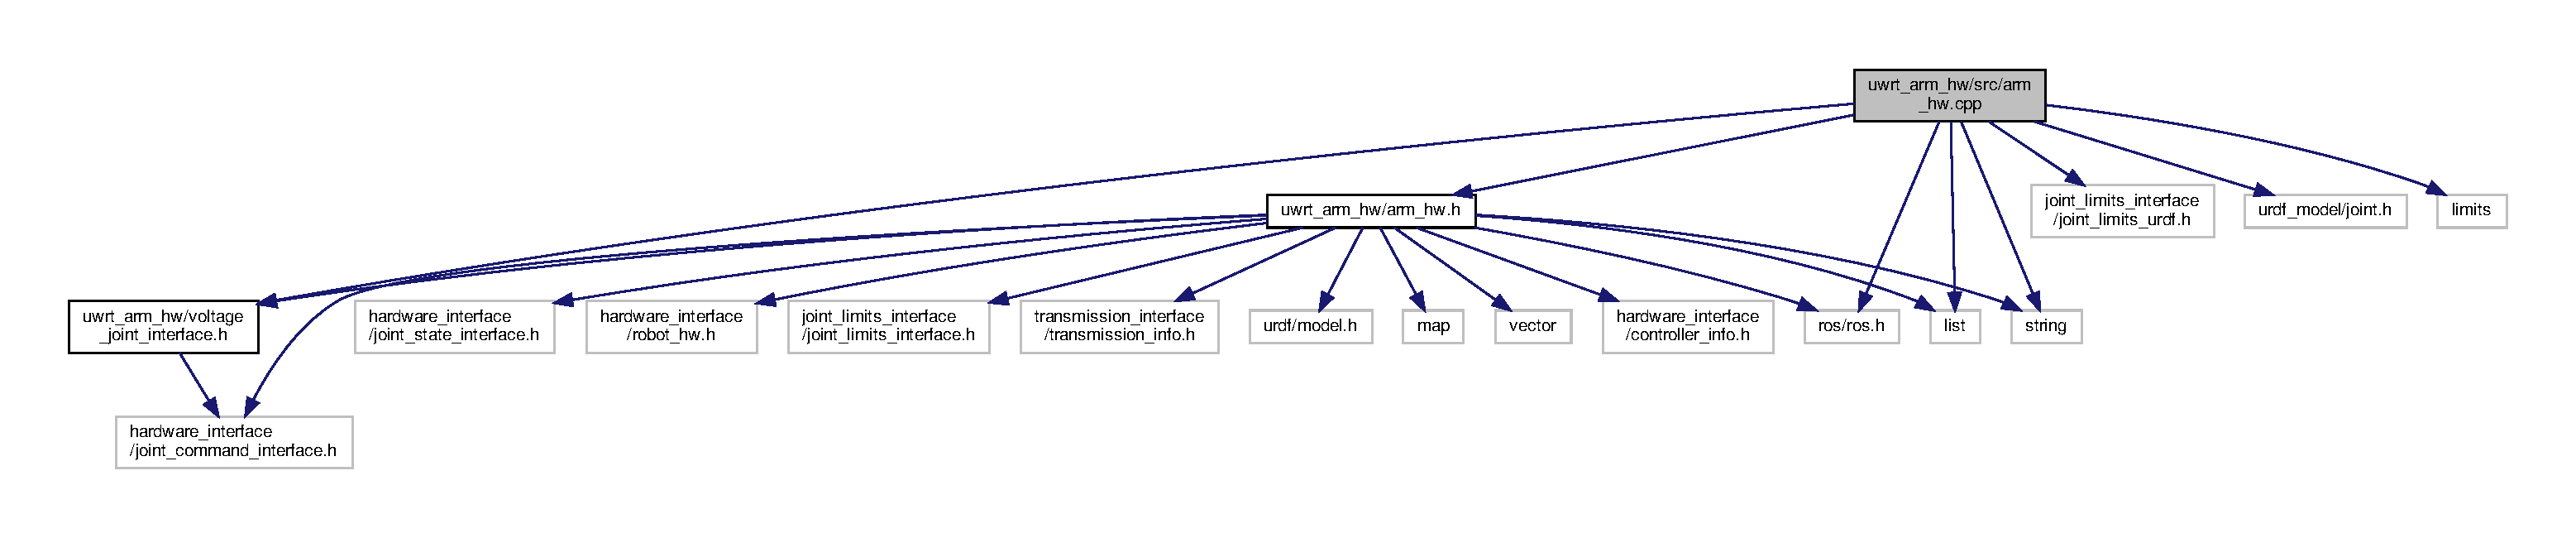
\includegraphics[width=350pt]{arm__hw_8cpp__incl}
\end{center}
\end{figure}
\subsection*{Namespaces}
\begin{DoxyCompactItemize}
\item 
 \hyperlink{namespaceuwrt}{uwrt}
\item 
 \hyperlink{namespaceuwrt_1_1arm}{uwrt\+::arm}
\end{DoxyCompactItemize}

\hypertarget{arm__hw__real_8cpp}{}\section{uwrt\+\_\+arm\+\_\+hw/src/arm\+\_\+hw\+\_\+real.cpp File Reference}
\label{arm__hw__real_8cpp}\index{uwrt\+\_\+arm\+\_\+hw/src/arm\+\_\+hw\+\_\+real.\+cpp@{uwrt\+\_\+arm\+\_\+hw/src/arm\+\_\+hw\+\_\+real.\+cpp}}
{\ttfamily \#include \char`\"{}uwrt\+\_\+arm\+\_\+hw/arm\+\_\+hw\+\_\+real.\+h\char`\"{}}\newline
{\ttfamily \#include \char`\"{}uwrt\+\_\+arm\+\_\+hw/can\+\_\+config.\+h\char`\"{}}\newline
{\ttfamily \#include $<$ros/ros.\+h$>$}\newline
{\ttfamily \#include $<$linux/can.\+h$>$}\newline
{\ttfamily \#include $<$linux/can/raw.\+h$>$}\newline
{\ttfamily \#include $<$string$>$}\newline
{\ttfamily \#include $<$sys/ioctl.\+h$>$}\newline
{\ttfamily \#include $<$sys/socket.\+h$>$}\newline
Include dependency graph for arm\+\_\+hw\+\_\+real.\+cpp\+:
\nopagebreak
\begin{figure}[H]
\begin{center}
\leavevmode
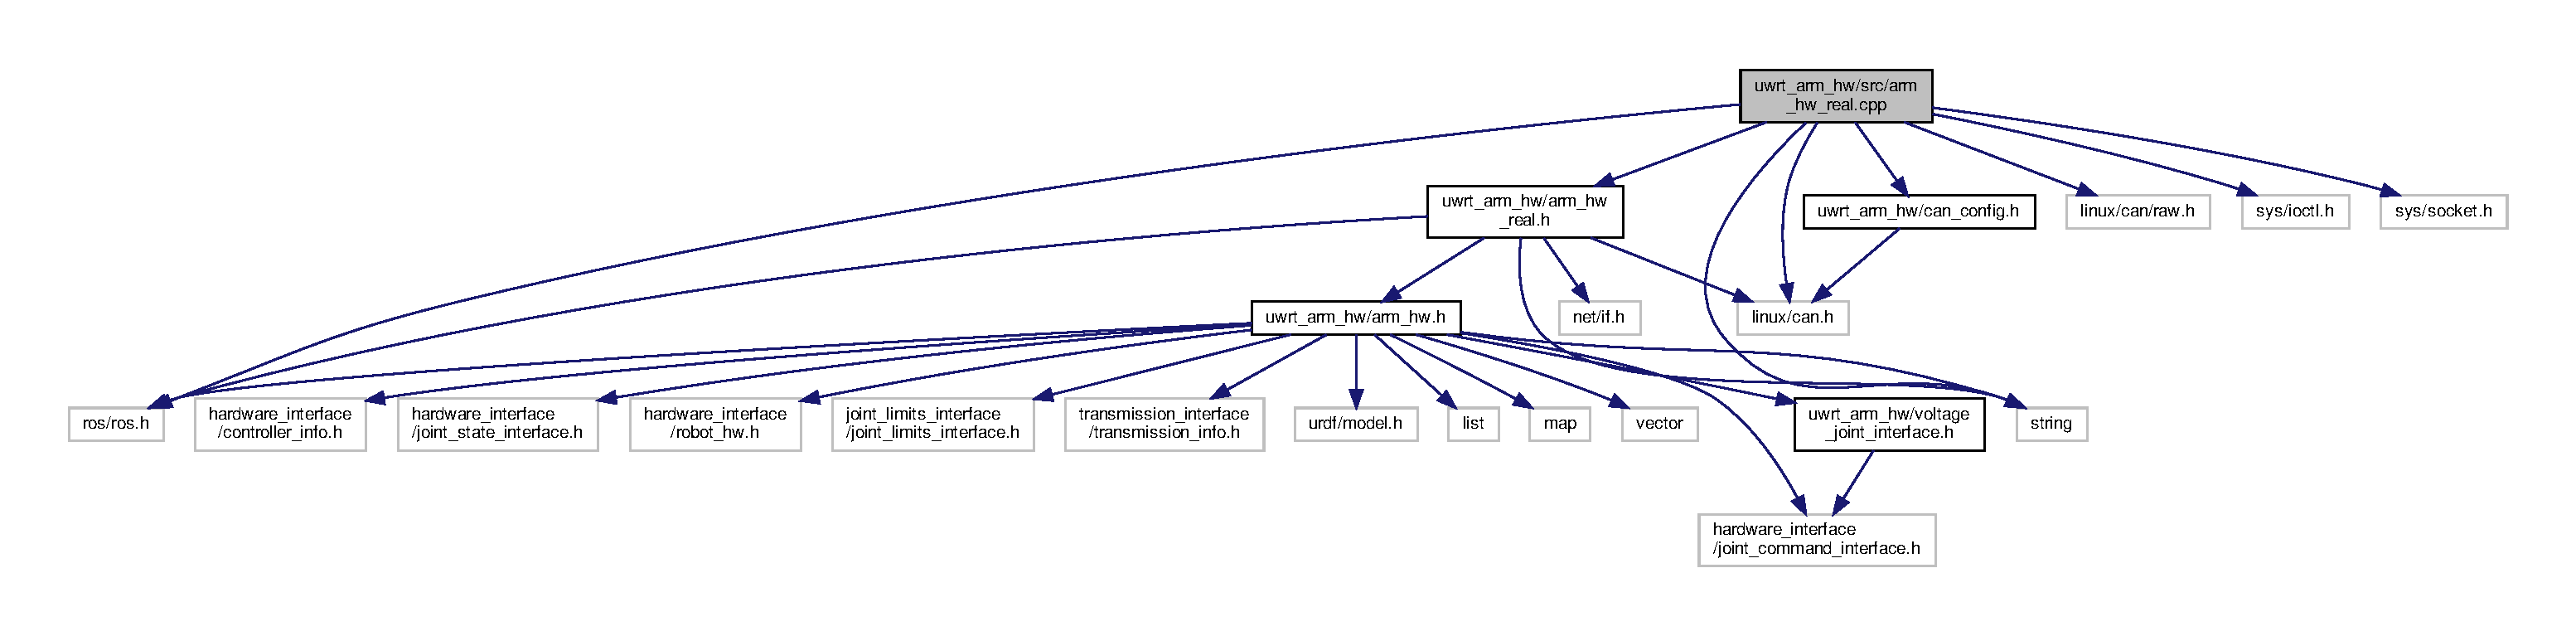
\includegraphics[width=350pt]{arm__hw__real_8cpp__incl}
\end{center}
\end{figure}
\subsection*{Namespaces}
\begin{DoxyCompactItemize}
\item 
 \hyperlink{namespaceuwrt}{uwrt}
\item 
 \hyperlink{namespaceuwrt_1_1arm}{uwrt\+::arm}
\end{DoxyCompactItemize}

\hypertarget{arm__hw__real__node_8cpp}{}\section{uwrt\+\_\+arm\+\_\+hw/src/arm\+\_\+hw\+\_\+real\+\_\+node.cpp File Reference}
\label{arm__hw__real__node_8cpp}\index{uwrt\+\_\+arm\+\_\+hw/src/arm\+\_\+hw\+\_\+real\+\_\+node.\+cpp@{uwrt\+\_\+arm\+\_\+hw/src/arm\+\_\+hw\+\_\+real\+\_\+node.\+cpp}}
{\ttfamily \#include \char`\"{}uwrt\+\_\+arm\+\_\+hw/real\+\_\+arm\+\_\+control.\+h\char`\"{}}\newline
{\ttfamily \#include $<$ros/ros.\+h$>$}\newline
Include dependency graph for arm\+\_\+hw\+\_\+real\+\_\+node.\+cpp\+:
\nopagebreak
\begin{figure}[H]
\begin{center}
\leavevmode
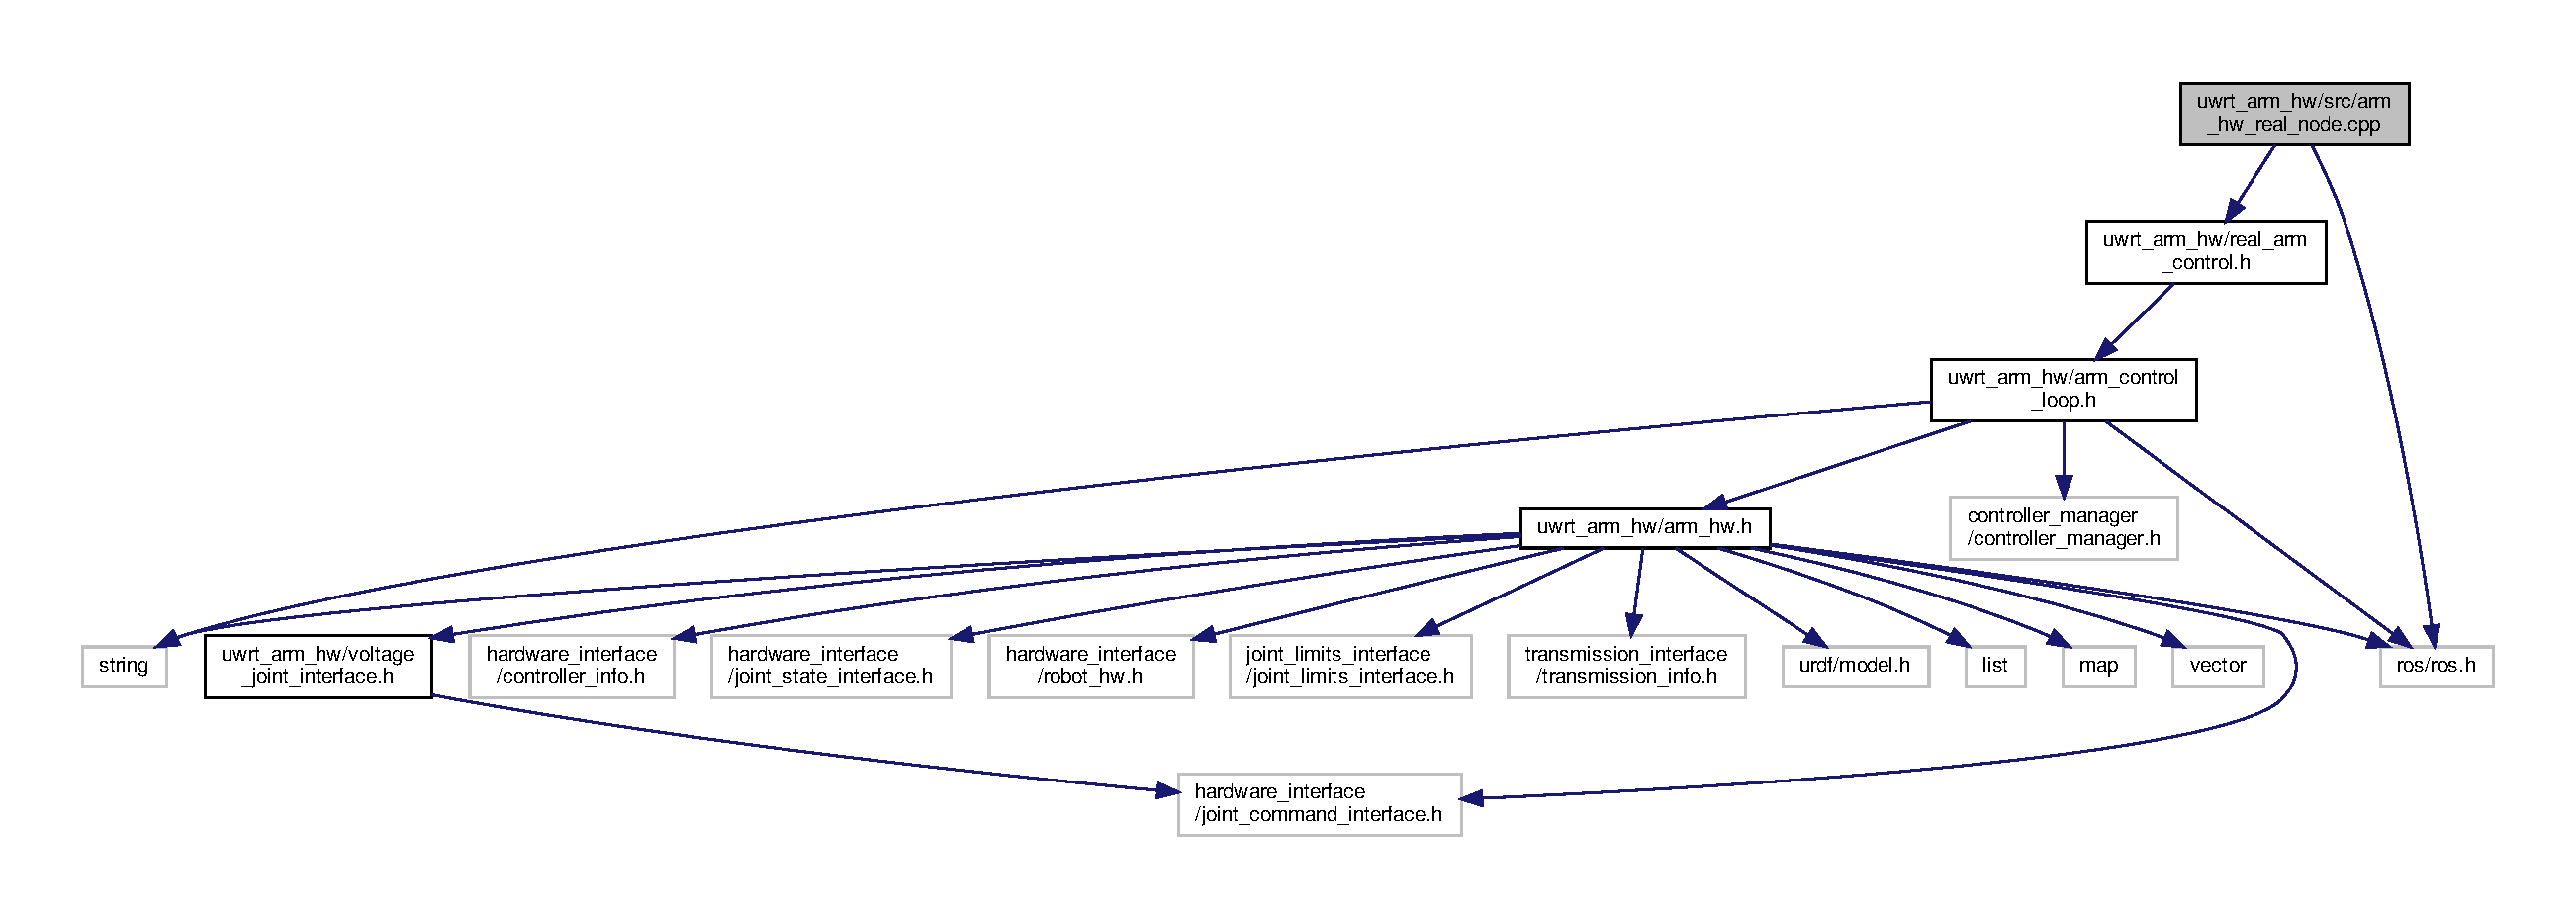
\includegraphics[width=350pt]{arm__hw__real__node_8cpp__incl}
\end{center}
\end{figure}
\subsection*{Functions}
\begin{DoxyCompactItemize}
\item 
int \hyperlink{arm__hw__real__node_8cpp_a3c04138a5bfe5d72780bb7e82a18e627}{main} (int argc, char $\ast$$\ast$argv)
\end{DoxyCompactItemize}


\subsection{Function Documentation}
\mbox{\Hypertarget{arm__hw__real__node_8cpp_a3c04138a5bfe5d72780bb7e82a18e627}\label{arm__hw__real__node_8cpp_a3c04138a5bfe5d72780bb7e82a18e627}} 
\index{arm\+\_\+hw\+\_\+real\+\_\+node.\+cpp@{arm\+\_\+hw\+\_\+real\+\_\+node.\+cpp}!main@{main}}
\index{main@{main}!arm\+\_\+hw\+\_\+real\+\_\+node.\+cpp@{arm\+\_\+hw\+\_\+real\+\_\+node.\+cpp}}
\subsubsection{\texorpdfstring{main()}{main()}}
{\footnotesize\ttfamily int main (\begin{DoxyParamCaption}\item[{int}]{argc,  }\item[{char $\ast$$\ast$}]{argv }\end{DoxyParamCaption})}

Copyright (c) 2020 Somesh Daga \href{mailto:s2daga@uwaterloo.ca}{\tt s2daga@uwaterloo.\+ca}

Permission is hereby granted, free of charge, to any person obtaining a copy of this software and associated documentation files (the \char`\"{}\+Software\char`\"{}), to deal in the Software without restriction, including without limitation the rights to use, copy, modify, merge, publish, distribute, sublicense, and/or sell copies of the Software, and to permit persons to whom the Software is furnished to do so, subject to the following conditions\+:

The above copyright notice and this permission notice shall be included in all copies or substantial portions of the Software.

T\+HE S\+O\+F\+T\+W\+A\+RE IS P\+R\+O\+V\+I\+D\+ED \char`\"{}\+A\+S I\+S\char`\"{}, W\+I\+T\+H\+O\+UT W\+A\+R\+R\+A\+N\+TY OF A\+NY K\+I\+ND, E\+X\+P\+R\+E\+SS OR I\+M\+P\+L\+I\+ED, I\+N\+C\+L\+U\+D\+I\+NG B\+UT N\+OT L\+I\+M\+I\+T\+ED TO T\+HE W\+A\+R\+R\+A\+N\+T\+I\+ES OF M\+E\+R\+C\+H\+A\+N\+T\+A\+B\+I\+L\+I\+TY, F\+I\+T\+N\+E\+SS F\+OR A P\+A\+R\+T\+I\+C\+U\+L\+AR P\+U\+R\+P\+O\+SE A\+ND N\+O\+N\+I\+N\+F\+R\+I\+N\+G\+E\+M\+E\+NT. IN NO E\+V\+E\+NT S\+H\+A\+LL T\+HE A\+U\+T\+H\+O\+RS OR C\+O\+P\+Y\+R\+I\+G\+HT H\+O\+L\+D\+E\+RS BE L\+I\+A\+B\+LE F\+OR A\+NY C\+L\+A\+IM, D\+A\+M\+A\+G\+ES OR O\+T\+H\+ER L\+I\+A\+B\+I\+L\+I\+TY, W\+H\+E\+T\+H\+ER IN AN A\+C\+T\+I\+ON OF C\+O\+N\+T\+R\+A\+CT, T\+O\+RT OR O\+T\+H\+E\+R\+W\+I\+SE, A\+R\+I\+S\+I\+NG F\+R\+OM, O\+UT OF OR IN C\+O\+N\+N\+E\+C\+T\+I\+ON W\+I\+TH T\+HE S\+O\+F\+T\+W\+A\+RE OR T\+HE U\+SE OR O\+T\+H\+ER D\+E\+A\+L\+I\+N\+GS IN T\+HE S\+O\+F\+T\+W\+A\+RE. 
\hypertarget{arm__hw__sim_8cpp}{}\section{uwrt\+\_\+arm\+\_\+hw/src/arm\+\_\+hw\+\_\+sim.cpp File Reference}
\label{arm__hw__sim_8cpp}\index{uwrt\+\_\+arm\+\_\+hw/src/arm\+\_\+hw\+\_\+sim.\+cpp@{uwrt\+\_\+arm\+\_\+hw/src/arm\+\_\+hw\+\_\+sim.\+cpp}}
{\ttfamily \#include \char`\"{}uwrt\+\_\+arm\+\_\+hw/arm\+\_\+hw\+\_\+sim.\+h\char`\"{}}\newline
{\ttfamily \#include $<$angles/angles.\+h$>$}\newline
{\ttfamily \#include $<$ros/ros.\+h$>$}\newline
{\ttfamily \#include $<$string$>$}\newline
{\ttfamily \#include $<$vector$>$}\newline
Include dependency graph for arm\+\_\+hw\+\_\+sim.\+cpp\+:
\nopagebreak
\begin{figure}[H]
\begin{center}
\leavevmode
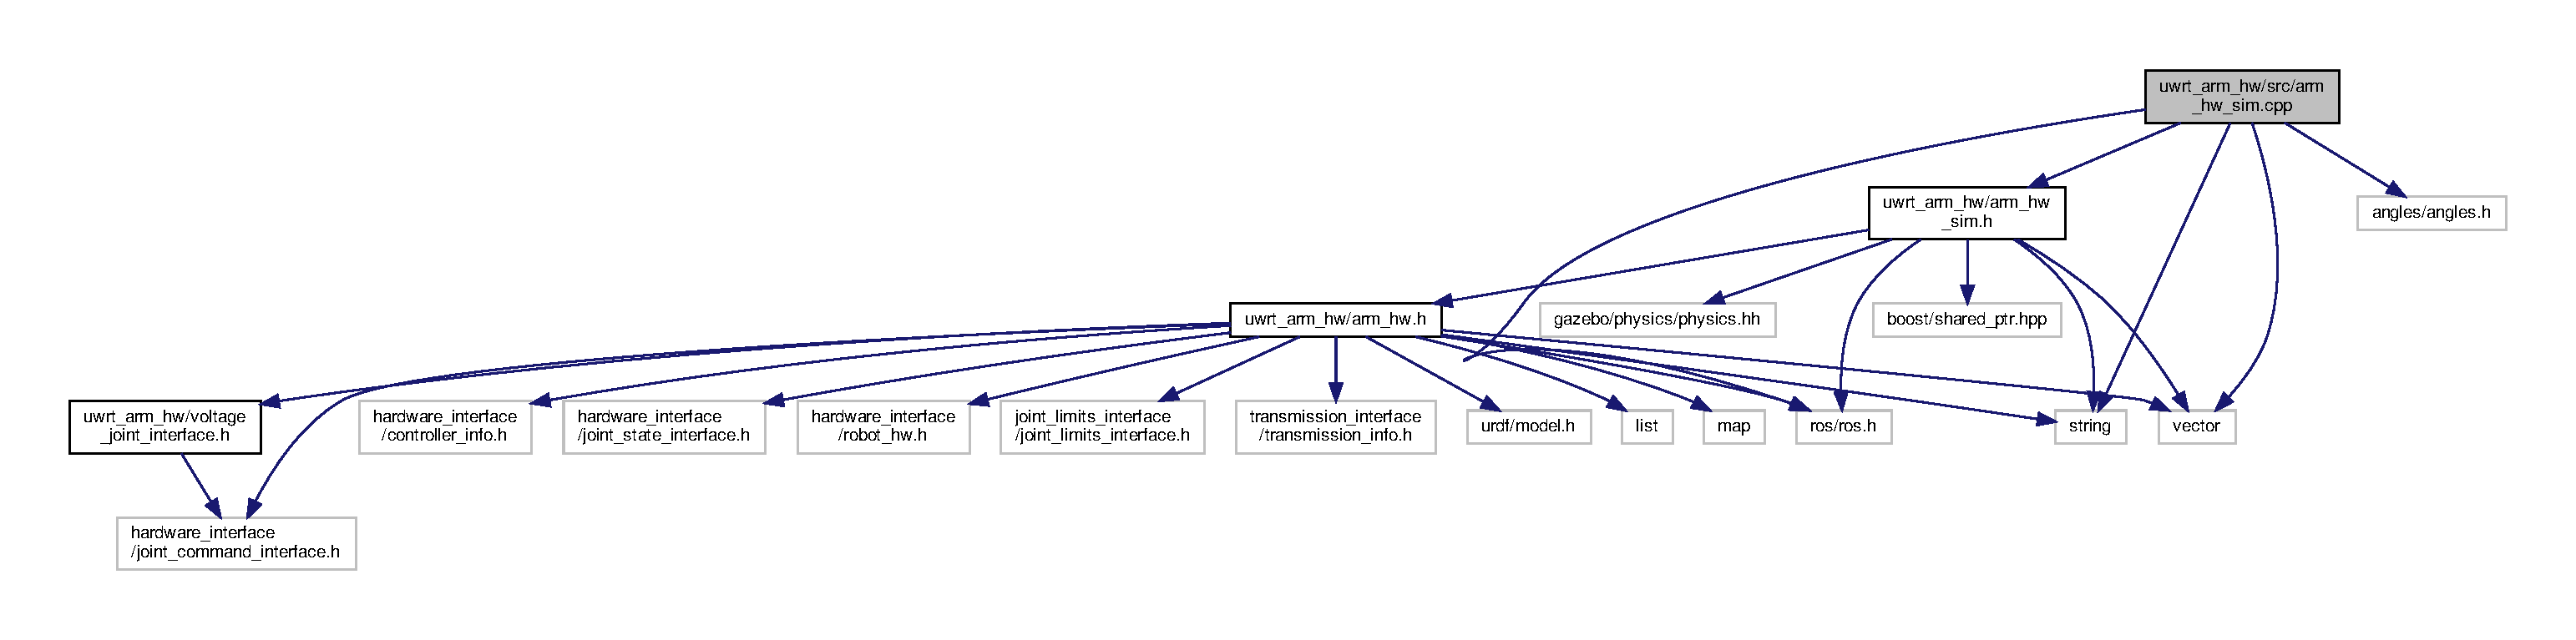
\includegraphics[width=350pt]{arm__hw__sim_8cpp__incl}
\end{center}
\end{figure}
\subsection*{Namespaces}
\begin{DoxyCompactItemize}
\item 
 \hyperlink{namespaceuwrt}{uwrt}
\item 
 \hyperlink{namespaceuwrt_1_1arm}{uwrt\+::arm}
\end{DoxyCompactItemize}

\hypertarget{gazebo__arm__control__plugin_8cpp}{}\section{uwrt\+\_\+arm\+\_\+hw/src/gazebo\+\_\+arm\+\_\+control\+\_\+plugin.cpp File Reference}
\label{gazebo__arm__control__plugin_8cpp}\index{uwrt\+\_\+arm\+\_\+hw/src/gazebo\+\_\+arm\+\_\+control\+\_\+plugin.\+cpp@{uwrt\+\_\+arm\+\_\+hw/src/gazebo\+\_\+arm\+\_\+control\+\_\+plugin.\+cpp}}
{\ttfamily \#include \char`\"{}uwrt\+\_\+arm\+\_\+hw/gazebo\+\_\+arm\+\_\+control\+\_\+plugin.\+h\char`\"{}}\newline
{\ttfamily \#include \char`\"{}uwrt\+\_\+arm\+\_\+hw/arm\+\_\+hw\+\_\+sim.\+h\char`\"{}}\newline
{\ttfamily \#include $<$ros/ros.\+h$>$}\newline
{\ttfamily \#include $<$string$>$}\newline
Include dependency graph for gazebo\+\_\+arm\+\_\+control\+\_\+plugin.\+cpp\+:
\nopagebreak
\begin{figure}[H]
\begin{center}
\leavevmode
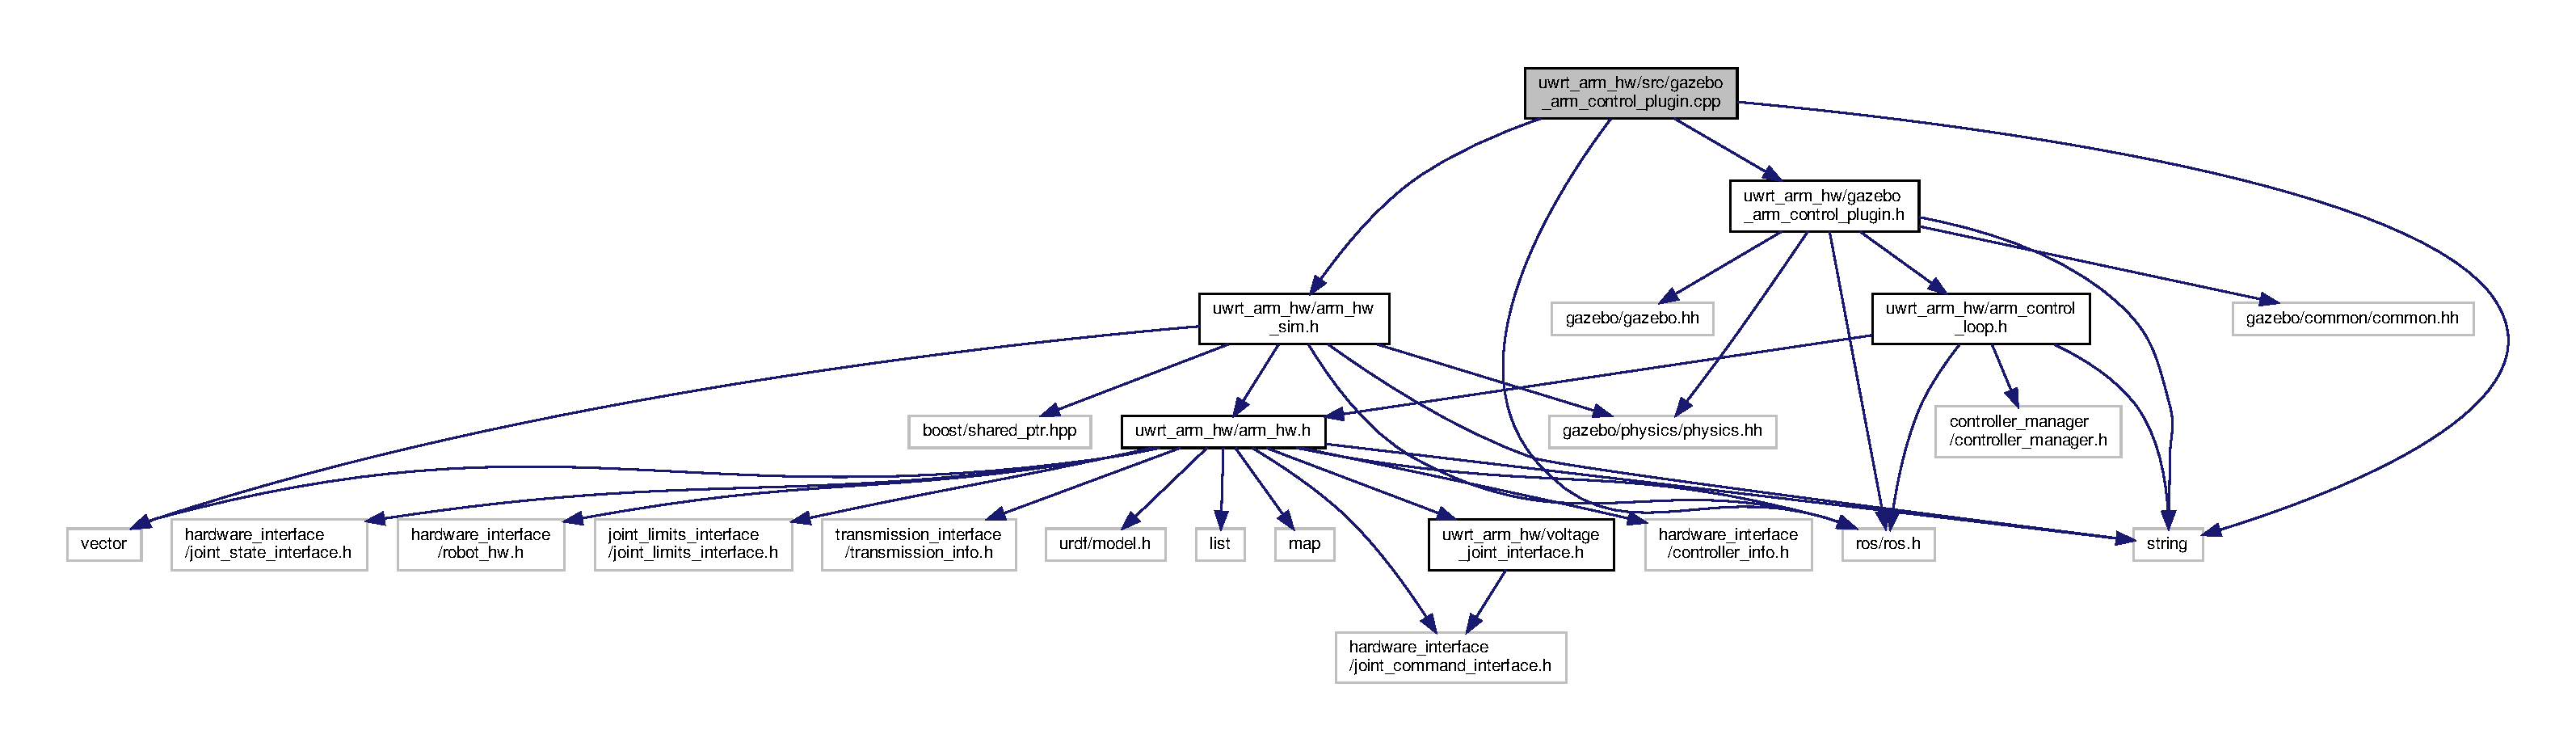
\includegraphics[width=350pt]{gazebo__arm__control__plugin_8cpp__incl}
\end{center}
\end{figure}
\subsection*{Namespaces}
\begin{DoxyCompactItemize}
\item 
 \hyperlink{namespaceuwrt}{uwrt}
\item 
 \hyperlink{namespaceuwrt_1_1arm}{uwrt\+::arm}
\end{DoxyCompactItemize}
\subsection*{Functions}
\begin{DoxyCompactItemize}
\item 
\hyperlink{namespaceuwrt_1_1arm_a1cd9b55d4936d61e403fc111a9f444c2}{uwrt\+::arm\+::\+G\+Z\+\_\+\+R\+E\+G\+I\+S\+T\+E\+R\+\_\+\+M\+O\+D\+E\+L\+\_\+\+P\+L\+U\+G\+IN} (Gazebo\+Arm\+Control\+Plugin)
\end{DoxyCompactItemize}

\hypertarget{gripper__voltage__controller_8cpp}{}\section{uwrt\+\_\+arm\+\_\+hw/src/gripper\+\_\+voltage\+\_\+controller.cpp File Reference}
\label{gripper__voltage__controller_8cpp}\index{uwrt\+\_\+arm\+\_\+hw/src/gripper\+\_\+voltage\+\_\+controller.\+cpp@{uwrt\+\_\+arm\+\_\+hw/src/gripper\+\_\+voltage\+\_\+controller.\+cpp}}
{\ttfamily \#include \char`\"{}uwrt\+\_\+arm\+\_\+hw/voltage\+\_\+joint\+\_\+interface.\+h\char`\"{}}\newline
{\ttfamily \#include $<$pluginlib/class\+\_\+list\+\_\+macros.\+hpp$>$}\newline
{\ttfamily \#include $<$gripper\+\_\+action\+\_\+controller/gripper\+\_\+action\+\_\+controller.\+h$>$}\newline
Include dependency graph for gripper\+\_\+voltage\+\_\+controller.\+cpp\+:
\nopagebreak
\begin{figure}[H]
\begin{center}
\leavevmode
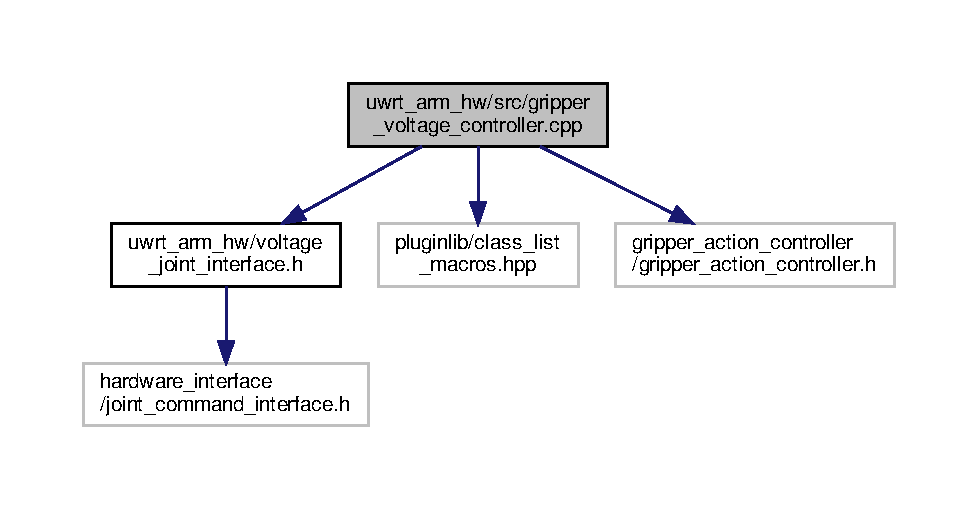
\includegraphics[width=350pt]{gripper__voltage__controller_8cpp__incl}
\end{center}
\end{figure}
\subsection*{Namespaces}
\begin{DoxyCompactItemize}
\item 
 \hyperlink{namespacevoltage__controllers}{voltage\+\_\+controllers}
\end{DoxyCompactItemize}
\subsection*{Typedefs}
\begin{DoxyCompactItemize}
\item 
typedef gripper\+\_\+action\+\_\+controller\+::\+Gripper\+Action\+Controller$<$ \hyperlink{classhardware__interface_1_1_voltage_joint_interface}{hardware\+\_\+interface\+::\+Voltage\+Joint\+Interface} $>$ \hyperlink{namespacevoltage__controllers_a56f9a4de5492f0b87d819d8db50835fd}{voltage\+\_\+controllers\+::\+Gripper\+Action\+Controller}
\begin{DoxyCompactList}\small\item\em Gripper action controller that sends commands to a {\bfseries voltage} interface. \end{DoxyCompactList}\end{DoxyCompactItemize}

\hypertarget{joint__group__voltage__controller_8cpp}{}\section{uwrt\+\_\+arm\+\_\+hw/src/joint\+\_\+group\+\_\+voltage\+\_\+controller.cpp File Reference}
\label{joint__group__voltage__controller_8cpp}\index{uwrt\+\_\+arm\+\_\+hw/src/joint\+\_\+group\+\_\+voltage\+\_\+controller.\+cpp@{uwrt\+\_\+arm\+\_\+hw/src/joint\+\_\+group\+\_\+voltage\+\_\+controller.\+cpp}}
{\ttfamily \#include \char`\"{}uwrt\+\_\+arm\+\_\+hw/joint\+\_\+group\+\_\+voltage\+\_\+controller.\+h\char`\"{}}\newline
{\ttfamily \#include $<$pluginlib/class\+\_\+list\+\_\+macros.\+hpp$>$}\newline
Include dependency graph for joint\+\_\+group\+\_\+voltage\+\_\+controller.\+cpp\+:
\nopagebreak
\begin{figure}[H]
\begin{center}
\leavevmode
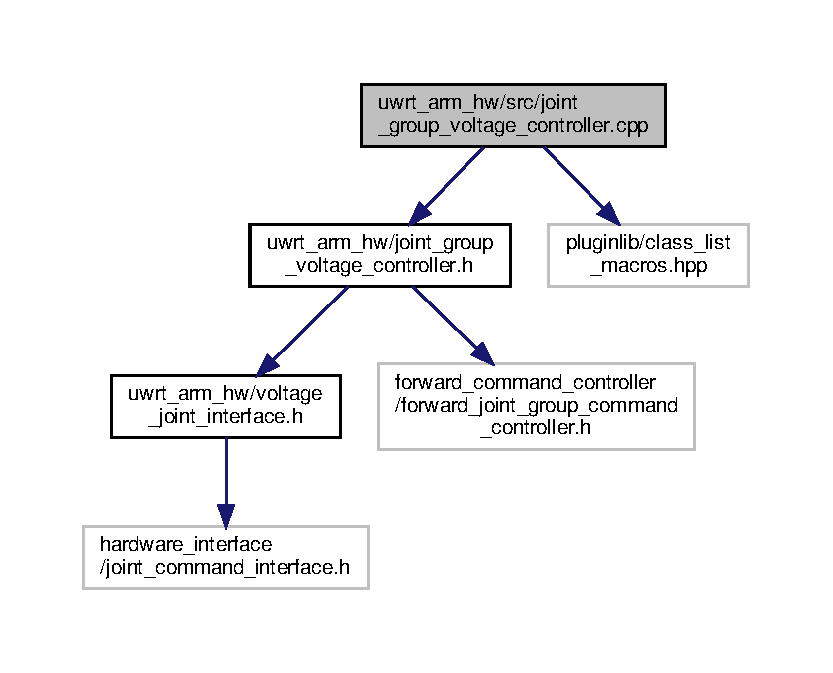
\includegraphics[width=350pt]{joint__group__voltage__controller_8cpp__incl}
\end{center}
\end{figure}

\hypertarget{joint__voltage__controller_8cpp}{}\section{uwrt\+\_\+arm\+\_\+hw/src/joint\+\_\+voltage\+\_\+controller.cpp File Reference}
\label{joint__voltage__controller_8cpp}\index{uwrt\+\_\+arm\+\_\+hw/src/joint\+\_\+voltage\+\_\+controller.\+cpp@{uwrt\+\_\+arm\+\_\+hw/src/joint\+\_\+voltage\+\_\+controller.\+cpp}}
{\ttfamily \#include \char`\"{}uwrt\+\_\+arm\+\_\+hw/joint\+\_\+voltage\+\_\+controller.\+h\char`\"{}}\newline
{\ttfamily \#include $<$pluginlib/class\+\_\+list\+\_\+macros.\+hpp$>$}\newline
Include dependency graph for joint\+\_\+voltage\+\_\+controller.\+cpp\+:
\nopagebreak
\begin{figure}[H]
\begin{center}
\leavevmode
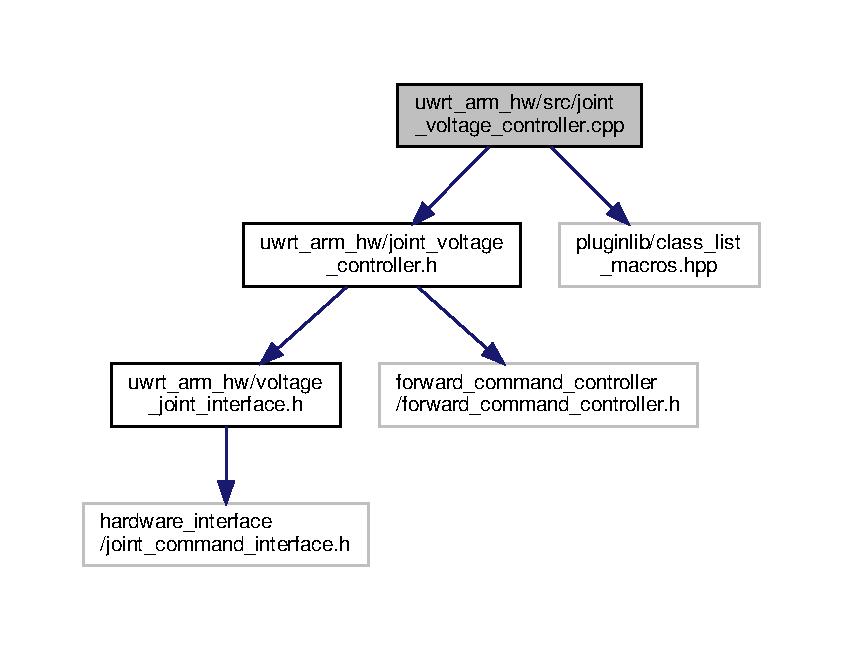
\includegraphics[width=350pt]{joint__voltage__controller_8cpp__incl}
\end{center}
\end{figure}

\hypertarget{real__arm__control_8cpp}{}\section{uwrt\+\_\+arm\+\_\+hw/src/real\+\_\+arm\+\_\+control.cpp File Reference}
\label{real__arm__control_8cpp}\index{uwrt\+\_\+arm\+\_\+hw/src/real\+\_\+arm\+\_\+control.\+cpp@{uwrt\+\_\+arm\+\_\+hw/src/real\+\_\+arm\+\_\+control.\+cpp}}
{\ttfamily \#include \char`\"{}uwrt\+\_\+arm\+\_\+hw/arm\+\_\+hw\+\_\+real.\+h\char`\"{}}\newline
{\ttfamily \#include \char`\"{}uwrt\+\_\+arm\+\_\+hw/real\+\_\+arm\+\_\+control.\+h\char`\"{}}\newline
{\ttfamily \#include $<$ros/ros.\+h$>$}\newline
{\ttfamily \#include $<$string$>$}\newline
Include dependency graph for real\+\_\+arm\+\_\+control.\+cpp\+:
\nopagebreak
\begin{figure}[H]
\begin{center}
\leavevmode
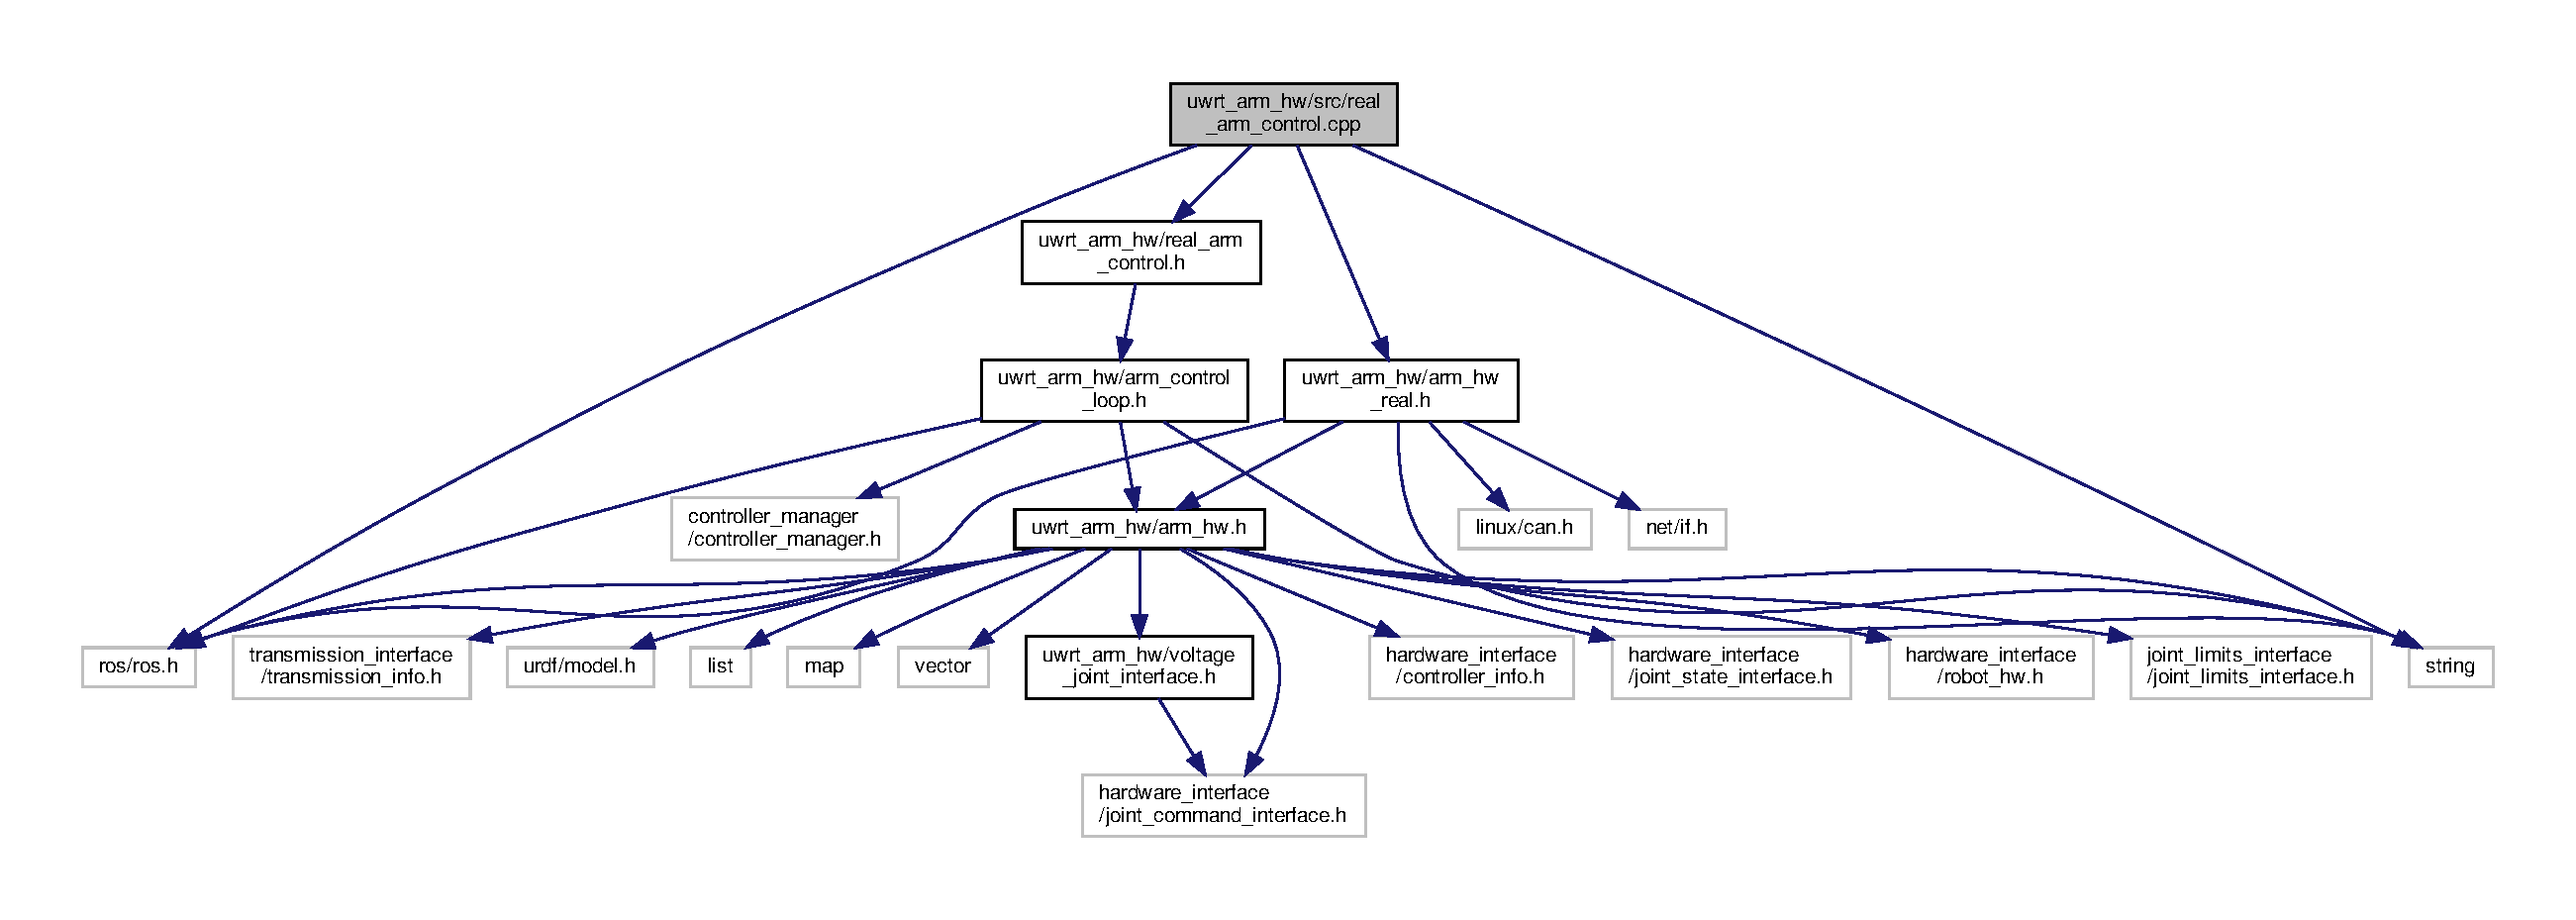
\includegraphics[width=350pt]{real__arm__control_8cpp__incl}
\end{center}
\end{figure}
\subsection*{Namespaces}
\begin{DoxyCompactItemize}
\item 
 \hyperlink{namespaceuwrt}{uwrt}
\item 
 \hyperlink{namespaceuwrt_1_1arm}{uwrt\+::arm}
\end{DoxyCompactItemize}

%--- End generated contents ---

% Index
\backmatter
\newpage
\phantomsection
\clearemptydoublepage
\addcontentsline{toc}{chapter}{Index}
\printindex

\end{document}
